
\tolerance 500   % suppresses moaning "`overfull \hbox"'.

\documentclass[11pt,english,a4paper,normalheadings,twoside,DIV9,BCOR10mm,listsleft,fleqn,leqno,abstracton,pointlessnumbers]{scrbook}

\usepackage[T1]{fontenc}
\usepackage[utf8]{inputenc}


%%%%%%%%%%%%%%%%%%%%%%%%%%%%%%%%%%%%%%%%%%%%%
%% These are the variables to configure the produced PDF file. Please
%% fill them out properly.
\def\university {Reutlingen University}						%% name the university here
\def\faculty {School of Informatics | Herman Hollerith Center}	%% and, also name the faculty
\def\titelname {Master-Thesis-Grodmeier}									%% name of the PDF document; in
													%% in the simple case, just use
													%% the thesis's title
\def\autorforinfo {Lukas Grodmeier}					%% name of the author of this document
\def\studentid{810112}				%% provide your Student Id
\def\email {lukas.grodmeier@student.reutlingen-university.de}			%% your e-mail address
\def\subjectname {TinyMLops}				%% please indicate, what the
									%% general area of your work is
\def\keywordsname {TinyMLops, TinyML, Life-Cycle-Management}	%% add a comma-separated list of
									%% of keywords to help document
									%% indexing

%%%%%%%%%%%%%%%%%%%%%%%%%%%%%%%%%%%%%%%%%%%%%
%% Specific variables for the Thesis:

% What is the thesis's type, BSc, MSc, etc.; don't forget the subject...
% For example, if you are going to write a Bachelor Thesis in DIB, just use the specification below.
% If you are doing a Masters Thesis, e.g., in DBE, just change the line below accordingly...
\def\doctype{Master Thesis in Digital Business Engineering (M.Sc.)}
%  What is the title of the thesis?
\def\title{On-Device MLOps: A Framework for Embedded Machine Learning in Resource-Constrained Systems}
%  Who are you?
\def\author{Lukas Grodmeier}
\def\studId{810112}
%  What is the hand-in date of the thesis?
\def\handindate{June 13, 2025}
%  Who is supervising you?
\def\firstSupervisor{Prof. Dr. Marco Kuhrmann}
\def\secondSupervisor{Prof. Dr. Christian Decker}

%% Selection of the AI utilization in this thesis: From the following three options, select this one
%% that applies. Use the comment function to enable the required option and to disable those
%% options that don't apply

% Option 1: No use of AI tools. 
%\def\AIToolsUse{I also confirm that I have not used any AI-based, content-generating tools.}

% Option 2: Mandatory labeling of AI tools with permitted use 
\def\AIToolsUse{I also confirm that the use of AI tools has been explicitly permitted by the examiner and that I have made use of them in my work. The AI tools used are attached to the thesis in accordance with the faculty's internal citation and documentation requirements. I only used content-generating AI tools for support and did not let the AI take over the core theses of my work. I am aware that the use of AI tools does not guarantee accuracy and that I am responsible for all AI-generated content in this thesis.}

% Option 3: Permission of content-generating AI tools without mandatory labeling 
%\def\AIToolsUse{I also confirm that I have only used content-generating AI tools in a supportive manner and have not allowed the AI to take over the core theses of my work. I am aware that the use of AI tools does not guarantee accuracy and that I am responsible for all AI-generated content in this thesis.}

%%%%%%%%%%%%%%%%%%%%%%%%%%%%%%%%%%%%%%%%%%%%%
%% definition of the document metric - DON'T CHANGE!!!
\usepackage[inner=2.5cm,outer=3cm,top=1cm,bottom=1cm,includeheadfoot]{geometry}
\usepackage{times}
\usepackage{amsmath}
\usepackage{amssymb}
\usepackage{amsthm}
\usepackage{amsbsy}
\usepackage{babel}
\usepackage{paralist}

\usepackage{xspace}

%%%%%%%%%%%%%%%%%%%%%%%%%%%%%%%%%%%%%%%%%%%%%
%% import of the packages for nice tables
\usepackage{array}
\usepackage{tabularx}
\usepackage{booktabs}
\usepackage{colortbl}
\usepackage{everysel}
\usepackage{framed}
\usepackage{ragged2e}

%%%%%%%%%%%%%%%%%%%%%%%%%%%%%%%%%%%%%%%%%%%%%
%% include the minitoc-package to generate fancy section TOC's
\usepackage{shorttoc}
\usepackage{minitoc}

%%%%%%%%%%%%%%%%%%%%%%%%%%%%%%%%%%%%%%%%%%%%%
%% definition of scaling table columns - requires the table packages
%% imported before
\newcolumntype{L}{>{\RaggedRight\arraybackslash}X}%
\newcolumntype{C}{>{\Centering\arraybackslash}X}%
\newcolumntype{R}{>{\RaggedLeft\arraybackslash}X}%

%% own
\newcolumntype{Y}{>{\RaggedRight\arraybackslash}X}


\newcommand{\opentableheader}{\toprule}
\newcommand{\closetableheader}{\toprule}

%%%%%%%%%%%%%%%%%%%%%%%%%%%%%%%%%%%%%%%%%%%%%
%% actual versions of the listings package:
%% ftp://ftp.dante.de/tex-archive/help/Catalogue/entries/listings.html
\usepackage{listings}
\usepackage{dotnet_new}

%% own packages
\usepackage[acronym]{glossaries} 
\newacronym{dsr}{DSR}{Design Science Research}
\newacronym{slr}{SLR}{Systematic Literature Review}
\newacronym{rq}{RQ}{Research Question}
\newacronym{sms}{SMS}{Systematic Mapping Study}
\newacronym{tinymlops}{TinyMLOps}{Tiny Machine Learning and Operations}
\newacronym{tinyml}{TinyML}{Tiny Machine Learning}
\newacronym{mlops}{MLOps}{Machine Learning and Operations}
\newacronym{lcm}{LCM}{Lifecycle Management}
\newacronym{ai}{AI}{Artificial Intelligence}
\newacronym{ci}{CI}{Continuous Integration}
\newacronym{cd}{CD}{Continuous Delivery}
\newacronym{ct}{CT}{Continuous Training}
\newacronym{ml}{ML}{Machine Learning}
\newacronym{devops}{DevOps}{Development and Operations}
\newacronym{mcu}{MCU}{Microcontroller Unit}
\newacronym{sbc}{SBC}{Single Board Computer}
\newacronym{iot}{IoT}{Internet of Things}
\newacronym{kb}{KB}{Kilobyte}
\newacronym{mb}{MB}{Megabyte}
\newacronym{gb}{GB}{Gigabyte}
\newacronym{mw}{mW}{Milliwatt}
\newacronym{rtos}{RTOS}{Real-Time Operating Systems}
\newacronym{tflm}{TFLM}{TensorFlow Lite Micro}
\newacronym{tfl}{TFL}{TensorFlow Lite}
\newacronym{tinylcm}{TinyLCM}{Tiny Machine Learning Lifecycle Management}
\newacronym{nas}{NAS}{Neural Architecture Search}
\newacronym{svm}{SVM}{Support Vector Machine}
\newacronym{knn}{KNN}{K-Nearest Neighbors}
\newacronym{pca}{PCA}{Pricipal Component Analysis}
\newacronym{cpu}{CPU}{Central Processing Unit}

\newacronym{ci_cd}{CI/CD}{Continuous Integration/Continuous Deployment}
\newacronym{ota}{OTA}{Over-the-Air}
\newacronym{fl}{FL}{Federated Learning}
\newacronym{cps}{CPS}{Cyber-Physical Systems}
\newacronym{sdk}{SDK}{Software Development Kit}
\newacronym{api}{API}{Application Programming Interface}
\newacronym{vm}{VM}{Virtual Machine}
\newacronym{rest}{REST}{Representational State Transfer}
\newacronym{mqtt}{MQTT}{Message Queuing Telemetry Transport}
\newacronym{coap}{CoAP}{Constrained Application Protocol}
\newacronym{http}{HTTP}{Hypertext Transfer Protocol}
\newacronym{gui}{GUI}{Graphical User Interface}
\newacronym{soa}{SOA}{Service-Oriented Architecture}
\newacronym{aiot}{AIoT}{Artificial Intelligence of Things}
\newacronym{saas}{SaaS}{Software as a Service}
\newacronym{dsp}{DSP}{Digital Signal Processor}
\newacronym{ram}{RAM}{Random Access Memory}

\newacronym{sgd}{SGD}{Stochastic Gradient Descent}
\newacronym{lwm2m}{lwm2m}{Lightweight Machine to Machine}
\newacronym{tmlaas}{TMLaaS}{TinyML as a Service}
\newacronym{onnx}{ONNX}{Open Neural Network Exchange}
\newacronym{utvm}{\textmu{}TVM}{microTVM (also stylized as \textmu{}TVM)}
\newacronym{dtls}{DTLS}{Datagram Transport Layer Security}
\newacronym{ngsi}{NGSI}{Next Generation Service Interfaces}
\usepackage{subcaption}
\usepackage{pdflscape}
\usepackage{multirow}
\usepackage[binary-units]{siunitx}
\usepackage{enumitem}
\usepackage{amsmath,amssymb}
\usepackage{algorithm}
\usepackage{caption}
\usepackage{placeins}
\usepackage{pifont}
\usepackage{algpseudocode}

% ---------- Glossaries-Konfiguration ----------
\setacronymstyle{long-short}     % erste Nennung: Langform (Kurzform)
\makeglossaries
% ----------------------------------------------


%%%%%%%%%%%%%%%%%%%%%%%%%%%%%%%%%%%%%%%%%%%%%
%% configuration of the PDF file behavior
\usepackage[
    pdftex,
    plainpages=false,  % <<< ADD THIS
    pdfpagelabels,     % <<< ADD THIS
    colorlinks,
    linkcolor=black,
    citecolor=black,
    pagecolor=black,    % Note: 'pagecolor' is not a standard hyperref option for link colors.
                        % It might be from another package or a custom definition.
                        % Hyperref's main link types are link, cite, file, url.
    filecolor=black,
    urlcolor=black
]{hyperref}


%%%%%%%%%%%%%%%%%%%%%%%%%%%%%%%%%%%%%%%%%%%%%
%% further useful packages
\usepackage{graphicx}
\usepackage{bibgerm}
\usepackage{array}
\usepackage{colortbl}
\usepackage{longtable}
\usepackage[final]{pdfpages}
\usepackage{paralist}
\usepackage{fancyvrb} 

%%%%%%%%%%%%%%%%%%%%%%%%%%%%%%%%%%%%%%%%%%%%%
%% use the Koma Script page styles
\usepackage{scrlayer-scrpage}




%%%%%%%%%%%%%%%%%%%%%%%%%%%%%%%%%%%%%%%%%%%%%
%% adjust font and shape of section headings...
\setkomafont{section}{\large\sffamily}
\setkomafont{subsection}{\normalfont\sffamily}
\setkomafont{subsubsection}{\normalfont\sffamily}
\setkomafont{paragraph}{\normalfont\bfseries}

%%%%%%%%%%%%%%%%%%%%%%%%%%%%%%%%%%%%%%%%%%%%%
%% adjust the description environment behavior
\setkomafont{descriptionlabel}{\normalfont\bfseries}
\setkomafont{labelinglabel}{\normalfont\bfseries}
\setkomafont{labelingseparator}{\normalfont}

%%%%%%%%%%%%%%%%%%%%%%%%%%%%%%%%%%%%%%%%%%%%%
%% self-defined packages
%%%
%%% Abk�rzungen
%%%

%%% Referenzierungshilfen


%%% Fachbegriffe
\newcommand{\vmxt}{V-Modell~XT}
\newcommand{\vmx}{V-Modell}




\newcommand{\JEE}{Java~2 Plattform Enterprise Edition}
\newcommand{\JSE}{Java~2 Plattform Standard Edition}
\newcommand{\DOTNET}{.{\@}NET}
\newcommand{\COMPLUS}{COM+}
\newcommand{\Cpp}{C++}
\newcommand{\CSHARP}{C\#}
\newcommand{\ES}{\emph{Enterprise Services}}
\newcommand{\Rem}{\emph{.NET Remoting}}

%%% (kommerzielle) Produkte
\newcommand{\productname}[1]{#1}
\newcommand{\iis}{\productname{IIS}}
\newcommand{\IIS}{\productname{Internet Information Services}}
\newcommand{\VSN}{\productname{Visual Studio.NET}}
\newcommand{\BCB}{\productname{Borland C\#~Builder}}
\newcommand{\BJB}{\productname{Borland JBuilder}}

%%% Makros
\newcommand{\kw}[1]{\texttt{#1}}  % weil ich faul bin...
\newcommand{\method}[1]{Methode \texttt{#1()}}
% etwa: "\method{create}\ zeigt...", nicht: "Die \method{create}"=Methode..."

%%% f�r Bewertungen und Checklisten (zB in Tabellen)

\newcommand{\EVp}{+\xspace}   % +
\newcommand{\EVpp}{++\xspace}   % ++
\newcommand{\EVppp}{+++\xspace}   % +++
\newcommand{\EVm}{--\xspace}   % -
\newcommand{\EVmm}{{--}{--}\xspace}   % --
\newcommand{\EVmmm}{{--}{--}{--}\xspace}   % ---
\newcommand{\EVneutral}{--{\slash}+\xspace}   % -
\newcommand{\CHyes}{\ding{51}}  % yes, Haken
\newcommand{\CHno}{--}  % no


%%% Abk�rzungen - Floskeln
% Die Makros sollten eingesetzt werden, um die W�rter als Abk�rzungen zu nutzen.
% Wenn man also "`vergleiche"' ausgeschrieben haben will, dann muss
% man dieses Wort voll ausgeschreiben.
%
% Der Einsatz ist Geschmacksache, bei einigen Sachen aber sinnvoll.

\newcommand{\vgl}{vgl.\@}               % vergleiche
\newcommand{\etc}{etc.\@}               % Achtung: am Satzende nicht verwenden!
\newcommand{\evtl}{evtl.\@}             % eventuell
\newcommand{\bspw}{bspw.\@}             % beispielsweise
\newcommand{\oa}{o.\,a.\@}              % ...
\newcommand{\zB}{z.\,B.\@}
\newcommand{\zT}{z.\,T.\@}
\newcommand{\zZt}{z.\,Zt.\@}
\newcommand{\ua}{u.\,a.\@}
\newcommand{\ca}{ca.\@}
\newcommand{\dhx}{d.\,h.\@}
\newcommand{\usw}{usw.\@}
\newcommand{\bzw}{bzw.\@}
\newcommand{\bzgl}{bzgl.\@}
\newcommand{\Bzgl}{Bez�glich\@}
\newcommand{\sog}{sog.\@}
\newcommand{\ggf}{ggf.\@}
\newcommand{\Ggf}{Gegebenenfalls}
\newcommand{\vs}{vs.\@}
\newcommand{\engl}{engl.\@}             % englisch (z.B. f�r Wortbedeutungen...)
\newcommand{\inkl}{inkl.\@}
\newcommand{\teilw}{teilw.\@}
\newcommand{\idR}{i.\,d.\,R.\@}
\newcommand{\iS}{i.\,S.\@}
\newcommand{\uU}{u.\,U.\@}
\newcommand{\dW}{des Weiteren}
\newcommand{\DW}{Des Weiteren}
\newcommand{\iFx}{im Folgenden}
\newcommand{\IFx}{Im Folgenden}

%% GKa 2009-06-10: paar weitere commands speziell fuer diesen TR
\newcommand{\PET}{Process Enactment Tool Framework}
\newcommand{\WP}{Werkzeug Provider}
\newcommand{\TP}{Tool Provider}


%%%
%%% Own commands and environments
%%%

% page clearing
\newcommand{\clearemptydoublepage}{%
  \ifthenelse{\boolean{@twoside}}{\newpage{\pagestyle{empty}\cleardoublepage}}%
  {\clearpage}}

%% color definition
%  red, green, blue, white, and black come from color.sty
\definecolor{brightgray}{gray}{0.9}
\definecolor{darkgray}{gray}{0.5}
\definecolor{darkgreen}{rgb}{0.0,0.5,0.0}
\definecolor{dg}{rgb}{0.0,0.5,0.0}  %% dark green (comments in listings)
\definecolor{dr}{rgb}{0.5,0.0,0.0}  %% dark red

%% Re-formatting paragraph spacing
%  Paragrpahs have 0pt indent, but are now
%  vertically separated
\setlength\parskip{\smallskipamount}
\setlength\parindent{0pt}

%% Re-definition Typewriter Font = smaller font size (more harmonic text) and hyphenation support
\renewcommand\texttt[1]{\small\ttfamily\hyphenchar\font=\defaulthyphenchar #1{}\normalsize\rmfamily\hyphenchar\font=\defaulthyphenchar}

%% definition of standard listing font
\lstset{language=csharp,extendedchars=true,basicstyle=\footnotesize\ttfamily,commentstyle=\itshape,breaklines=true}

%% Easy switch between different programming languages
%  and the font, which is used to type set the listing
%  Parameter:
%  1: Name of the language, e.g., csharp
%  2: Name of the font family, e.g., \ttfamity
%  3: Name of the font family for comments, e.g., \itshape
%
%  Beispiel: \setlistingstyle{csharp}{\ttfamily}{\itshape}
\newcommand{\setlistingstyle}[3]{%
\lstset{language=#1,extendedchars=true,basicstyle=\footnotesize#2,commentstyle=#3,breaklines=true}
}

%% Redet type setting of listig to the standard values
%  
\newcommand{\resetlistingstyle}{%
\lstset{language=csharp,extendedchars=true,basicstyle=\footnotesize\ttfamily,commentstyle=\itshape,breaklines=true}
}

%% Re-definition: Formats and fonts for caption labels
\addtokomafont{caption}{\sffamily\small}
\setkomafont{captionlabel}{\sffamily\bfseries}
\setkomafont{descriptionlabel}{\sffamily\bfseries\small}

%% Outline \part is type set without prefix, i.e. "Part"
\renewcommand*{\partformat}{\thepart\autodot}
\deffootnote{1em}{1em}{\thefootnotemark\ }

%% New theorems
\newtheoremstyle{style}
   {}                   %Space above
   {}                   %Space below
   {}                   %Body font: original {\normalfont}
   {}                   %Indent amount (empty = no indent,
                           %\parindent = para indent)
   {\normalfont\sffamily}  %Thm head font original {\normalfont\bfseries}
   {:}                     %Punctuation after thm head original :
   {\newline}              %Space after thm head: " " = normal interword
                           %space; \newline = linebreak
   {\textbf{\thmname{#1}\thmnumber{ #2}\thmnote{ (#3)}}}                    
                                        %Thm head spec (can be left empty, meaning
                           %`normal') original {\underline{\thmname{#1}\thmnumber{ #2}\thmnote{ (#3)}}}
 
\theoremstyle{style} 
\newtheorem{defi}{Definition}[chapter]
\newtheorem{bsp}{Example}[chapter]

%% type set font: small + sans serif
\newcommand{\textsmf}[1]{\small{\textsf{#1}}}
%\newcommand{\hl}[1]{\textsf{#1}}

\newcommand{\hl}[1]{\small\sffamily\bfseries\hyphenchar\font=\defaulthyphenchar #1{}\normalsize\rmfamily\mdseries\hyphenchar\font=\defaulthyphenchar}

%% type set font: emphasized + sans serif
\newcommand{\textei}[1]{\emph{\textsf{#1}}}

%% New environments:
%  MySample: Environment for inline examples that are highlighted:
%            different font face and adjusted indents
\newenvironment{MySample}{%
  \begin{labeling}[:]{%
      \usekomafont{descriptionlabel}Sample}
  \item[\usekomafont{descriptionlabel}Sample]\usekomafont{caption}
    }{%
    \normalfont \end{labeling}
}

%  MySugg: Environment for inline hints/suggestions that are highlighted:
%          different font face and adjusted indents
\newenvironment{MySugg}{%
  \begin{labeling}[:]{%
      \usekomafont{descriptionlabel}Hint}
  \item[\usekomafont{descriptionlabel}Hint]\usekomafont{caption}
    }{%
    \normalfont \end{labeling}
}


%% MyBox: Environment for emphasized text. Different font face,
%         adjusted coloring, and adjusted indents.
\newenvironment{MyBox}[1]{%
    \color{darkgray}%
    \rule{\linewidth}{1pt}%
    \color{black}%
    \usekomafont{descriptionlabel}
    \textcolor{darkgray}{{#1}}

    \begin{addmargin}[2em]{0pt}%
    \usekomafont{caption}%
}{%
  \end{addmargin}%
  \color{darkgray}%
  \rule[.5\baselineskip]{\linewidth}{1pt}%
  \normalfont%
}

%% verbatin in footnode
\VerbatimFootnotes



%%%%%%%%%%%%%%%%%%%%%%%%%%%%%%%%%%%%%%%%%%%%%
%% some information for acrobat reader
\pdfinfo{%
%  /Title (\titelname)
  /Author (\autorforinfo)
  /Subject (\subjectname)
  /Keywords (\keywordsname)
}
\clearscrplain

%% end of preamble
%%%%%%%%%%%%%%%%%%%%%%%%%%%%%%%%%%%%%%%%%%%%%

%%%%%%%%%%%%%%%%%%%%%%%%%%%%%%%%%%%%%%%%%%%%%
%% Note! In the following, the basic structure and layout of the 
%% document is configured. You don't need to change anything. Basically,
%% your task is to add your chapters to the thesis. The hotspot is
%% highlighted in the configuration below...
%%
%% IF YOU CHANGE ANYTHING, IT'S ON YOUR OWN RISK!!!
%%
%%%%%%%%%%%%%%%%%%%%%%%%%%%%%%%%%%%%%%%%%%%%%

%%%%%%%%%%%%%%%%%%%%%%%%%%%%%%%%%%%%%%%%%%%%%
%% beginning of document
\begin{document}
\pagestyle{scrplain}

%\frontmatter
%% You don't need this for Thesis documents in Reutlingen/Boeblingen as
%% as you have to provide an explicit cover and badge anyways...
%%!TEX root = thesis.tex

% The front cover for the TUM report document.
% Included by MAIN.TEX


%--------------------------------------------------
% The Front Cover
%--------------------------------------------------

% The front cover for the TUM document.
% Included by MAIN.TEX


%--------------------------------------------------
% The Front Cover
%--------------------------------------------------

% correct BCOR - undo at the end !!!
\def\bcorcor{0.15cm}
\addtolength{\hoffset}{\bcorcor}

\thispagestyle{empty}

 \vspace{10mm}
\begin{center}
	 
\includegraphics[width=9cm]{imgs/hhz-logo.pdf}
	   	   
	 \vspace{5mm}     
	 %% not needed for HSR/HHZ
	 %%\huge \textsc{\university}\\ 
	 %%\vspace{1.5cm}
	   
	 \Large \faculty\\
 	 %% not needed for HSR/HHZ
	 %%\Large \chair\\
\end{center}
		

\vspace{10mm}
\begin{center}

  {\Large \doctype}
  
  \vspace{20mm}
  
  {\Large \bf \title}\\
  
  \vspace{15mm}
  
  
  {\LARGE  \author}
  
  \vspace{10mm}
  
  
  \end{center}
%\clearemptydoublepage

%!TEX root = thesis.tex

% The titlepage for the thesis report document.
% Included by MAIN.TEX


%--------------------------------------------------
% The title page
%--------------------------------------------------

% correct BCOR - undo at the end !!!
\def\bcorcor{0.15cm}
\addtolength{\hoffset}{\bcorcor}

\thispagestyle{empty}

 \vspace{10mm}
\begin{center}
	 
\includegraphics[width=9cm]{figs/hhz-logo.pdf}
	   	   
	 \vspace{5mm}     
 	 %% not needed for HSR/HHZ
	 %%\huge \textsc{\university}\\ 
	 %%\vspace{1.5cm}

	 \Large \faculty\\
 	 %% not needed for HSR/HHZ
	 %%\Large \chair\\
\end{center}
		

\vspace{10mm}
\begin{center}

  {\Large \doctype}
  
  \vspace{20mm}
  
  {\Large \bf \title}\\
  
  
  \vfill

    %\hfill
    \begin{tabular}{ll}
	   \large Submitted by:			& \large \author			\\
	   \large Student Id:				& \large \studId			\\[2mm]
	   \large 1$^{\text{st}}$ Examiner:	& \large \firstSupervisor		\\[2mm]				
	   \large 2$^{\text{nd}}$ Examiner:	& \large \secondSupervisor	\\[2mm]				
	   \large Hand-In Date:			& \large \handindate
	 \end{tabular}
	 
	 \vspace{5mm}
	   

\end{center}

% undo BCOR correction
\addtolength{\hoffset}{\bcorcor}
%!TEX root = thesis.tex

\clearemptydoublepage

\thispagestyle{empty}


	\vspace*{\fill}
	I hereby confirm that the present report \emph{\title} is the result of my own independent scholarly work, and that in all cases material from the work of others (in books, articles, essays, dissertations, and on the internet) is acknowledged, and quotations and paraphrases are clearly indicated. No material other than that listed has been used. I have read and understood the Institute’s regulations and procedures concerning plagiarism.
	
	With regard to AI tools: \AIToolsUse
	
	\vspace{20mm}
	\noindent
	B\"oblingen, \today \hspace{5cm} \author

\newpage
%!TEX root = thesis.tex

\clearemptydoublepage
\phantomsection

\vspace*{2cm}
{\Large \bf Acknowledgements}

\vspace{1cm}

I would like to express my deepest gratitude to all those who have supported me throughout the process of writing this thesis.

First and foremost, I am sincerely grateful to Prof. Dr. Marco Kuhrmann, my first supervisor, for his invaluable guidance, meticulous feedback, and generous commitment of time. His insightful comments and patient proofreading were instrumental in shaping this work.

I would also like to thank Philipp Straub, Research Assistant at Herman Hollerith Center Böblingen, for his expert assistance with experimental design and execution, for offering indispensable advice on literature research, and for his constant presence and support.

Finally, I owe my heartfelt thanks to my partner, Chelisa, whose unwavering patience and encouragement carried me through the many long days and nights of writing and programming. Her understanding and moral support made this journey possible.

%% NOTE: by default, the template only addresses English abstracts. An English
%% abstract is mandatory, regardless if the the thesis is German or English. If
%% you need to provide a German ``Zusammenfassung'', just add a Zusammenfassung
%% right in this file.
%!TEX root = thesis.tex

% Abstract for the thesis report document
% Included by MAIN.TEX

\clearemptydoublepage
\phantomsection
%\addcontentsline{toc}{chapter}{Abstract}	


\vspace*{2cm}
{\Large \bf Abstract}
\vspace{1cm}

This work addresses the critical challenge of managing \gls{ml} models on resource-constrained embedded systems, known as \gls{tinyml}. Traditional \gls{mlops} paradigms are ill-suited, and the common reliance on cloud infrastructure for monitoring, retraining, and deployment curtails device autonomy, especially where network connectivity is limited or non-existent. This necessitates a cohesive framework for autonomous on-device \gls{ml} \gls{lcm}. 

Employing a \gls{dsr} methodology, this research involved a \gls{sms} as well as characteristics of a \gls{slr} to identify practices and gaps in \gls{tinymlops}. Findings revealed a nascent field dominated by solution proposals for more capable \glspl{mcu}, often using centralized training and static models, but with a growing trend towards on-device intelligence. Key gaps include comprehensive on-device \gls{lcm} and robust, resource-aware monitoring for adaptive systems.
Based on these insights, a novel two-component \gls{tinymlops} ecosystem was designed and developed: \gls{tinylcm} and TinySphere. \gls{tinylcm} is an ``autonomy-first'' on-device Python framework for autonomous \gls{ml} model execution, monitoring, and (conceptually) adaptation, using \gls{tfl}. It features unsupervised drift detection by monitoring \gls{knn} feature-space distances with the Page-Hinkley test. TinySphere is an optional, synergistic server-side platform for enhanced \gls{mlops}, including fleet management, advanced analytics, and human-in-the-loop validation of on-device events.

Empirical evaluation of \gls{tinylcm} on a Raspberry Pi Zero 2W focused on performance overhead and drift detection capabilities. Findings confirmed that \gls{tinylcm} operates within acceptable \gls{cpu} and memory limits, with latency increases below a 50\% threshold compared to baseline \gls{tfl} inference. Feature extraction (including base model inference) was the primary latency contributor (81--84\%), while the drift check mechanism itself added minimal overhead ($<$2\%). The framework demonstrated functional unsupervised drift detection, with alarms correlating temporally with the presentation of untrained objects.

This research contributes a initially empirically validated \gls{tinymlops} ecosystem that enhances operational autonomy for \gls{tinyml} devices. It provides a foundation for developing more autonomous \gls{tinyml} systems, with future work focused on realizing the on-device adaptation concepts and broader empirical studies.

\clearscrplain

%% table of contents
\pagenumbering{roman}\setcounter{page}{1}
\clearscrheadfoot
\ohead{\headmark}
\ofoot[\pagemark]{\pagemark}
\automark*[section]{}

%% configuration of the minitocs
\dominitoc
\setcounter{minitocdepth}{3}
\mtcsettitle{minitoc}{Chapter Overview}
\mtcsettitlefont{minitoc}{\large\sffamily}
\mtcsetfont{minitoc}{*}{\sffamily}
\mtcsetfont{minitoc}{section}{\normalfont}
\mtcsetfont{minitoc}{subsection}{\normalfont}
\mtcsetfont{minitoc}{subsubsection}{\normalfont}

%% generation of all table of [contents|figures|tables|listing]
%% if you don't need, e.g., listing, just remove the respective
%% commands (or make them comments)
%%
%% generate the table of contents
\tableofcontents
\vfill
\cleardoublepage

%% generate the table of figures
\listoffigures
\cleardoublepage

%% generelle the table of tables
\listoftables
\cleardoublepage

%% generate the table of listings
\lstlistoflistings
\cleardoublepage

%% clean up page formats to start the document's main body text
\clearscrheadfoot
\ohead{\headmark}
\ofoot[\pagemark]{\pagemark}
\automark*[section]{}
\renewcommand{\headfont}{\normalfont\sffamily\slshape}
\renewcommand{\pnumfont}{\normalfont\sffamily}

\renewcommand{\baselinestretch}{1.05}\normalsize

\pagestyle{scrheadings}
\pagenumbering{arabic}\setcounter{page}{1}


%%%%%%%%%%%%%%%%%%%%%%%%%%%%%%%%%%%%%%%%%%%%%
%% Text: Content
%% This is the place where you include your chapters. Use one file per
%% chapter and include it right here using the \input command as shown
%% in the example...

%!TEX root = thesis.tex

\chapter{Introduction}
\label{chp:Introduction}

The deployment of \gls{ml} capabilities directly onto resource-constrained embedded devices—a field encapsulated by the term \gls{tinyml}—is fundamentally transforming the landscape of distributed intelligence \cite{duttaTinyMLMeetsIoT2021, immonenTinyMachineLearning2022, zaidiUnlockingEdgeIntelligence2022}. By enabling sophisticated data processing at the extreme edge of networks, this paradigm extends the reach of \gls{ai} to settings where inherent limitations in power, connectivity, or form factor previously precluded data-driven methods. The core innovation of \gls{tinyml} lies in its capacity to support not just on-device inference, but increasingly, localized learning processes. This empowers devices like \glspl{mcu} and low-power \glspl{sbc} to function as autonomous, intelligent agents. The strategic benefits are compelling: significantly reduced latency, inherently enhanced data privacy, and conserved network bandwidth, making \gls{tinyml} a key enabler for applications in industrial automation, healthcare, and autonomous systems \cite{tsoukasReviewEmergingTechnology2024, gillEdgeAITaxonomy2024}.

The primary impetus for the adoption of \gls{tinyml}, and consequently for the research presented in this thesis, stems from its capacity to function reliably in environments where continuous connectivity or abundant power cannot be assumed. This capability elevates \gls{tinyml} from a technical optimization to a strategic enabler of ubiquitous, embedded intelligence. The demanding operational conditions for which the framework developed in this research is designed are well exemplified by a Mars rover scenario. In such a setting, a prototype equipped with a camera would classify objects (e.g., rocks) but could only communicate with mission control during scheduled windows. During extensive offline periods, this rover would need to operate reliably despite changing visual conditions and strict energy budgets, underscoring the critical requirement for on-device intelligence to manage its \gls{ml} models effectively. This research, therefore, is driven by the necessity to develop robust methods and a comprehensive framework for managing the operational lifecycle of such \gls{tinyml} systems, with a particular focus on enabling greater model autonomy and addressing the inherent operational challenges in these demanding environments. 

\section{Problem}
\label{sec:problem}

Deploying \gls{ml} capabilities at the network edge offers distinct advantages such as reduced latency, preserved privacy, and lowered bandwidth requirements \cite{capogrossoMachineLearningOrientedSurvey2024, tsoukasReviewEmergingTechnology2024}. However, the \gls{lcm} of such models, which encompasses deployment, monitoring, update, and eventual retirement, remains exceptionally challenging. These challenges are particularly acute on devices that operate with only kilobytes of memory, milliwatts of power, and intermittent connectivity \cite{szydloManagementTinyMLEnabled2024, disabatoTinyMachineLearning2024, antoniniTinyMLOpsFrameworkOrchestrating2022}. Most existing \gls{mlops} frameworks assume a cloud-centric setting characterized by abundant resources and stable communication links \cite{kreuzbergerMachineLearningOperations2023, johnMLOpsFrameworkMaturity2021, burgueno-romeroOpenSourceMLOps2025}. These fundamental assumptions do not hold for \glspl{mcu} and small \glspl{sbc}, where memory is measured in the range of \SI{10}{\kilo\byte} to \SI{2}{\mega\byte} rather than gigabytes, and where power budgets often lie below \SI{100}{\milli\watt} \cite{banburyBenchmarkingTinyMLSystems2021, linMCUNetTinyDeep2020a, zaidiUnlockingEdgeIntelligence2022}. This fundamental mismatch leads to a conspicuous absence of mature operational practices tailored to the unique constraints of \gls{tinyml} devices, creating an operational void that hinders their long-term reliability, maintainability, and adaptability.

As a consequence of this operational void and the limitations of conventional \gls{mlops} approaches, on-device applications often depend heavily on cloud infrastructure for critical \gls{lcm} tasks such as monitoring, retraining, and redeployment \cite{kreuzbergerMachineLearningOperations2023}. Such reliance severely impedes use cases that require autonomous operation or must function in areas with unreliable or non-existent connectivity. This creates an ``autonomy gap'' —a significant disconnect between the aspiration for autonomous edge intelligence and the current operational capabilities that frequently tether these devices to centralized cloud services. This gap is not merely a matter of resource limitations but reflects the need for an entirely different operational paradigm suited to the edge.

Research to date, while addressing isolated parts of the \gls{tinyml} pipeline, such as on-device training \cite{renOndeviceOnlineLearning2024, disabatoIncrementalOnDeviceTiny2020} , efficient update mechanisms \cite{sudharsanOTATinyMLAirDeployment2022, huangRIOTMLToolkitOvertheair2024a} , and lightweight monitoring \cite{antoniniTinyMLOpsFrameworkOrchestrating2022, minSensiXBringingMLOps2023} , does not yet converge on a cohesive, end-to-end framework for autonomous \gls{lcm}. The literature analysis conducted as part of this research further confirms this fragmentation, revealing that many existing solutions are conceptual proposals lacking empirical validation, or they focus on narrow use cases and partial lifecycle workflows, often maintaining significant dependencies on external infrastructures. This fragmented nature of current research means that even if individual components are optimized, integrating them into a truly autonomous, end-to-end system remains a significant unsolved challenge. The burgeoning complexity arising from \gls{tinyml}'s increasing success and deployment scale naturally gives rise to the imperative for systematic \gls{mlops} specifically re-engineered for the \gls{tinyml} context. Therefore, dedicated research into TinyMLOps, aimed at developing holistic and validated solutions for autonomous on-device \gls{lcm}, is not merely beneficial but essential for realizing the full potential of intelligent edge computing. This thesis directly addresses this critical need. 

\section{Research Objectives}
\label{sec:objective}

To address the critical operational gap identified, this thesis sets out to chart a path toward a robust and principled approach for autonomous \gls{tinymlops}. The research pursues a sequence of interconnected objectives designed to systematically build from a foundational understanding of the problem space to a validated, practical solution.

It begins by systematically mapping the current landscape to deconstruct existing architectures, methodologies, and practices. This initial exploration seeks to understand not only what is currently possible but also to pinpoint the precise limitations that hinder true on-device autonomy. Subsequently, the investigation aims to distill the core strategies and frameworks that enable decentralized intelligence, focusing on techniques that explicitly minimize reliance on cloud infrastructure.

Building on this foundational knowledge, the central objective is to design and engineer a novel \gls{tinymlops} ecosystem, architected from the ground up for the unique constraints of edge hardware. This involves the creation of a tangible framework that embodies the principles of on-device lifecycle management. Finally, because a conceptual design alone is insufficient, the research culminates in the empirical evaluation of this ecosystem. This final objective is to quantify the framework's real-world impact on deployment complexity, resource consumption, and performance trade-offs. The ultimate goal is to deliver a validated and principled framework that empowers developers to build and manage the next generation of truly autonomous intelligent devices.

\section{Contribution}
\label{sec:contribution}

The scientific contribution of this thesis is a holistic, empirically-grounded solution to the challenge of autonomous operations in \gls{tinyml}. This work fundamentally re-imagines established \gls{mlops} principles for the unique constraints of edge computing. Grounded in a systematic analysis of the research landscape that identifies a critical gap between the ambition for on-device intelligence and the reality of cloud-dependent operations, this thesis introduces a novel ``autonomy-first'' \gls{tinymlops} ecosystem. The core of this contribution is the design of \gls{tinylcm}, an on-device framework featuring key innovations like integrated, unsupervised drift detection and robust state management, which is complemented by the optional server-side TinySphere. Crucially, the work extends beyond pure theory by providing a rigorous empirical validation of the framework's feasibility and effectiveness on resource-constrained hardware. The result is not merely a conceptual model, but a validated prototype with concrete performance benchmarks, demonstrating a practical pathway toward creating more resilient, adaptive, and truly autonomous intelligent systems.

\section{Outline}
\label{sec:structure-of-thesis}

The remainder of the thesis proceeds as follows. Chapter~\ref{chp:Related_Work} establishes the theoretical foundation by examining three fundamental domains: \gls{mlops}, resource-constrained systems, and \gls{tinyml}. This chapter also analyzes existing research at their intersection and identifies key limitations in current approaches to \gls{lcm} for autonomous \gls{tinyml} systems.

Chapter~\ref{chp:Research_Design} outlines the methodological approach, defines the research questions, and details the literature review process employed to identify current practices and research gaps. The chosen approach follows established guidelines for systematic reviews in software engineering, complemented by snowballing techniques. The chapter also introduces the case study methodology used for framework evaluation, grounded in \gls{dsr} principles.

Chapter~\ref{chp:Research_Results} presents comprehensive findings from the systematic analysis of existing literature, encompassing quantitative trends, architectural patterns, and implementation strategies. The chapter then maps the current state of research across multiple dimensions. These results reveal notable gaps in approaches for autonomous \gls{tinyml} \gls{lcm}.

Chapter~\ref{chp:Framework} introduces \gls{tinylcm}, a framework designed for autonomous \gls{lcm} of \gls{ml} applications on resource-constrained devices. The framework synthesizes insights from the literature review and addresses identified limitations in existing approaches, with a particular focus on minimizing cloud dependencies while maintaining core \gls{mlops} capabilities.

Chapter~\ref{chp:Evaluation} evaluates the effectiveness of the proposed framework in enabling autonomous \gls{lcm}, critically examines the research findings, and considers limitations and threats to validity.

Chapter~\ref{chp:Discussion} synthesizes and interprets the key findings of the study. It discusses their broader implications, highlights the novelty of the research, explicitly answers the posed \glspl{rq}, and critically examines the study's limitations. Chapter~\ref{chp:Conclusion} then summarizes the principal contributions and overall implications of the research, while Chapter~\ref{chp:Future_Work} outlines promising directions for further investigation and development in the field of autonomous \gls{tinyml}.
%!TEX root = thesis.tex

\chapter{Background and Related Work}
\label{chp:Related_Work}

The present chapter provides the conceptual and technical basis for the proposed research. Section~\ref{sec:background_main} surveys essential concepts—\gls{mlops}, resource-constrained systems, and \gls{tinyml}—which underpin the remainder of the thesis. Subsequently, Section~\ref{sec:relatedWork} positions the study within the current literature. It summarizes prior solutions and identifies open challenges that motivate the proposed \gls{tinymlops} framework.

~\\
\vfill
\minitoc
\clearpage

\section{Background}
\label{sec:background_main}

Understanding the challenges and opportunities in managing \gls{ml} models on embedded devices requires consideration of several key areas. These include established practices in \gls{mlops}, the inherent limitations of resource-constrained systems, and specific optimization techniques developed under the \gls{tinyml} paradigm. The following subsections detail these areas, providing the necessary context for the subsequent discussion of related work and ensuing chapters.

\subsection{MLOps}
\label{subsec:mlops}

The growing integration of \gls{ai} has increased the importance of sound \gls{mlops} frameworks for managing \gls{ml} models and systems efficiently \cite{burgueno-romeroOpenSourceMLOps2025}. Rooted in \gls{devops} principles, \gls{mlops} incorporates practices tailored to the specific demands of \gls{ml} workflows \cite{johnMLOpsFrameworkMaturity2021}. This adaptation addresses the challenge of transitioning \gls{ml} models from research and experimental settings to scalable, dependable, and maintainable production environments—a typically complex process \cite{burgueno-romeroOpenSourceMLOps2025, testiMLOpsTaxonomyMethodology2022, kreuzbergerMachineLearningOperations2023}.
Essentially, \gls{mlops} strives to automate the entire lifecycle of \gls{ml} models. Its primary goal is to address the complexity, time expenditure, and scalability barriers inherent in manual \gls{ml} pipeline management \cite{burgueno-romeroOpenSourceMLOps2025, johnMLOpsFrameworkMaturity2021}.

Several core principles underpin the development of reliable, high-performance \gls{ml} systems. Specifically, \gls{ci}, \gls{cd}, and \gls{ct} enable rapid feedback loops, iterative refinements, and reduced manual effort \cite{burgueno-romeroOpenSourceMLOps2025, johnMLOpsFrameworkMaturity2021, karamitsosApplyingDevOpsPractices2020, kreuzbergerMachineLearningOperations2023}. Additionally, reproducibility, traceability, and version control of code, data, and models foster auditability and consistency in \gls{ml} experimentation \cite{burgueno-romeroOpenSourceMLOps2025, kreuzbergerMachineLearningOperations2023}. Furthermore, effective collaboration and communication among data scientists, developers, and operations teams reduce organizational silos and cultivate shared responsibility \cite{burgueno-romeroOpenSourceMLOps2025, johnMLOpsFrameworkMaturity2021, kreuzbergerMachineLearningOperations2023}. To implement these principles, \gls{mlops} architectures integrate technical components that operate cohesively. Examples include model registries for central model governance, pipeline orchestration for workflow automation, model serving platforms for deployment, and monitoring systems for performance assessment \cite{burgueno-romeroOpenSourceMLOps2025, kreuzbergerMachineLearningOperations2023}. These components are typically built with open-source and cloud-native technologies, such as Kubernetes, to leverage scalability, flexibility, and community contributions \cite{burgueno-romeroOpenSourceMLOps2025}.

Researchers have proposed various taxonomies to structure the \gls{mlops} landscape. For instance, Testi et al. \cite{testiMLOpsTaxonomyMethodology2022} delineate three primary dimensions: data management, modeling, and operationalization. Their delineation highlights considerations throughout the \gls{ml} lifecycle, from data acquisition to deployment and continuous monitoring. Alternatively, Kreuzberger et al. \cite{kreuzbergerMachineLearningOperations2023} categorize \gls{mlops} into principles, technical components, and roles within an integrated architecture. Their work underscores the importance of technical infrastructure, organizational dynamics, and human expertise in \gls{mlops} adoption. Such differing perspectives indicate that \gls{mlops} extends beyond a single toolkit or practice. Indeed, it necessitates a cultural and organizational transformation, reminiscent of \gls{devops}, to fully realize its advantages \cite{johnMLOpsFrameworkMaturity2021, karamitsosApplyingDevOpsPractices2020}.

\subsection{Resource-Constrained Systems}
\label{subsec:resourceConstrained}

Resource-constrained systems are computing platforms characterized by limited processing power, memory, and energy capacity \cite{brancoMachineLearningResourceScarce2019, banburyBenchmarkingTinyMLSystems2021}. Such limitations necessitate highly efficient operations under conditions often determined by cost, physical size, and power availability \cite{duttaTinyMLMeetsIoT2021}. Commonly found in embedded environments, these systems typically employ \glspl{mcu} or low-power \glspl{sbc}, prioritizing power efficiency and cost-effectiveness over raw computational throughput \cite{duttaTinyMLMeetsIoT2021, capogrossoMachineLearningOrientedSurvey2024}. The platforms are utilized across multiple industries, including \gls{iot} devices, wearables, industrial automation, and remote sensing, where real-time processing and energy minimization are often paramount \cite{capogrossoMachineLearningOrientedSurvey2024}.

A notable feature of these systems is their constrained computational performance. \glspl{mcu} generally operate at clock speeds ranging from approximately \SI{40}{\mega\hertz} to \SI{400}{\mega\hertz}, limiting the feasibility of computationally intensive applications \cite{capogrossoMachineLearningOrientedSurvey2024,linMCUNetTinyDeep2020a}. They also exhibit stringent memory limits: \glspl{mcu} commonly possess only a few \glspl{kb} or \glspl{mb} of storage. This imposes tight restrictions on software architectures and the feasibility of onboard computations \cite{capogrossoMachineLearningOrientedSurvey2024,linMCUNetTinyDeep2020a}. Furthermore, power consumption is a dominant design consideration, as many such devices operate autonomously on small batteries. Their power budgets typically lie in the low \si{\milli\watt} range, mandating high energy efficiency across both hardware selection and software design \cite{immonenTinyMachineLearning2022, capogrossoMachineLearningOrientedSurvey2024}.

To better contextualize resource-constrained systems, a comparison with cloud and conventional edge computing paradigms is useful. Cloud computing offers extensive computational resources, scalable storage, and powerful infrastructures, making it well-suited for large-scale \gls{ml}, data analytics, and high-demand simulations \cite{changSurveyRecentAdvances2021}. However, cloud-based solutions inherently rely on network connectivity. This dependency introduces latency and a reliance on remote servers, potentially limiting their suitability for scenarios requiring real-time responsiveness or adhering to strict energy budgets. In contrast, resource-constrained systems prioritize on-device computation with minimal power usage, albeit at the cost of notably lower processing power and memory. While cloud solutions emphasize performance and scalability, these embedded devices focus on energy-conscious operation and prolonged battery life \cite{banburyBenchmarkingTinyMLSystems2021, changSurveyRecentAdvances2021}. Conventional edge computing aims to mitigate cloud latency by shifting computation closer to data sources. Such edge devices, including industrial gateways or more capable \glspl{sbc}, generally surpass \glspl{mcu} in computational power but remain physically closer to the data source than cloud infrastructures \cite{capogrossoMachineLearningOrientedSurvey2024}. Resource-constrained systems, as discussed here, often inhabit the far periphery of this spectrum. In these environments, ultra-low energy usage can supersede computational flexibility. Devices frequently use bare-metal programming or a \gls{rtos} to maximize energy performance, unlike typical edge devices that might run full operating systems \cite{brancoMachineLearningResourceScarce2019}.

\subsection{TinyML}
\label{subsec:tinyml}

\Gls{tinyml} has emerged as an evolving sub-field of \gls{ai}, driven by the need to execute \gls{ml} models on resource-constrained devices—a trend that has become increasingly prevalent \cite{zaidiUnlockingEdgeIntelligence2022, capogrossoMachineLearningOrientedSurvey2024}. Conceptually, \gls{tinyml} involves the tight integration of hardware and software required to embed \gls{ml} models—often compact deep neural networks—on low-power platforms such as \glspl{mcu} or small \glspl{sbc} \cite{duttaTinyMLMeetsIoT2021, tsoukasReviewEmergingTechnology2024}. On-device inference can reduce latency, strengthen data privacy, and lower power consumption as well as bandwidth demand \cite{immonenTinyMachineLearning2022, tsoukasReviewEmergingTechnology2024, gillEdgeAITaxonomy2024}. Consequently, \gls{tinyml} adoption is increasing in diverse sectors including healthcare, automotive, agriculture, and industrial automation \cite{tsoukasReviewEmergingTechnology2024, gillEdgeAITaxonomy2024}.

A primary motivation for \gls{tinyml} is energy optimization at the network edge \cite{tekinReviewOndeviceMachine2024, tsoukasReviewEmergingTechnology2024}. By executing inference locally, devices can eliminate continuous cloud interaction, thereby reducing total energy consumption \cite{duttaTinyMLMeetsIoT2021}. Achieving such efficiency on platforms that may offer only \SIrange{10}{100}{\kilo\byte} of memory, methods like quantization, pruning, knowledge distillation, and \gls{nas} are necessary \cite{capogrossoMachineLearningOrientedSurvey2024, tekinReviewOndeviceMachine2024}. Beyond energy savings, localized processing offers additional advantages. It enhances real-time performance and alleviates bandwidth constraints by obviating the need for large-scale data transmission \cite{tsoukasReviewEmergingTechnology2024, gillEdgeAITaxonomy2024}. Concurrently, system security and privacy are often improved, as sensitive data can remain on edge devices, reducing exposure to external networks \cite{immonenTinyMachineLearning2022, duttaTinyMLMeetsIoT2021}.

Despite these benefits, \gls{tinyml} faces notable technical challenges due to hardware limitations. \gls{mcu}s typically provide only tens or hundreds of \glspl{kb} of memory alongside demanding power constraints \cite{zaidiUnlockingEdgeIntelligence2022, immonenTinyMachineLearning2022}. Achieving acceptable performance thus requires advanced optimization strategies that balance accuracy, inference speed, and energy usage \cite{capogrossoMachineLearningOrientedSurvey2024, szydloManagementTinyMLEnabled2024, disabatoTinyMachineLearning2024}. Common solutions include quantization (lowering numerical precision), pruning (removing redundant model connections), and knowledge distillation (transferring insights from larger ``teacher'' models) \cite{tekinReviewOndeviceMachine2024, gillEdgeAITaxonomy2024}. Additionally, \gls{nas} can automate the development of compact model designs tailored to stringent edge requirements \cite{tsoukasReviewEmergingTechnology2024}. In parallel, hardware-level optimizations, such as specialized accelerators, can provide further gains in performance and energy efficiency \cite{gillEdgeAITaxonomy2024}.

Subsequently, several open-source frameworks aim to simplify \gls{tinyml} development. \Gls{tflm}, Edge Impulse, and uTensor support model conversion, optimization, and device deployment, abstracting lower-level intricacies \cite{duttaTinyMLMeetsIoT2021, rayReviewTinyMLStateoftheart2022, tekinReviewOndeviceMachine2024, tsoukasReviewEmergingTechnology2024}. Meanwhile, various taxonomies clarify the scope of \gls{tinyml} and Edge AI. For example, Gill et al. \cite{gillEdgeAITaxonomy2024} propose a wide-ranging taxonomy of Edge AI, which encompasses \gls{tinyml}. Their classification details eleven sub-topics, such as infrastructure, application architecture, \gls{iot} use cases, methods, resource management, and \gls{ml} model sizing, alongside heterogeneity, security, scheduling, container migration, and container scaling. Such a perspective highlights the architectural and operational intricacies of \gls{tinyml} within the broader Edge AI landscape. In contrast, Capogrosso et al. \cite{capogrossoMachineLearningOrientedSurvey2024} organize \gls{tinyml} into three domains: model optimization, model design, and learning algorithms. Their focus lies on algorithm selection, network configuration, and optimization trade-offs. While each taxonomy adopts a distinct vantage point, they collectively underscore the multifaceted complexity of \gls{tinyml}.

\section{Related Work}
\label{sec:relatedWork}

Having established the foundational concepts of \gls{mlops}, resource-constrained systems, and \gls{tinyml}, the present section contextualizes the proposed \gls{tinymlops} framework. This is achieved by discussing key existing research. Related work is grouped into several categories: secondary studies synthesizing research on \gls{tinyml} and \gls{mlops}; illustrative use-case implementations; foundational \gls{tinyml} frameworks; and works targeting \gls{tinymlops} specifically. The review process helps to identify the current state-of-the-art and remaining gaps that the thesis aims to address.

Capogrosso et al. \cite{capogrossoMachineLearningOrientedSurvey2024} provide an \gls{slr} and mapping study adhering to PRISMA guidelines. Their work offers a broad overview of \gls{tinyml} with an emphasis on \gls{ml} algorithms designed for resource-constrained hardware. The survey methodically explores workflows, model optimization taxonomies, hardware/software tools, and future research avenues. Similarly, Ray \cite{rayReviewTinyMLStateoftheart2022} reviews \gls{tinyml}, covering its historical evolution, available toolchains, enabling technologies, deployment frameworks, and emerging directions. In another review, Tsoukas et al. \cite{tsoukasReviewEmergingTechnology2024} chart the growth of \gls{tinyml}, examining optimization methods, benefits, practical difficulties, tool stacks, and educational opportunities. Tekin et al. \cite{tekinReviewOndeviceMachine2024} investigate energy constraints in on-device \gls{ml} for the \gls{iot}. They propose a taxonomy of energy-optimized \gls{ml} models and highlight pending challenges. In parallel, Leroux et al. \cite{lerouxTinyMLOpsOperationalChallenges2022a} address the operational challenges of deploying \gls{tinyml}. The authors point beyond computational bottlenecks to issues of security, monitoring, and management, further motivating the need for specialized frameworks such as \gls{tinymlops}.

Regarding real-world applications, the literature highlights various domain-specific \gls{tinyml} deployments. Lin et al. \cite{linTinyMachineLearning2024} present a real-time bolt-defect detection system for climbing robots built on resource-constrained hardware, leveraging the FOMO algorithm. Their results illustrate the viability of computer vision tasks on energy-limited platforms. Another example by Azevedo et al. \cite{azevedoDetectingFaceMasks2023a} demonstrates a face mask detection solution using \gls{tinyml}. This solution employs transfer learning and MobileNet on an Arduino Nano board.

Concerning frameworks designed to enable \gls{tinyml}, David et al. \cite{davidTensorFlowLiteMicro2021} describe the foundation of \gls{tflm}. This open-source approach directly addresses resource scarcity in embedded devices and the ecosystem's fragmentation challenges. \gls{tflm} offers a flexible, interpreter-based workflow and a variety of optimization pathways tailored to embedded hardware. Pavan et al. \cite{pavanTyBoxAutomaticDesign2024} propose TyBox, a toolkit for the automated design and generation of incremental on-device \gls{tinyml} models. TyBox focuses on continuous learning under constrained resources and automatically produces C++ code for straightforward \gls{mcu} deployment. Sudharsan et al. \cite{sudharsanEdge2TrainFrameworkTrain2020} introduce Edge2Train, a framework specifically supporting offline, on-device \gls{svm} model training. It provides reference C++ source code for different \gls{mcu} platforms.

To address the comprehensive \gls{lcm} of \gls{tinyml} models, \gls{tinymlops} frameworks have started to emerge. Min et al. \cite{minSensiXBringingMLOps2023} propose SensiX++, a multi-tenant runtime augmented by \gls{mlops} for embedded sensory platforms. SensiX++ emphasizes declarative orchestrations, resource-aware model isolation, and external data operations to improve multi-model serving on resource-constrained devices. Antonini et al. \cite{antoniniTinyMLOpsFrameworkOrchestrating2022} formalize a \gls{tinymlops} framework by customizing classical \gls{mlops} paradigms for far-edge environments. Their work spotlights automated re-deployment and adaptation cycles for small devices. Banbury et al. \cite{banburyEdgeImpulseMLOps2023} present Edge Impulse, an \gls{mlops} platform centered on \gls{tinyml}. It provides an end-to-end pipeline—from data gathering to on-device deployment—with integrated AutoML features and hardware-centric optimizations.

Despite these contributions, most existing solutions concentrate on narrow use cases, partial lifecycle workflows, or depend heavily on external infrastructures. The research presented in this thesis diverges by advocating a device-centric \gls{tinymlops} solution. Such an approach ensures that central lifecycle phases of \gls{tinyml} models can be executed locally on resource-constrained hardware. By developing an end-to-end framework, the present work aims to address a broader set of application demands and support in-situ model evolution without extensive reliance on cloud resources. A consistent on-device perspective, therefore, is intended to set the proposed framework apart from other initiatives in the \gls{tinymlops} field.
%!TEX root = thesis.tex

\chapter{Research Design}
\label{chp:Research_Design}

This chapter outlines the research methodology employed in this study. It details the rationale behind the research questions, the chosen methodological approach, and the procedures for data collection and analysis. Section~\ref{sec:ResearchMethodologyApproach} first introduces the overarching methodological framework guiding this research. Subsequently, Section~\ref{sec:ResearchObjectivesAndQuestions} systematically defines the study’s objectives and research questions, forming the foundation for subsequent analyses. Section~\ref{sec:LiteratureReviewProcess} then discusses the literature review methodology, which primarily involved a \gls{sms} complemented by elements of a \gls{slr}, incorporating search strategies, selection criteria, and data synthesis. Finally, Section~\ref{sec:FrameworkEvaluationMethodology} describes the case study approach used for the empirical evaluation of the proposed framework.

~\\
\vfill
\minitoc
\clearpage

\section{Methodological Approach}
\label{sec:ResearchMethodologyApproach}

The current study adopts the \gls{dsr} methodology as outlined by Vom Brocke et al. \cite{vombrockeIntroductionDesignScience2020} and Peffers et al. \cite{peffersDesignScienceResearch2012}. \Gls{dsr} offers a structured yet flexible framework for integrating multiple research methods, rendering it well-suited for the mixed-methods approach of this research. A core component of the \gls{dsr} process involved a comprehensive literature analysis to establish a robust theoretical foundation for the framework design. This analysis began with a systematic search and snowballing process to gather a relevant set of publications.

The identified corpus of literature then served as the basis for two complementary analytical stages. First, to systematically map the research landscape and identify broader trends and gaps, a \gls{sms} was conducted following the guidelines of Petersen et al. \cite{petersenGuidelinesConductingSystematic2015}. The \gls{sms} facilitated a structured categorization and quantification of contributions, offering a wide perspective on existing work and underexplored areas.

Second, to gain deeper insights from the most pertinent studies within this corpus, elements of a \gls{slr} were incorporated. This involved applying principles from Kitchenham and Charters \cite{kitchenhamGuidelinesPerformingSystematic2007} for more detailed data extraction from selected papers. Such a combined approach, emphasizing the breadth of an \gls{sms} while integrating the depth of focused \gls{slr} techniques on the same initial paper set, aimed to ensure both a comprehensive overview and a nuanced understanding of critical contributions informing the framework development.

Subsequently, an empirical case study was conducted to validate the practical applicability of the proposed framework within a simulated real-world scenario. This validation step helps to ensure that the framework is not only theoretically grounded but also practically relevant. Figure~\ref{fig:research-methodology} provides a visual representation of the overall \gls{dsr} process applied.

\begin{figure}[htbp]
    \centering
    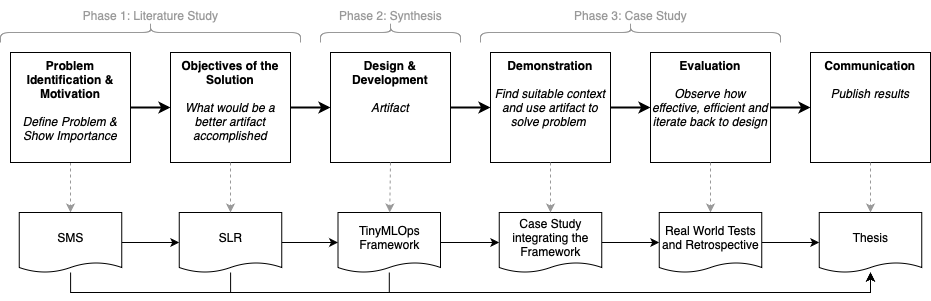
\includegraphics[width=0.975\textwidth]{figs/research_design/dsr-diagramm.png}
    \caption[Research Methodology Overview]{Overview of the Design Science Research approach applied in this study.}
    \label{fig:research-methodology}
\end{figure}

\section{Research Objectives and Questions}
\label{sec:ResearchObjectivesAndQuestions} 

The \glspl{rq} are addressed through a structured methodological approach. Each research phase is designed to progressively refine the understanding of \gls{tinymlops} requirements, best practices, and implementation challenges. RQ1 and RQ2 are primarily addressed through the \gls{sms} and the supplementary \gls{slr} findings. RQ3 is tackled by the conceptual framework design, informed by these literature analyses. Finally, RQ4 is investigated through the case study evaluation of the developed framework. The study is structured around the following \glspl{rq}:

\begin{tabularx}{\textwidth}{@{}lX@{}}
    \textbf{RQ1:} & \emph{What system architectures, methodologies, and practices are employed to support \gls{tinyml} in resource-constrained embedded systems?} \\  
                  & This question examines the current landscape of \gls{tinyml} deployments, analyzing architectural patterns, and design strategies in embedded environments. \\[0.5em]

    \textbf{RQ2:} & \emph{Which frameworks and strategies facilitate decentralized on-device \gls{mlops} while minimizing reliance on cloud infrastructure?} \\  
                  & This question explores methodologies for continuous on-device learning, model retraining, and monitoring in decentralized systems, identifying \gls{lcm} techniques that reduce dependency on cloud-based resources. \\[0.5em]

    \textbf{RQ3:} & \emph{How can a \gls{tinymlops} framework be designed to enable effective on-device model \gls{lcm} in resource-constrained systems?} \\  
                  & Building upon insights from RQ1 and RQ2, this question focuses on the development of a \gls{tinymlops} framework, integrating key methodologies to support model deployment, adaptation, and \gls{lcm}. \\[0.5em]

    \textbf{RQ4:} & \emph{How does deploying on-device TinyMLOps in decentralized embedded systems influence deployment complexity, resource consumption, and performance trade-offs?} \\  
                  & This question shifts the focus from theoretical design to empirical validation, assessing the feasibility of the proposed framework through a case study. It examines deployment complexities, performance trade-offs, and practical constraints that impact real-world implementations. \\  
\end{tabularx}


\section{Literature Analysis Process}
\label{sec:LiteratureReviewProcess}

The literature analysis process commenced with an exploratory search in Google Scholar, employing a broad approach to scan a wide range of publications. This initial step aimed to establish a foundational understanding of key terminologies, emerging research trends, and thematic patterns within \gls{tinymlops} and resource-constrained on-device \gls{ml}. During this phase, three particularly relevant studies were identified. These served as seed papers to refine the research focus and provided key insights that contributed to formulating the initial \glspl{rq} and defining inclusion and exclusion criteria for the subsequent systematic search. Figure~\ref{fig:slr-process} provides an overview of this multi-stage process, outlining the key methodological steps.

\begin{figure}[htbp]
    \centering
    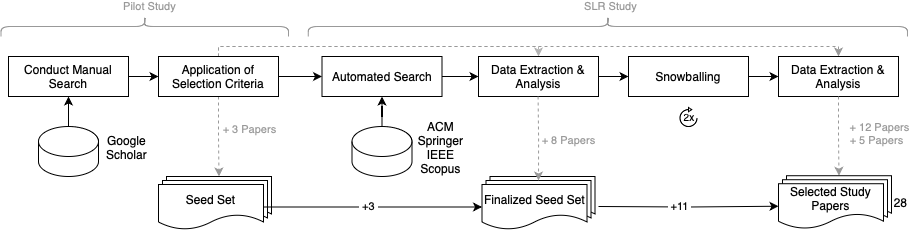
\includegraphics[width=0.975\textwidth]{figs/research_design/SLR-diagramm.png}
    \caption[Systematic Literature Review Process Overview]{Overview of the Systematic Literature Review Process applied in this study.}
    \label{fig:slr-process}
\end{figure}

\subsection{Data Collection}
\label{ssec:data_collection}

While the initial pilot study exclusively relied on Google Scholar, the subsequent systematic search targeted four major literature indexing platforms: ACM Digital Library, SpringerLink, IEEE Xplore, and Scopus. The search strategy was designed to prioritize precision over recall. Such a focus ensured that primarily studies directly relevant to \gls{tinymlops} were included, thereby minimizing the inclusion of irrelevant publications. The final query formulation incorporated key terms such as ``MLOps'' and ``Embedded Machine Learning,'' as detailed in table~\ref{tab:tinymlops-query}.

\begin{table}[htbp]
 \caption[Search Query Structure for TinyMLOps Literature]{Search Query Structure for TinyMLOps Literature.}
\label{tab:tinymlops-query}
\begin{tabularx}{\linewidth}{@{}lL@{}}
\opentableheader
\hl{Query Element} & \hl{Search Terms} \\
\closetableheader
TinyML Domain & ``TinyML'' OR ``Tiny Machine Learning'' OR ``Embedded Machine Learning'' OR ``On-device Machine Learning'' \\
MLOps Domain & ``MLOps'' OR ``Machine Learning Operations'' OR ``Lifecycle Management'' OR ``Operationalization'' OR ``Continuous Training'' OR ``Model Monitoring'' OR ``TinyMLOps'' \\
\bottomrule
\end{tabularx}
\end{table}


\subsection{Application of Selection Criteria}
\label{ssec:selection_criteria}

Following the identification of potentially relevant studies, a manual selection process was conducted based on the inclusion and exclusion criteria. A study was confirmed as a primary source if it satisfied all inclusion criteria and did not meet any exclusion criteria. The selection criteria are detailed in table~\ref{tab:criteria}.

\begin{table}[htbp]
    \caption[Inclusion and Exclusion Criteria for the SLR]{Inclusion and Exclusion Criteria for the Systematic Literature Review.}
    \label{tab:criteria}
    \begin{tabularx}{\linewidth}{@{}lX@{}}
        \opentableheader
        \hl{Criteria Type} & \hl{Description} \\
        \closetableheader
        IC1                & The study addresses \gls{tinyml} concepts, methodologies, or challenges. \\
        IC2                & The study presents practical implementations, experiments, or real-world case studies in the \gls{tinyml} domain, relevant for operations of models. \\
        IC3                & The study addresses lifecycle management characteristics of \gls{ai}-based applications on embedded devices. \\
        \midrule
        EC1                & The study does not meet basic scientific standards (e.g., clear methodology, reproducibility, logical reasoning in conclusions). \\
        EC2                & The study has not undergone peer review or appears in non-reputable sources. \\
        EC3                & The study does not contribute original research or data (e.g., meta-analyses, secondary reviews, purely conceptual discussions without validation). \\
        EC4                & The study was published before 2020. \\
        \bottomrule
    \end{tabularx}
\end{table}

\subsection{Snowballing}
\label{ssec:snowballing}

To enhance the comprehensiveness of the literature mapping and mitigate potential gaps in the automated search results, a bidirectional snowballing process was conducted following Wohlin’s guidelines \cite{wohlinGuidelinesSnowballingSystematic2014a}. This procedure involved both backward snowballing (identifying references cited in selected papers) and forward snowballing (identifying studies that cited the selected papers). Starting with an initial seed set of 11 papers, two iterative rounds of backward and forward snowballing were performed. These iterations led to the inclusion of 17 additional studies after full-text screening. This snowballing process continued until no further relevant studies were identified.

\subsection{Data Extraction}
\label{ssec:data_extraction}

A structured data extraction process was implemented to ensure consistency and traceability across all reviewed studies. For this purpose, a custom extraction template was designed to capture key aspects of the literature. Such aspects were subsequently categorized into five primary dimensions, as detailed in table~\ref{tab:data_extraction_dimensions}.

\begin{table}[htbp]
    \caption[Primary Data Extraction Dimensions]{Primary Data Extraction Dimensions for Literature Analysis.}
    \label{tab:data_extraction_dimensions}
    \begin{tabularx}{\linewidth}{@{}lX@{}}
        \opentableheader
        \hl{Dimension} & \hl{Description} \\
        \closetableheader
        Research Context                & Defines the study’s objective, scope, and classification. \\
        MLOps and Architectural Approaches & Identifies architectural frameworks, \gls{mlops} methodologies, network constraints, and applied technologies. \\
        Hardware and ML Algorithms      & Categorizes hardware platforms and \gls{ml} algorithms used for on-device learning. \\
        Case Studies and Results        & Extracts empirical evidence from real-world deployments or experimental implementations. \\
        Identified Research Gaps        & Assesses limitations discussed, scientific quality considerations, and stated future research directions. \\
        \bottomrule
    \end{tabularx}
\end{table}

To capture characteristics specifically relevant to \gls{tinymlops}, six additional subcategories were defined within the broader dimensions, primarily under ``MLOps and Architectural Approaches'' and ``Hardware and AI Use Case''. The subcategories, listed in table~\ref{tab:tinymlops_subcategories}, facilitated a more granular analysis of the \gls{tinymlops} domain.

\begin{table}[htbp]
    \caption[TinyMLOps-Specific Data Extraction Subcategories]{TinyMLOps-Specific Data Extraction Subcategories.}
    \label{tab:tinymlops_subcategories}
    \begin{tabularx}{\linewidth}{@{}lX@{}}
        \opentableheader
        \hl{Subcategory} & \hl{Description} \\
        \closetableheader
        System Architecture             & Describes the overall system design, including architectural patterns and system behavior. \\
        Runtime Characteristics         & Clusters the runtime environment employed (e.g., compiled, interpreter-based). \\
        Model Training and Optimization & Covers training methodologies (e.g., central, decentralized, hybrid) and model optimization techniques. \\
        Model Management                & Details concepts and practices used for model \gls{lcm} (e.g., versioning, deployment strategies). \\
        CI/CD Practices                 & Clusters automation strategies observed for continuous integration and continuous deployment in the context of \gls{tinyml}. \\
        Monitoring Aspects              & Investigates metrics and strategies utilized for continuous monitoring of models and systems. \\
        \bottomrule
    \end{tabularx}
\end{table}

\subsection{Data Synthesis}
\label{subsec:DataSynthesis}

Following data extraction, a structured synthesis was performed to identify key research trends, technological patterns, and knowledge gaps within \gls{tinymlops}. This synthesis process combined classification techniques, structured mappings, and visual analytics to ensure a comprehensive evaluation of the research landscape. Selected studies were categorized according to research type and contribution type. For research type classification, the method by Wieringa et al. \cite{wieringaRequirementsEngineeringPaper2006} was adopted, distinguishing between solution proposals, validation studies, evaluation studies, philosophical discussions, and experience reports. In parallel, contribution type classification categorized studies based on their outputs, such as frameworks, tools, models, or conceptual insights.

A key component of the synthesis involved mapping \gls{tinymlops} methodologies against hardware constraints. Given the computational limitations of embedded systems, a classification framework was introduced that categorizes hardware based on processing power, memory capacity, and energy efficiency. To further visualize relationships between research domains, methodologies, and technological constraints, multiple mapping studies were conducted employing bubble charts and co-occurrence matrices. Such visualizations enabled a clearer identification of concentrated research areas, emerging trends, and underexplored gaps.

\section{Framework Evaluation Methodology}
\label{sec:FrameworkEvaluationMethodology}

The empirical evaluation of the proposed \gls{tinylcm} framework follows the structured approach outlined by Wohlin et al. \cite{wohlinExperimentationSoftwareEngineering2024}. This methodology ensures a systematic assessment of the framework's feasibility, performance characteristics, and operational constraints under resource-constrained conditions. The evaluation design evolved through iterative refinement, beginning with an ambitious field deployment protocol and culminating in a controlled quasi-experiment that better isolates the framework's core capabilities while maintaining practical relevance.

\subsection{Evolution of the Experimental Design}
\label{ssec:experimental_design_evolution}

Initial planning for the evaluation of \gls{tinylcm} envisioned a series of experiments directly deploying the framework on a battery-powered, mobile Mars rover prototype (a 4tronix kit\footnote{The specific kit used is the 4tronix Mars Rover Robot Kit, further details available at: \url{https://www.elektor.de/products/4tronix-mars-rover-robot-kit-for-raspberry-pi-zero}.} equipped with a Raspberry Pi Zero 2W). The goal was to assess performance, including drift detection, under dynamic conditions across several scenarios involving different object classes and novel ``drift'' objects. However, experiments on this setup revealed significant practical challenges that confounded the ability to isolate and reliably measure the framework's specific contributions:

\begin{itemize}[noitemsep, topsep=0pt]
    \item \textit{Power Instability:} The battery power (four AA alkaline batteries) proved insufficient for sustained operation during computationally intensive phases (camera capture, \gls{tfl} inference, feature processing, and drift monitoring), leading to frequent system shutdowns.
    \item \textit{Hardware Configuration Discrepancies:} Unforeseen differences between the development camera (Pi Camera V2) and the rover's camera (Pi Camera V1.3) introduced variability in image quality and characteristics, impacting model performance.
    \item \textit{Environmental Variability:} Uncontrolled lighting, reflections, and inconsistent object positioning relative to the camera created excessive noise in the data, making it difficult to distinguish genuine concept drift from environmental fluctuations.
    \item \textit{Base Model Performance:} The classification model's accuracy was sometimes insufficient. Misclassifications were potentially misinterpreted as known objects, thus complicating the evaluation of the drift detection mechanisms themselves. This was influenced by both suboptimal model training and environmental variability.
    \item \textit{Timing Mismatch and Data Interpretation:} The experiment initially used a standard system configuration for inference (five frames per second). With objects presented for only two seconds, this led to difficulties in data interpretation, further complicated by the model performance issues, making it hard to determine exact causalities.
    \item \textit{Connectivity and Data Collection Issues:} Unstable SSH connections, due to an unstable network in the laboratory on those days, hindered real-time monitoring and reliable data acquisition during remote rover operation.
\end{itemize}

These limitations underscored the difficulty of conducting rigorous, reproducible experiments in uncontrolled embedded systems. The key lesson learned was the necessity for a more controlled experimental setup to isolate the framework's performance and systematically validate its core functionalities before tackling the full complexity of a dynamic field deployment. This led to the development of a refined experimental design, focusing on controlled laboratory assessments.

\subsection{Experimental Design}
\label{ssec:refined_experimental_design_final}

The refined experimental design aims to systematically evaluate \gls{tinylcm}'s capabilities concerning performance overhead, functional drift detection, and operational robustness on a stationary Raspberry Pi Zero 2W platform. This approach directly supports the investigation of RQ4.

\paragraph{Evaluation Objectives}
The core objectives are to:
\begin{enumerate}[noitemsep, topsep=0pt]
    \item Quantify the computational and memory overhead introduced by \gls{tinylcm}'s components.
    \item Validate the framework's on-device, unsupervised drift detection capabilities under controlled conditions.
    \item Assess system stability and resource utilization during extended operation.
\end{enumerate}

\paragraph{Experiment Hypotheses}
These objectives are translated into the following testable hypotheses:

\begin{tabularx}{\textwidth}{@{}lX@{}}
    \textbf{H$_1$:} & \textit{Performance Overhead:} The computational overhead from \gls{tinylcm} components  increases inference latency by less than 50\% compared to baseline \gls{tfl} inference. This threshold is chosen to ensure that real-time performance, critical for many edge applications, is maintained. \\[0.5em]

    \textbf{H$_2$:} & \textit{Resource Constraints:} The complete \gls{tinylcm} framework operates within defined resource bounds on the target hardware, maintaining average CPU utilization below 50\% (allowing headroom for other system tasks) and memory consumption below \SI{256}{\mega\byte} of the \SI{512}{\mega\byte} available. \\[0.5em]

    \textbf{H$_3$:} & \textit{Drift Detection:} The alarm rate generated by the \gls{tinylcm} framework during periods where untrained (drift) objects are presented is statistically significantly higher than the alarm rate during periods with known objects or background samples. \\
\end{tabularx}

\paragraph{Experimental Setup and Configuration}
All refined quasi-experiments are conducted on a Raspberry Pi Zero 2W, serving as a representative demonstration of a resource-constrained \glspl{sbc}. The key components and configurations of the experimental setup are summarized in Table~\ref{tab:experimental_setup_config}.

\begin{table}[htbp]
    \caption[Refined Experimental Setup and Configuration Details]{Detailed Configuration of the Refined Experimental Setup.}
    \label{tab:experimental_setup_config}
    \begin{tabularx}{\linewidth}{@{}lX@{}} 
        \toprule
        \textbf{Component/Aspect} & \textbf{Specification / Configuration} \\
        \midrule
        Target Hardware & Raspberry Pi Zero 2W \\
        & \textit{SoC:} Broadcom BCM2710A1 (\SI{1}{\giga\hertz} quad-core ARM Cortex-A53) \\
        & \textit{Memory:} \SI{512}{\si{\mega\byte}} LPDDR2 SDRAM \\
        & \textit{Storage:} \SI{32}{\si{\giga\byte}} microSD card \\
        & \textit{Camera:} Raspberry Pi Camera Module V2 (8-megapixel sensor) \\
        \addlinespace 
        Operating System & Raspberry Pi OS Lite (32-bit) \\
        & \textit{Base:} Debian version 12 ``bookworm'' \\
        \addlinespace
        ML Model & MobileNetV2, INT8 quantized (\gls{tfl}) \\ 
        & \textit{Training Data Classes:} ``lego'', ``stone'', ``leaf'', ``negative''. \\
        & \textit{Feature Processing:} L2 Normalization, PCA (1280-D $\rightarrow$ 256-D). \\
        \bottomrule
    \end{tabularx}
\end{table}

The experimental environment is further controlled for lighting (dual artificial sources, no direct sunlight), camera position (fixed at \SI{15}{\centi\meter} from objects), and object placement (defined markings) to ensure consistency across all trials.

\paragraph{Experimental Phases and Scenarios}
The evaluation comprises two main phases:

\textit{Phase 1: Performance Overhead Assessment.} This phase quantifies the computational and memory overhead of \gls{tinylcm} components. It utilizes the three staged configurations previously described: (i) Baseline (\gls{tfl} inference only), (ii) Enhanced Pipeline (\gls{tfl} with feature processing and \gls{knn} classification), and (iii) Complete Framework (full \gls{tinylcm} with drift monitoring).
Each of these three configurations will be executed in five independent runs to account for system variability and enable robust statistical comparisons. Each run will last for a total of \SI{150}{\second}, performing inferences at a rate of five frames per second. The sequence within each run is structured as follows:
\begin{itemize}[noitemsep, topsep=0pt, leftmargin=1em]
    \item \textit{0-30 seconds:} Warm-up period presenting ``negative'' (background) samples. Data from this period will be excluded from performance analysis.
    \item \textit{30-60 seconds:} Presentation of a known object (``lego'').
    \item \textit{60-90 seconds:} Presentation of ``negative'' (background) samples.
    \item \textit{90-120 seconds:} Presentation of a ``drift'' object (``ball'').
    \item \textit{120-150 seconds:} Presentation of ``negative'' (background) samples.
\end{itemize}
Performance metrics (CPU usage, memory consumption, inference latency) will be collected throughout the \SI{120}{\second} following the warm-up period (from seconds 31--150). This phase primarily targets hypotheses H$_1$ and H$_2$.

\textit{Phase 2: Drift Detection Validation.} This phase validates functional drift detection (addressing H$_3$) using two scenarios (Table~\ref{tab:drift_scenarios_refined}) with a reduced frame rate. Known objects are presented for approx. \SI{10}{\second} (5 frames), drift objects for \SI{30}{\second}.

\begin{table}[htbp]
  \caption[Drift Detection Scenarios]{Phase 2 Drift Detection Scenarios (1 inference per 2 seconds).}
  \label{tab:drift_scenarios_refined}
  \begin{tabularx}{\linewidth}{@{}lX@{}}
    \toprule 
    \textbf{Scenario ID} & \textbf{Specification} \\ 
    \midrule 
    S1: Dual Drift & 
      \textit{Trained classes:} ``negative'', ``lego'', ``leaf'', ``stone''. \newline
      \textit{Drift objects (untrained):} ``coin'', ``ball''. \newline
      \textit{Sequence:} neg $\rightarrow$ leaf $\rightarrow$ stone $\rightarrow$ neg $\rightarrow$ lego $\rightarrow$ neg $\rightarrow$ \textbf{ball} $\rightarrow$ neg $\rightarrow$ \textbf{coin} $\rightarrow$ neg $\rightarrow$ lego $\rightarrow$ neg. \\[0.5em]

    S2: Single Drift & 
      \textit{Trained classes:} ``negative'', ``lego'', ``leaf'', ``stone'', ``coin''. \newline
      \textit{Drift object (untrained):} ``ball''. \newline
      \textit{Sequence:} neg $\rightarrow$ leaf $\rightarrow$ stone $\rightarrow$ neg $\rightarrow$ lego $\rightarrow$ neg $\rightarrow$ coin $\rightarrow$ neg $\rightarrow$ \textbf{ball} $\rightarrow$ neg $\rightarrow$ lego $\rightarrow$ neg. \\
    \bottomrule
  \end{tabularx}
\end{table}

\paragraph{Data Collection, Metrics, and Analysis Plan}
Data collection includes automated logging of performance metrics (inference latency, CPU utilization, memory usage) and functional metrics (drift alarm timestamps, confidence scores). Descriptive statistics will characterize the performance. Statistical analyses will be performed using Python with libraries such as SciPy and statsmodels: 

For key quantitative metrics (latency, \gls{cpu} usage, memory usage) derived from the $n=5$ independent runs per configuration, the normality of their distributions will be assessed using the Shapiro-Wilk test \cite{shapiroAnalysisVarianceTest}. The choice between parametric tests (t-tests) and their appropriate non-parametric counterparts will be based on this assessment. A significance level of $\alpha = 0.05$ will be used for all hypothesis testing.

\paragraph{Hypothesis Testing for Performance (H$_1$ and H$_2$)}
The evaluation of performance overhead (H$_1$) and resource constraints (H$_2$) follows the structured plan detailed in Table~\ref{tab:analysis_plan_h1_h2}. The table outlines the specific metrics, statistical tests, and effect size measures used to compare the observed performance against the defined thresholds and to compare the different experimental configurations against each other.

\begin{table}[htbp]
    \caption{Analysis Plan for Performance Hypotheses H$_1$ and H$_2$.}
    \label{tab:analysis_plan_h1_h2}
    \begin{tabularx}{\linewidth}{@{}>{\raggedright\arraybackslash}p{0.07\textwidth} >{\raggedright\arraybackslash}p{0.21\textwidth} >{\raggedright\arraybackslash}X >{\raggedright\arraybackslash}p{0.3\textwidth}@{}}
        \toprule
        \textbf{Hypo\-thesis} & \textbf{Evaluation Metric} & \textbf{Statistical Test} & \textbf{Effect Size Measures} \\
        \midrule
        \textbf{H$_1$} & Inference latency relative to baseline.
        
        \textit{Threshold: < 50\%} & 
        \textit{One-sided one-sample t-test} (if normal) or \textit{one-sided Wilcoxon signed-rank test} (if not normal) to test against the 50\% threshold. &
        The test will be performed on the distribution of latency increases for each configuration. \\
        \addlinespace
        \textbf{H$_2$} & CPU usage. 
        
        \textit{Threshold: < 50\%} & 
        \textit{One-sided one-sample t-test} (if normal) or \textit{one-sided Wilcoxon signed-rank test} (if not normal) to test the distribution of CPU values against the 50\% threshold. & 
        For comparing configurations, \textit{Welch's t-test} or the \textit{Mann-Whitney U test} will be used. Effect size will be quantified using \textit{Cohen's d} or \textit{Cliff's delta}, respectively. \\
        \addlinespace
        \textbf{H$_2$} & Memory consumption. 
        
        \textit{Threshold: < 256 MB} & 
        \textit{One-sided one-sample t-test} (if normal) or \textit{one-sided Wilcoxon signed-rank test} (if not normal) to test the distribution of memory values against the 256 MB threshold. &
        The hypothesis is primarily supported if all values are below the threshold. The statistical test provides additional formal evidence. \\
        \bottomrule
    \end{tabularx}
\end{table}

\paragraph{Hypothesis Testing for Drift Detection (H$_3$)}
The evaluation of drift detection (H$_3$) focuses on assessing the statistical significance of the detection mechanism. The analysis plan, detailed in Table~\ref{tab:analysis_plan_h3}, is designed to determine whether the framework's response to untrained objects is a reliable, non-random event.

\begin{table}[htbp]
    \caption{Analysis Plan for Drift Detection Hypothesis H$_3$.}
    \label{tab:analysis_plan_h3}
    \begin{tabularx}{\linewidth}{@{}>{\raggedright\arraybackslash}p{0.14\textwidth} >{\raggedright\arraybackslash}X >{\raggedright\arraybackslash}p{0.34\textwidth}@{}}
        \toprule
        \textbf{Hypothesis} & \textbf{Metric and Test Condition} & \textbf{Primary Statistical Test and Method} \\
        \midrule
        \textbf{H$_3$} & 
        \textit{Metric:} Proportion of drift alarms.
        
        \textit{Condition:} The alarm rate during ``drift periods'' must be significantly higher than during ``non-drift periods'' ($p < 0.05$). &
        A 2x2 contingency table (Period Type vs. Alarm Triggered) will be created. 
        
        \textit{Fisher's Exact Test} will be used to test for a significant association. \\
        \bottomrule
    \end{tabularx}
\end{table}

\subsection{Threats to Validity}
\label{ssec:evaluation_threats_to_validity}

The refined experimental design aims to mitigate several threats to validity, though some limitations, summarized in Table~\ref{tab:threats_to_validity}, remain.

\begin{table}[htbp]
    \caption[Threats to Validity and Mitigation Strategies for the Refined Experiment]{Threats to Validity and Mitigation Strategies for the Refined Experimental Design.}
    \label{tab:threats_to_validity}
    \begin{tabularx}{\linewidth}{@{}lX@{}}
        \toprule
        \textbf{Threat Category} & \textbf{Description and Mitigation/Acknowledgement} \\
        \midrule
        Internal Validity & 
        \textit{Order effects:} Minimized by consistent system initialization and controlled sequences. The reduced frame rate in Phase 2 also helps ensure consistent temporal object representation. \\
        \addlinespace
        Construct Validity & 
        \textit{Operationalization of ``drift'':} Defined as presentation of untrained object classes. While enabling controlled experiments, this may not fully represent all real-world concept drift complexities. The focus is on detecting statistical feature distribution changes. \\
        \addlinespace
        External Validity & 
        \textit{Hardware generalizability:} Results from the Raspberry Pi Zero 2W offer insights for similar \gls{sbc}s but may not directly transfer to all \gls{mcu}-based platforms or diverse application domains. \newline
        \textit{Environmental realism:} The controlled lab environment, necessary for precision, differs from dynamic field conditions encountered in the initial pilot. \\
        \addlinespace
        Statistical Validity & 
        \textit{Sample size (Phase 1):} Performance data is collected over numerous frames, allowing for robust statistical comparison. \newline
        \textit{Sample size (Phase 2):} The number of distinct drift events per scenario is limited, precluding extensive quantitative generalization of drift detection metrics; hence the focus on qualitative timeline analysis for H$_3$. Effect sizes for performance (H$_1$, H$_2$) will address practical significance beyond p-values. \\
        \bottomrule
    \end{tabularx}
\end{table}


%!TEX root = thesis.tex

\chapter{Results}
\label{chp:Research_Results}

This chapter details findings from systematically investigating the literature, a process outlined in Chapter~\ref{chp:Research_Design} that primarily involved a \gls{sms} augmented by \gls{slr} elements. Section~\ref{sec:GeneralAnalysisResults} first delineates the scope and temporal evolution of the identified literature corpus, demonstrating the emerging nature of \gls{tinymlops} research. Subsequently, section~\ref{sec:QuantitativeFindingsResults} offers a structured classification of the selected publications across multiple dimensions, revealing patterns and research concentrations. Section~\ref{sec:MappingStudiesResults} then synthesizes the interrelationships between key technical aspects. This synthesis consolidates the current state of knowledge and identifies critical research gaps. Finally, Sections~\ref{sec:RQ1_Results_SystemArchitecture} and \ref{sec:RQ2_Results_Frameworks} directly address the first two research questions, drawing upon findings from both the mapping study and the focused literature review.

~\\
\vfill
\minitoc
\clearpage

\section{General Analysis of the Literature Corpus}
\label{sec:GeneralAnalysisResults}

Adhering to the methodology from Section~\ref{sec:LiteratureReviewProcess}, the systematic literature search identified a final corpus of 28 relevant studies published between 2020 and 2024. The selection process, initiated with three seed papers, incorporated a structured database search yielding eight additional studies (query details in Table~\ref{tab:tinymlops-query}) and two subsequent snowballing iterations \cite{wohlinGuidelinesSnowballingSystematic2014a} contributing another twelve and five papers, respectively, as depicted in Figure~\ref{fig:slr-process} (Chapter~\ref{chp:Research_Design}).

The publication distribution, illustrated in Figure~\ref{fig:publication-stats}, reveals a consistent increase in scholarly interest over the analyzed period. Such progressive growth aligns with the growing recognition of \gls{tinymlops} as a distinct research domain, situated at the intersection of \gls{mlops} and resource-constrained computing. From 2022, a notable shift in publication venues occurred: journal articles increasingly supplanted conference proceedings as the primary dissemination medium. This transition may suggest a maturing field, as journal publications typically undergo more extensive peer review and demonstrate greater methodological sophistication. Consequently, the temporal publication pattern indicates \gls{tinymlops}, though relatively new, is rapidly developing in publication volume and scholarly rigor.


\begin{figure}[htbp]
    \centering
    \begin{subfigure}{0.49\textwidth}
        \centering
        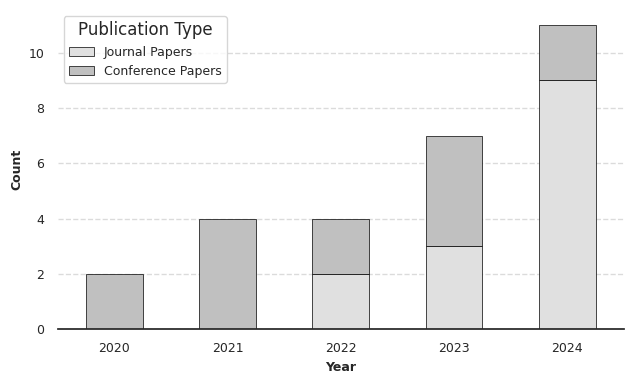
\includegraphics[width=\textwidth]{figs/research_results/publications-stats.png}
        \caption[Publication distribution (2020-2024)]{Distribution of selected publications per year and publication type.}
        \label{fig:publication-stats}
    \end{subfigure}
    \hfill 
    \begin{subfigure}{0.49\textwidth}
        \centering
        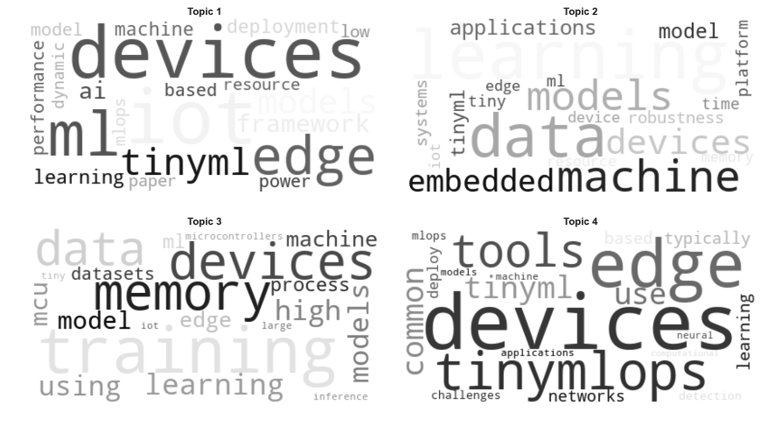
\includegraphics[width=\textwidth]{figs/research_results/topic_modelling.png}
        \caption[Topic modeling of research abstracts]{Topic modeling results from abstracts of the 28 selected papers.}
        \label{fig:TopicModelling}
    \end{subfigure}
    \caption{Temporal and thematic analysis of \gls{tinymlops} research.}
    \label{fig:combined-figures}
\end{figure}

Applying topic modeling to the study abstracts provided deeper insight into thematic patterns, revealing four distinct research clusters (visualized in Figure~\ref{fig:TopicModelling}). The first cluster, Topic 1, centers on the implementation challenges of \gls{ml} deployment on edge devices. Keywords like ``devices'', ``edge'', ``\gls{tinyml}'', and ``perfromance'' highlight resource and energy considerations in \gls{tinyml} applications. In contrast, Topic 2 emphasizes data management within embedded and \gls{iot} environments. This focus is evidenced by the prominence of terms such as ``data'', ``embedded'', ``models'', and ``device'', indicating an emphasis on data-driven adaptation strategies.
The third cluster, Topic 3, addresses the technical constraints of memory utilization and training procedures for \gls{mcu}-based systems. Here, the prevalence of keywords like ``memory'', ``training'', ``model'', and ``\gls{mcu}'' reflects the challenge of executing resource-intensive training operations within severe memory limitations. Finally, Topic 4 concentrates on tooling infrastructure and integrated \gls{mlops} methodologies. Terms including ``tools'', ``\gls{tinymlops}'', ``edge'', and ``device'' signify an emerging focus on comprehensive workflow solutions that address the complexity of model \gls{lcm} in edge computing contexts.

\section{Quantitative Findings from Primary Studies}
\label{sec:QuantitativeFindingsResults}

This section presents a quantitative analysis of the primary studies, examining several dimensions that characterize current \gls{tinymlops} research based on the data extraction framework from Section~\ref{sec:LiteratureReviewProcess}. The analysis proceeds by first exploring research and contribution types (Section~\ref{ssec:ResearchContributionTypeResults}), followed by hardware platforms (Section~\ref{ssec:HardwarePlatformsResults}), \gls{ai} use cases (Section~\ref{ssec:AIUseCaseResults}), system architectures (Section~\ref{ssec:SystemArchitectureResults}), and finally, model training and \gls{lcm} (Section~\ref{ssec:TrainingManagementResults}).

\subsection{Research and Contribution Type}
\label{ssec:ResearchContributionTypeResults}

Following the data synthesis methodology (Section~\ref{subsec:DataSynthesis}), this work classified each publication according to two orthogonal dimensions: research type and contribution type. Research types were categorized using the taxonomy from Wieringa et al. \cite{wieringaRequirementsEngineeringPaper2006}, which distinguishes between solution proposals, validation research, evaluation research, philosophical papers, and experience reports.

\begin{figure}[htbp]
    \centering
    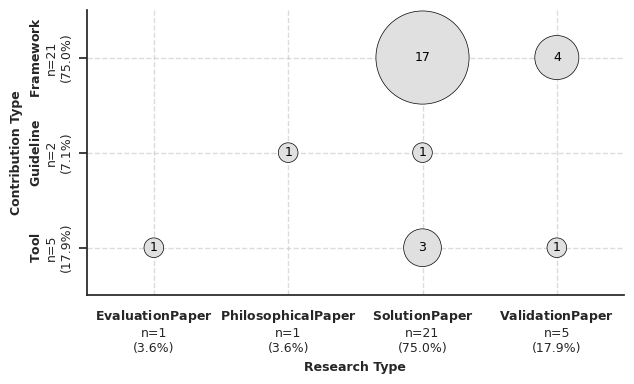
\includegraphics[width=0.8\textwidth]{figs/research_results/contribution-research-type.png}
    \caption[Research and Contribution Type Distribution]{Distribution of \gls{tinymlops} publications by research and contribution type.}
    \label{fig:ResearchContribution}
\end{figure}

Figure~\ref{fig:ResearchContribution} visualizes the distribution of these classifications. The diagram shows 17 publications (approx. 61\%) are solution proposals introducing frameworks, indicating most current research conceptualizes architectural approaches or methodological frameworks for \gls{tinymlops}. Such a focus aligns with the field's nascent state, where researchers establish foundational frameworks to address challenges from resource-constrained environments. In contrast, the lower number of validation studies ($n=5$, approx. 18\%) and evaluation studies ($n=1$, approx. 4\%) suggests a gap in the empirical assessment of proposed solutions. Similarly, the limited presence of guidelines ($n=2$, approx. 7\%) and tooling contributions ($n=5$, approx. 18\%) indicates that the field may not yet have reached a maturity level where comprehensive guidance and standardized toolchains are widely established. This observation aligns with the findings of Kreuzberger et al. \cite{kreuzbergerMachineLearningOperations2023}, who identified similar patterns in the broader \gls{mlops} domain. It suggests that \gls{tinymlops} follows comparable evolutionary trajectories, albeit at an earlier stage of development.
The prevalence of conceptual frameworks ($n=21$, 75\%) coupled with the relative scarcity of empirical validation underscores an imbalance in the current research landscape. More comprehensive real-world validations and longitudinal studies are therefore needed to substantiate the efficacy of proposed \gls{tinymlops} frameworks in production environments.

\subsection{Hardware Platforms and Runtime Environments}
\label{ssec:HardwarePlatformsResults}

Unlike previous reviews with unstructured hardware listings \cite{capogrossoMachineLearningOrientedSurvey2024, rayReviewTinyMLStateoftheart2022, tekinReviewOndeviceMachine2024}, this thesis categorizes platforms based on computational capacity, memory constraints, and operational environment. This classification scheme, presented in Table~\ref{tab:hardware-classification}, distinguishes four primary categories: Ultra-Low-Power, Mid-Range, High-Performance, and \glspl{sbc}.\footnote{The four hardware classes were derived in an iterative session with the OpenAI \textit{ChatGPT} model o1, complemented by targeted web searches (data-sheet specifications and vendor documentation) to anchor the final thresholds in publicly available sources.}

\begin{table}[htbp]
    \caption[Hardware Classification for TinyML Systems]{Hardware Classification for \gls{tinyml} Systems.}
    \label{tab:hardware-classification}
    \begin{tabularx}{\linewidth}{@{}lX@{}}
        \toprule
        \hl{Category}          & \hl{Description} \\
        \midrule
        Ultra-Low-Power        & Clock speed typically below \SI{100}{\mega\hertz}; RAM from a few \gls{kb} to low three-digit \gls{kb} range. \\
        Mid-Range              & Clock speed typically \SIrange{80}{150}{\mega\hertz}; RAM from \SI{32}{\kilo\byte} to \SI{512}{\kilo\byte}. \\
        High-Performance       & Clock speed from approx. \SI{120}{\mega\hertz} to over \SI{600}{\mega\hertz}; RAM from several hundred \gls{kb} up to \SIrange{1}{2}{\mega\byte} on-chip (possibly with additional PSRAM). \\
        Single-Board Computers & Processors such as ARM Cortex-A or similar; run a full OS (e.g., Linux); RAM typically \SI{512}{\mega\byte} or more, often several \gls{gb}. \\
        \bottomrule
    \end{tabularx}
\end{table}

The distribution of hardware platforms across the reviewed literature is depicted in Figure~\ref{fig:hardware-platforms}. High-Performance boards predominate, featured in a majority of studies. This preference suggests that researchers often select devices with sufficient computational capacity for more complex inference tasks, while still aiming for energy efficiency advantages over conventional computing platforms \cite{tekinReviewOndeviceMachine2024}. The second most represented category comprises Mid-Range hardware, which balances computational capability and energy conservation, typically supporting optimized but constrained \gls{ml} models \cite{davidTensorFlowLiteMicro2021}. \Glspl{sbc} constitute a moderate proportion of the studied platforms; implementations frequently leverage multi-process capabilities of conventional operating systems or specialized hardware accelerators (e.g., TPUs, GPUs) \cite{tekinReviewOndeviceMachine2024}. In contrast, Ultra-Low-Power devices receive comparatively limited attention, reflecting the trade-off between minimal energy consumption and computational feasibility for \gls{ml} workloads.

Among specific hardware implementations, the Raspberry Pi 4 Model 4B and the Arduino Nano 33 BLE each appear in five studies (approx. 18\%), while the nRF52840 board is featured in four publications (approx. 14\%). This concentration may indicate the emergence of de facto standard platforms for \gls{tinyml} research and development.
Complementing the hardware analysis, Figure~\ref{fig:runtime-env} illustrates the distribution of runtime environments. Approximately half of the reviewed implementations ($n=15$, approx. 54\%) utilize compiled runtimes to maximize performance. While such approaches optimize execution latency for inference, they can introduce complexity for frequent model updates \cite{banburyEdgeImpulseMLOps2023}. This trade-off becomes critical in production environments where model evolution necessitates streamlined update mechanisms \cite{lootusVMContainerizedApproach2022}. Interpreter-based environments ($n=12$, approx. 43\%) predominantly employ MicroPython implementations. Despite generally lower performance, these environments offer flexibility through lightweight bytecode execution and specialized numerical libraries \cite{antoniniTinyMLOpsFrameworkOrchestrating2022}. The limited representation of \gls{onnx}-based runtimes ($n=2$, approx. 7\%) suggests that vendor-specific inference engines continue to dominate the \gls{tinyml} landscape. Broader adoption of standardized interchange formats like \gls{onnx} could enhance model portability and deployment flexibility, albeit potentially requiring adaptations to existing toolchains \cite{fraidlingTinyMachineLearning2023}.

\begin{figure}[htbp]
    \centering
    \begin{subfigure}{0.64\textwidth}
        \centering
        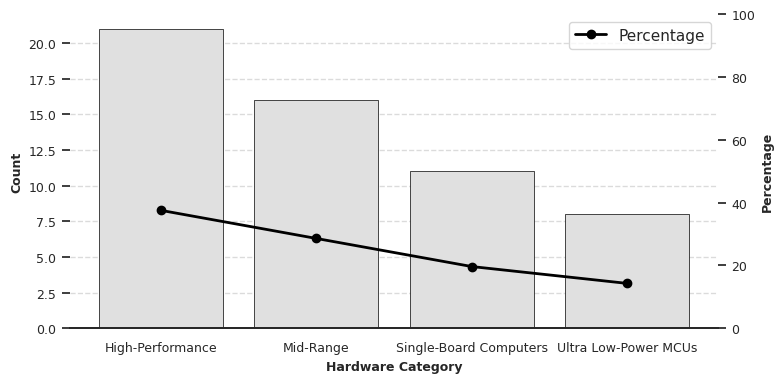
\includegraphics[width=\textwidth]{figs/research_results/hardware-platforms.png}
        \caption[Hardware platform distribution]{Distribution of hardware platforms in reviewed studies.}
        \label{fig:hardware-platforms}
    \end{subfigure}
    \hfill
    \begin{subfigure}{0.34\textwidth}
        \centering
        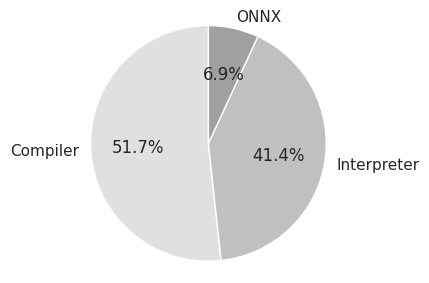
\includegraphics[width=\textwidth]{figs/research_results/runtime.png}
        \caption[Runtime environment distribution]{Runtime environment usage in reviewed studies.}
        \label{fig:runtime-env}
    \end{subfigure}
    \caption{Hardware platforms and runtime environments in \gls{tinymlops} implementations.}
    \label{fig:hardware-vs-runtime}
\end{figure}

\subsection{AI Use Cases and Data Modalities}
\label{ssec:AIUseCaseResults}

To identify primary application domains, the literature corpus was analyzed according to \gls{ai} tasks and corresponding input data modalities. Figure~\ref{fig:ai-use-cases} summarizes the principal \gls{ai} domains. Computer Vision applications constitute one-third of documented use cases (33\%, $n \approx 9$)\footnote{Percentages for AI use cases and data types are based on counts of application instances, where a single paper may report multiple use cases or data types, leading to adjusted counts if summed directly from $N=28$ papers. The text reports proportions based on the total number of identified instances.}, encompassing tasks such as object detection, classification, and segmentation (e.g., \cite{azevedoDetectingFaceMasks2023a}, a face mask detection system on ultra-low-power \glspl{mcu}). Audio Processing represents approximately 20\% of implementations ($n \approx 5$), with keyword spotting and acoustic scene analysis being prevalent (e.g., \cite{grauOnDeviceTrainingMachine2021}). Sensor-based Analysis is the largest category, comprising nearly half of use cases (47\%, $n \approx 13$), and includes diverse applications like anomaly detection, time-series forecasting, and environmental monitoring (e.g., an industrial anomaly detection system \cite{antoniniTinyMLOpsFrameworkOrchestrating2022}). For a more granular understanding, Appendix~\ref{app:detailed-ai-use-cases} provides a detailed breakdown of specific use cases via Figure~\ref{fig:detailed-ai-use-cases}.

\begin{figure}[htbp]
    \centering
    \begin{subfigure}{0.49\textwidth}
        \centering
        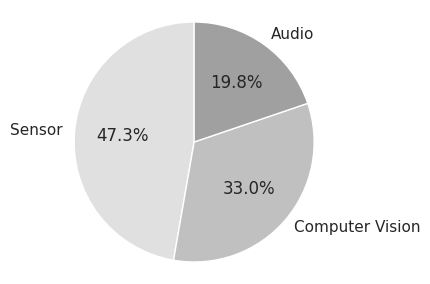
\includegraphics[width=\textwidth]{figs/research_results/sms_used_ai_type.png}
        \caption[AI use case distribution]{Distribution of AI use cases.}
        \label{fig:ai-use-cases}
    \end{subfigure}
    \hfill
    \begin{subfigure}{0.49\textwidth}
        \centering
        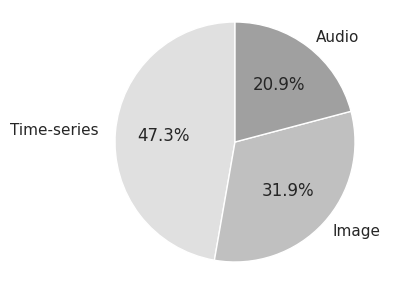
\includegraphics[width=\textwidth]{figs/research_results/sms_used_input_data_type.png}
        \caption[Input data type distribution]{Distribution of input data types.}
        \label{fig:input-data}
    \end{subfigure}
    \caption{AI applications and input data types in \gls{tinymlops} research.}
    \label{fig:ai-use-case-vs-input}
\end{figure}

The distribution of input data types, illustrated in Figure~\ref{fig:input-data}, corroborates the application domain analysis. Time-series data represents nearly half of the studied implementations (47\%, $n \approx 13$), aligning with the prevalence of sensor-driven analytics. Image data accounts for approximately one-third of cases (32\%, $n \approx 9$), corresponding to vision-oriented applications. Audio data completes the distribution at roughly 21\% ($n \approx 6$), reflecting the deployment of on-device speech recognition and acoustic analysis systems.

This categorization of \gls{ai} use cases provides context for addressing RQ3 (from Section~\ref{sec:ResearchObjectivesAndQuestions}). The predominance of sensor-based applications suggests that \gls{tinymlops} frameworks should prioritize efficient processing of time-series data and accommodate operational patterns of continuous sensor monitoring.

\subsection{System Architecture Patterns}
\label{ssec:SystemArchitectureResults}

Figure~\ref{fig:sysAarch} demonstrates the distribution of system architecture patterns that the surveyed articles present. Although the \gls{tinymlops} paradigm inherits many established \gls{devops} and \gls{mlops} workflows, it typically requires specialized optimizations for resource-constrained deployments.

\begin{figure}[htbp]
    \centering
    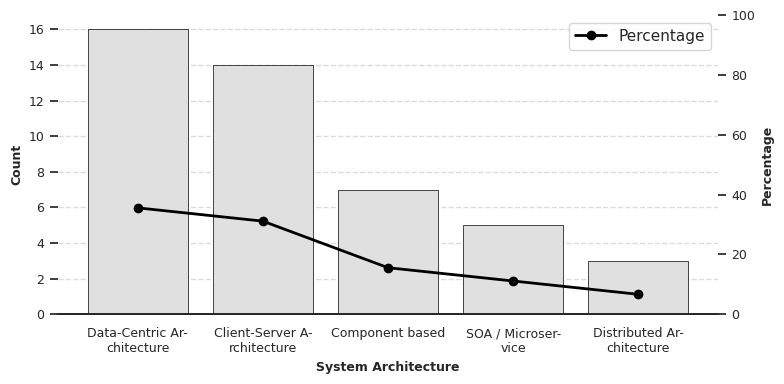
\includegraphics[width=0.975\textwidth]{figs/research_results/sms-system-architecture.png}
    \caption[Distribution of system architecture patterns]{Distribution of system architecture patterns in \gls{tinymlops} literature.}
    \label{fig:sysAarch}
\end{figure}

Data-Centric Architectures lead with a 36\% share ($n=16$ of 45 architectural instances counted across papers)\footnote{Architectural pattern counts may exceed the number of papers (28) as some studies discuss or implement multiple architectures.}, emphasizing refined data pipelines for preprocessing, retraining, and incremental updates \cite{rajEdgeMLOpsAutomation2021, leTinyMLOpsRealtimeUltralow2023a}. Client-Server Architectures follow at 31\% ($n=14$), indicating that numerous \gls{tinyml} solutions remain partially reliant on cloud-based resources \cite{minSensiXBringingMLOps2023, fraidlingTinyMachineLearning2023}. Furthermore, 16\% of instances ($n=7$) implement Component-Based approaches that encapsulate independent functionalities for more agile updates. In contrast, only 11\% ($n=5$) rely on SOA/Microservices, possibly due to overheads from microservice decomposition on highly resource-constrained devices. Distributed Architectures occur in a minimal 7\% of instances ($n=3$), often in the context of  \gls{fl}, which was not a primary focus in most reviewed studies and thus appears underrepresented. Consequently, \gls{tinyml} architectures frequently adapt high-level \gls{mlops} principles—particularly data processing flows—to device-limited contexts. As pragmatic choices, these architectures predominantly use data-centric or hybrid cloud-edge topologies.

\subsection{Model Training and Lifecycle Management}
\label{ssec:TrainingManagementResults}

Addressing model adaptability and \gls{lcm} is pivotal in \gls{tinymlops}. Figure~\ref{fig:training-learning-vs-lcm} illustrates key findings regarding model training approaches (Figure~\ref{fig:training-learning}) and the extent to which studies address \gls{lcm} (Figure~\ref{fig:lcm-done}).

Model Training was classified into three categories based on the location and dependency of the training process \cite{capogrossoMachineLearningOrientedSurvey2024}:

\begin{itemize}[noitemsep, topsep=0pt]
    \item \textit{Central Training}: The \gls{ml} model is trained primarily in a cloud or centralized infrastructure. This method involves data transfer from edge devices to a central server, followed by deployment of the trained model to edge devices.
    \item \textit{Decentral Training}: Training occurs directly on the edge device, without primary reliance on cloud infrastructure. This enables on-device learning and adaptation to local data while reducing cloud dependencies.
    \item \textit{Hybrid Training}: Combines central and decentralized training approaches. This may involve initial training in a central environment, followed by on-device fine-tuning or incremental updates.
\end{itemize}

Model Learning Type was categorized based on the model's adaptation behavior during operation:
\begin{itemize}[noitemsep, topsep=0pt]
    \item \textit{Offline Learning}: The model is trained as a static entity before deployment. No further updates occur during operation \cite{capogrossoMachineLearningOrientedSurvey2024}.
    \item \textit{Online Learning}: The model continuously updates during operation, adapting to newly encountered data \cite{renOndeviceOnlineLearning2024}.
    \item \textit{Incremental Learning}: The model undergoes periodic updates, improving based on new but limited datasets while maintaining prior knowledge \cite{disabatoIncrementalOnDeviceTiny2020}.
\end{itemize}

\begin{figure}[htbp]
    \centering
    \begin{subfigure}{0.62\textwidth}
        \centering
        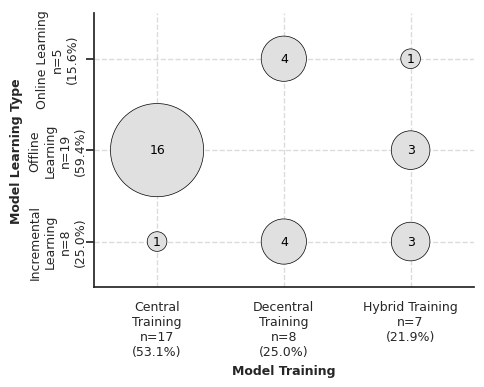
\includegraphics[width=\textwidth]{figs/research_results/sms-training-ort.png}
        \caption[Model training vs. learning type]{Cross-tabulation of training location with learning type.}
        \label{fig:training-learning}
    \end{subfigure}
    \hfill 
    \begin{subfigure}{0.36\textwidth}
        \centering
        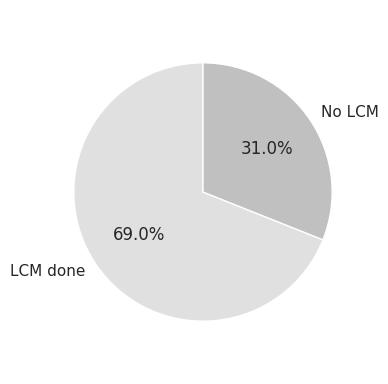
\includegraphics[width=\textwidth]{figs/research_results/lcm-done.png}
        \caption[LCM application in studies]{Share of studies addressing \gls{lcm} practices.}
        \label{fig:lcm-done}
    \end{subfigure}
    \caption{Training approaches and lifecycle management in \gls{tinymlops}.}
    \label{fig:training-learning-vs-lcm}
\end{figure}

Figure~\ref{fig:training-learning} suggests that over half of the examined studies ($n=17$, approx. 53\%) employ Central Training. Nearly all of these ($n=16$) are paired with Offline Learning, indicating a strong preference for pre-trained, static models deployed to edge devices. Although Decentralized Training represents about a quarter of approaches ($n=8$, approx. 25\%), such efforts often emphasize Online Learning ($n=4$) or Incremental Learning ($n=4$), catering to scenarios where on-device model adaptation is essential. Hybrid Training ($n=7$, approx. 22\%) introduces transitional solutions, such as training large base models in the cloud and then fine-tuning or updating incrementally on edge devices. However, given the relatively small number of hybrid-training papers, further validation of these techniques is warranted.

Likewise, Figure~\ref{fig:lcm-done} shows that approximately 69\% of studies ($n=19$) address \gls{lcm}. These articles discuss long-term performance monitoring, redeployment strategies, versioning systems for embedded models, and other operational considerations vital for reliability \cite{huangRIOTMLToolkitOvertheair2024a, sudharsanOTATinyMLAirDeployment2022}. Nonetheless, about 31\% of studies ($n=9$) do not cover \gls{lcm} at all. This potentially leaves open questions regarding safe and resilient continuous deployment for \gls{tinyml} systems across their entire operational lifecycle.

Overall, these findings indicate a continued tendency toward statically trained models for small edge devices. Yet, the potential for real-time or local adaptation in \gls{tinyml} is fostering research on more dynamic training paradigms and a clearer emphasis on the entire lifecycle, bridging initial development, deployment, and ongoing maintenance.

\section{Mapping Studies of Interdependencies}
\label{sec:MappingStudiesResults}

To further elucidate interdependencies within the \gls{tinymlops} landscape, this section builds upon the preceding findings by presenting detailed cross-tabulation analyses. These multi-dimensional mappings explore relationships between aspects such as system architecture, hardware, model training (Section~\ref{ssec:ArchitectureHardwareTrainingResults}), management practices (Section~\ref{ssec:ArchitectureTrainingManagementResults}, Section~\ref{ssec:ManagementLearningMonitoringResults}), CI/CD tactics with optimization techniques (Section~\ref{ssec:CICDTrainingOptimizationResults}), and finally, hardware platforms with \gls{ai} use cases (Section~\ref{ssec:HardwareAIUseCasesResults}). The goal is to reveal complex patterns not apparent from single-dimension analyses, offering deeper insights into current research configurations.

\subsection{Interplay of Architecture, Hardware, and Model Training}
\label{ssec:ArchitectureHardwareTrainingResults}

Figure~\ref{fig:bubble-chart-arch-hw-training} illustrates the distribution of studies across these three dimensions, with bubble size representing frequency. Hardware platforms follow the taxonomy from Table~\ref{tab:hardware-classification}, while system architectures and model training approaches correspond to classifications in Sections~\ref{ssec:SystemArchitectureResults} and \ref{ssec:TrainingManagementResults}.

\begin{figure}[htbp]
    \centering
    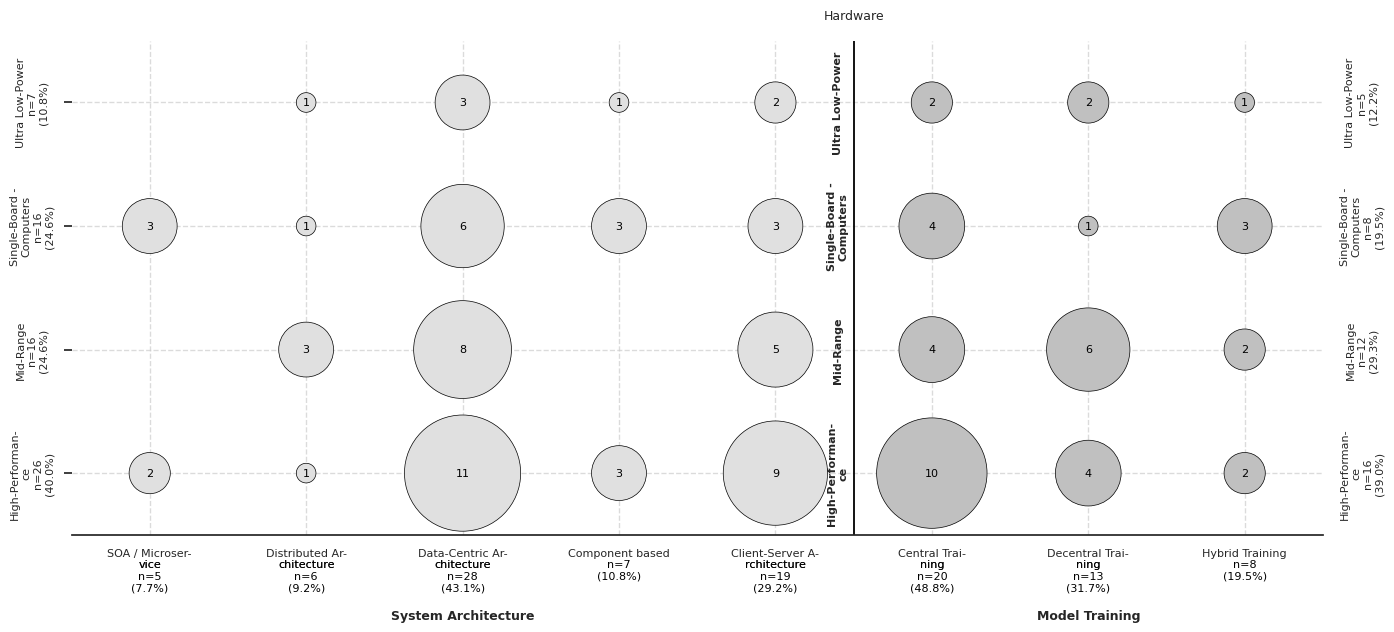
\includegraphics[width=1\textwidth]{figs/research_results/sms_archi-training-hardware.png}
    \caption[Mapping of System Architecture, Hardware, and Training]{Relationship between system architecture, hardware platform, and model training in \gls{tinymlops} implementations.}
    \label{fig:bubble-chart-arch-hw-training}
\end{figure}

Analyzing System Architecture and Hardware Platform dimensions reveals distinct pairing preferences. Data-Centric Architectures are predominant in High-Performance ($n=11$) and Mid-Range Hardware ($n=8$) implementations, appearing less frequently in \glspl{sbc} ($n=6$) and Ultra-Low-Power Hardware ($n=3$). This distribution suggests data-centric approaches are viable across the hardware spectrum but gravitate towards more capable platforms, likely reflecting computational demands of comprehensive data processing.
Similarly, Client-Server architectures appear most frequently with High-Performance ($n=9$) and Mid-Range Hardware ($n=5$), with modest representation in \glspl{sbc} ($n=3$) and Ultra-Low-Power boards ($n=2$).
Conversely, Distributed Architectures concentrate primarily in Mid-Range ($n=3$) and Ultra-Low-Power ($n=1$ instance) categories, with minimal representation in high-performance contexts. This pattern reflects the specialized nature of distributed architectures within \gls{tinymlops}, often tied to \gls{fl} implementations \cite{grauOnDeviceTrainingMachine2021}. The limited overall presence of distributed approaches stems from the study's scope rather than indicating irrelevance to the broader field.\footnote{The discrepancy in Distributed Architecture counts compared to Section~\ref{ssec:SystemArchitectureResults} arises because individual studies often evaluate multiple hardware configurations while maintaining a consistent architectural approach.}
SOA/Microservices approaches manifest infrequently overall. When employed, they cluster with High-Performance Hardware ($n=2$) and \glspl{sbc} ($n=3$), with no presence in Mid-Range or Ultra-Low-Power categories. This distribution suggests the inherent overhead of microservice architectures restricts their deployment to edge devices with substantial computational resources \cite{rajEdgeMLOpsAutomation2021}. A comparable distribution characterizes Component-Based Architectures, appearing relatively evenly across High-Performance Hardware ($n=3$) and \glspl{sbc} ($n=3$), but diminishing considerably in mid-range and ultra-low-power categories

Regarding the relationship between hardware platforms and training methodologies, Central Training approaches cluster predominantly with High-Performance ($n=10$), Mid-Range ($n=4$), and \glspl{sbc} ($n=4$). This confirms a trend of cloud-based training being common across various capable hardware categories.
In contrast, Decentralized Training strategies are more distributed, appearing most with Mid-Range hardware ($n=6$), followed by High-Performance ($n=4$), with fewer implementations in Ultra-Low-Power ($n=2$) and \glspl{sbc} ($n=1$). This pattern indicates on-device training is gaining traction even in moderately constrained environments.
Hybrid Training configurations span diverse hardware, with a relative concentration in \gls{sbc} implementations ($n=3$ studies) and High-Performance ($n=2$). This suggests hybrid approaches may balance edge autonomy with computational feasibility, such as solutions leveraging pre-trained feature extractors with locally adaptable classification layers \cite{disabatoIncrementalOnDeviceTiny2020}.

Cross-referencing these analyses unveils a significant cluster around Client-Server and Data-Centric Architectures on High-Performance boards using Central Training. This recurring pattern signals a preference for these architectures on capable edge platforms while offloading intensive training to cloud infrastructure (e.g., \cite{banburyEdgeImpulseMLOps2023}). Furthermore, this configuration underscores the relationship between client-server architectures and cloud services beyond model training, as demonstrated in frameworks for collaborative inference \cite{antoniniTinyMLOpsFrameworkOrchestrating2022}. Broader findings also indicate that while ultra-low-power implementations exist, their integration within dominant high-performance paradigms remains sparse, suggesting relevance primarily in specialized applications prioritizing extreme energy efficiency \cite{pavanTyBoxAutomaticDesign2024}.
Overall, the mapping reveals that while central training is predominant, training methodology selection is not strictly determined by hardware tier. It reflects a complex interplay of factors, including the ongoing exploration of decentralized and hybrid approaches across the \gls{tinymlops} spectrum.

\subsection{Interplay of Architecture, Training, and Model Management}
\label{ssec:ArchitectureTrainingManagementResults}

Expanding on the hardware-centric analysis (Section~\ref{ssec:ArchitectureHardwareTrainingResults}), this subsection incorporates Model Management practices for a more comprehensive perspective on operational patterns. Figure~\ref{fig:bubble-chart-arch-training-mgmt} visualizes the distribution of primary studies across System Architecture, Model Training methodologies, and Model Management practices.

\begin{figure}[htbp]
    \centering
    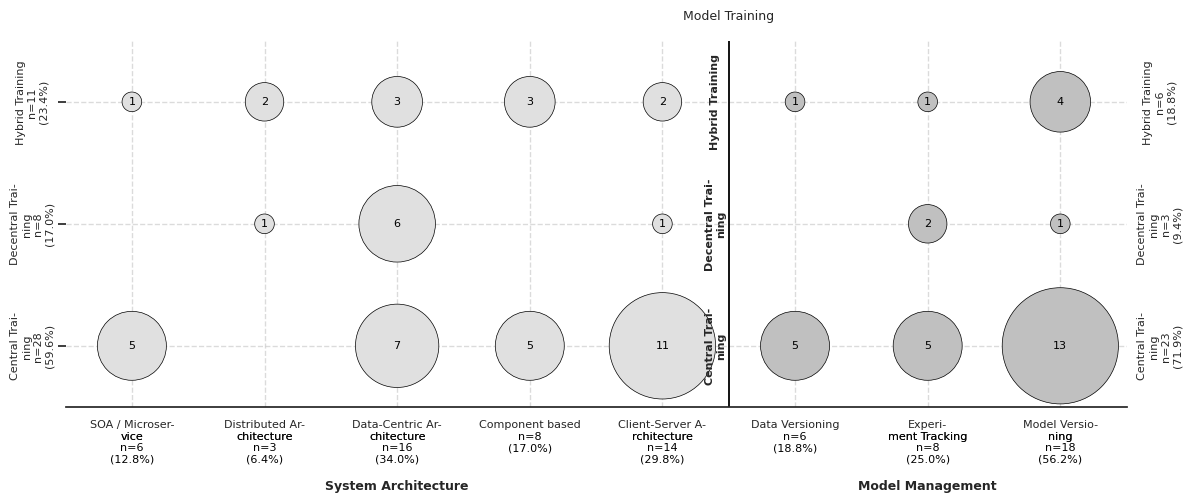
\includegraphics[width=1\textwidth]{figs/research_results/sms_archi-training-lcm.png}
    \caption[Mapping of System Architecture, Training, and Management]{Correlation between system architecture, model training, and model management practices.}
    \label{fig:bubble-chart-arch-training-mgmt}
\end{figure}

Mapped relationships confirm that SOA/Microservices and Distributed Architectures, consistent with their limited overall presence (Section~\ref{ssec:ArchitectureHardwareTrainingResults}), show minimal representation across management and training combinations. Proportionally, SOA/Microservices architectures show an almost exclusive affinity with Central Training ($n=5$). A similar pattern emerges for Component-Based architectures ($n=5$ with Central Training, $n=3$ with Hybrid). These correspondences suggest implementing microservice-based and component-based architectures often involves cloud infrastructure for model training. Such configurations typically occur within larger, complex systems where cloud integration and sophisticated tooling are prevalent \cite{fraidlingTinyMachineLearning2023}. This aligns with Section~\ref{ssec:ArchitectureHardwareTrainingResults}, where both architectural approaches appeared less frequently, likely due to resource demands in constrained environments.
Distributed Architectures show sparse representation, particularly with hybrid and decentralized training. This aligns with \gls{fl} principles, where models train on edge devices, with only weight updates transmitted centrally.
Data-Centric Architectures, while prevalent across all training methodologies, display a modest concentration with Central Training ($n=7$) alongside considerable presence with Decentral Training ($n=6$). This balance underscores the versatility of data-centric approaches for diverse training paradigms, from cloud-based batch learning to adaptive on-device techniques.
In contrast, Client-Server Architectures demonstrate a pronounced preference for Central Training ($n=11$), reinforcing their reliance on robust, centralized training infrastructure—a pattern consistent with hardware associations in Section~\ref{ssec:ArchitectureHardwareTrainingResults}.

Shifting focus to Model Management techniques and their relationship with training methodologies reveals additional patterns. Within the corpus, Model Management practices include Data Versioning ($n=6$, approx. 19\%), Experiment Tracking ($n=8$, approx. 25\%), and Model Versioning ($n=18$, approx. 56\%). Among these, Model Versioning is the predominant practice across all training approaches, with particular dominance alongside Central Training ($n=13$). This strong association reflects the established \gls{mlops} emphasis on rigorous model version control in centralized development.
Experiment Tracking similarly gravitates toward Central Training ($n=5$) but also appears with decentralized ($n=2$) and hybrid ($n=1$) approaches, suggesting broader applicability. Notably, while model versioning predominates overall, experiment tracking appears proportionally more frequent in decentralized contexts.\footnote{One might postulate that Experiment Tracking and Model Versioning are typically employed in tandem, particularly in Decentral Training. However, this does not appear to be the case within reviewed studies. This observation might stem from \gls{fl} emphasis on transmitting model weights rather than explicit versioning. Definitive confirmation requires additional research given the limited number of \gls{fl} papers in this study.}
Data Versioning, though less common, also concentrates primarily with Central Training ($n=5$). This suggests robust data management practices feature predominantly in centralized \gls{tinyml} pipelines, aligned with established data-centric \gls{mlops} workflows.

Collectively, these mappings highlight that Central Training not only remains the prevailing paradigm in \gls{tinymlops} but also shows substantial integration with established \gls{mlops} practices like Model Versioning and Experiment Tracking. The convergence of Client-Server Architecture, Central Training, and Model Versioning represents a predominant configuration: leveraging client-server topologies with cloud-based training while implementing rigorous model version control. This reinforces the pattern from Section~\ref{ssec:ArchitectureHardwareTrainingResults}, where client-server architectures frequently paired with high-performance hardware and central training, indicating a consistent architectural approach.
Nevertheless, the emerging presence of Decentral Training and Hybrid Training alongside Experiment Tracking signals an incipient shift toward more agile, on-device \gls{mlops} practices, though still in early developmental stages. This nascent trend, while not yet predominant, potentially represents an evolving research direction addressing centralized training limitations in increasingly autonomous edge scenarios.

\subsection{Interplay of Management, Learning, and Monitoring}
\label{ssec:ManagementLearningMonitoringResults}

Deepening the dimensional analysis, this subsection investigates interrelationships between Model Management practices, Model Learning types, and Monitoring metrics. This offers granular insights into \gls{tinymlops} operational dynamics. Figure~\ref{fig:bubble-chart-mgmt-learning-monitoring} visualizes the distribution of primary studies across these dimensions, complementing preceding analyses of architecture, hardware, and training.

The analysis first considers the relationship between Model Management techniques and Model Learning Types. Model Management practices comprise Model Versioning ($n=21$, approx. 57\%), Experiment Tracking ($n=10$, approx. 27\%), and Data Versioning ($n=6$, approx. 16\%). Monitoring metrics include Model Accuracy ($n=23$, approx. 33\%), Concept/Data Drift ($n=19$, approx. 27\%), Computational Latency ($n=18$, approx. 26\%), and RAM Usage ($n=10$, approx. 14\%). Consistent with patterns in Section~\ref{ssec:TrainingManagementResults}, Offline Learning predominates, followed by Incremental Learning and Online Learning.

\begin{figure}[htbp]
    \centering
    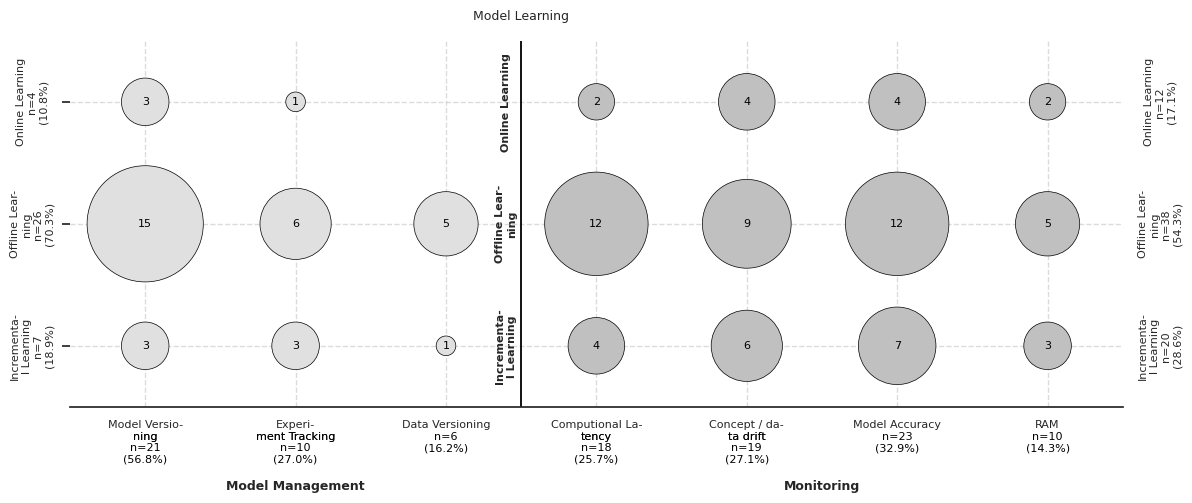
\includegraphics[width=1\textwidth]{figs/research_results/sms-learning-monitoring.png}
    \caption[Mapping of Model Management, Learning, and Monitoring]{Integration of model management, learning types, and monitoring metrics in \gls{tinymlops} systems.}
    \label{fig:bubble-chart-mgmt-learning-monitoring}
\end{figure}

Examination of mapped relationships reveals that Model Versioning, while prominent across all learning categories, converges markedly with Offline Learning ($n=15$). This pairing reinforces the established \gls{mlops} emphasis on version control for statically trained models, aligning with the broader tendency toward centralized training and offline deployment.
Experiment Tracking, though less frequent, similarly gravitates toward Offline Learning ($n=6$) while maintaining some presence with Incremental Learning ($n=3$) and Online Learning ($n=1$). This pattern suggests experiment tracking's applicability across learning paradigms, though still predominantly in offline contexts.
Data Versioning, the least common management practice, also concentrates primarily with Offline Learning ($n=5$), indicating that explicit data management typically accompanies static, pre-deployment training workflows.

The secondary mapping examines Monitoring Metrics in relation to Model Learning Types. Model Accuracy and Computational Latency monitoring strongly associate with Offline Learning ($n=12$ for both). These dual concentrations highlight practical priorities for offline learning: ensuring high model performance and efficient inference on resource-constrained hardware.
Concept/Data Drift monitoring, while slightly less prevalent, shows notable correlation with Incremental Learning ($n=6$). This association indicates drift detection's relevance for adaptive models undergoing periodic updates that must maintain performance in evolving environments.
RAM Usage, the least common monitoring metric, distributes relatively uniformly across learning types. This suggests memory consumption is a device-level concern spanning different learning paradigms rather than being specifically emphasized by one approach.

Collectively, these mappings reinforce the overarching pattern that Offline Learning and Central Training remain predominant. They show strong connections to established practices like Model Versioning and a dual focus on Model Accuracy and Computational Latency as primary performance indicators.
Notably, while Experiment Tracking and Data Versioning appear less frequently, their associations with Offline Learning suggest conventional \gls{tinymlops} workflows are beginning to incorporate elements of systematic experimentation and data management. Interestingly, monitoring metrics, when analyzed proportionally to each learning type, distribute relatively evenly across different approaches and management practices. This balanced distribution indicates monitoring is a fundamental aspect of \gls{tinymlops}, regardless of specific learning or management strategy. Whether implementing static, pre-trained models or adaptive, on-device learning, continuous assessment of performance, resource utilization, and phenomena like concept drift remains essential for reliability, efficiency, and operational longevity. This widespread recognition of monitoring's importance may signal the \gls{tinymlops} field's maturation toward more comprehensive operational practices beyond initial model development and deployment, reflecting an increasing emphasis on full \gls{lcm}.

\subsection{Interplay of CI/CD, Training, and Optimization}
\label{ssec:CICDTrainingOptimizationResults}

Building upon previous dimensional analyses, this subsection explores interrelationships between \gls{ci}/\gls{cd} tactics, Model Training methodologies, and Optimization techniques. This provides deeper insights into deployment and efficiency considerations. Figure~\ref{fig:bubble-chart-cicd-training-optimization} visualizes the distribution of primary studies across these dimensions. Detailed descriptions of \gls{ci}/\gls{cd} tactics and optimization techniques can be found in Table~\ref{tab:cicd-optim-techniques} (Appendix).

The mapping first examines \gls{ci}/\gls{cd} Tactics in relation to Model Training types. Within the corpus, \gls{ci}/\gls{cd} tactics comprise Automated Deployment and Full Model Update (both $n=20$, approx. 37\%), followed by Partial Model Update ($n=11$, approx. 20\%) and Automated Tests ($n=3$, approx. 6\%). Optimization Techniques include Quantization and Pruning ($n=17$, approx. 57\%), Test-Time Adaptation and Adaptive Computation (both $n=4$, approx. 13\% each), Feature Caching ($n=3$, 10\%), and Knowledge Distillation ($n=2$, approx. 7\%).

\begin{figure}[htbp]
    \centering
    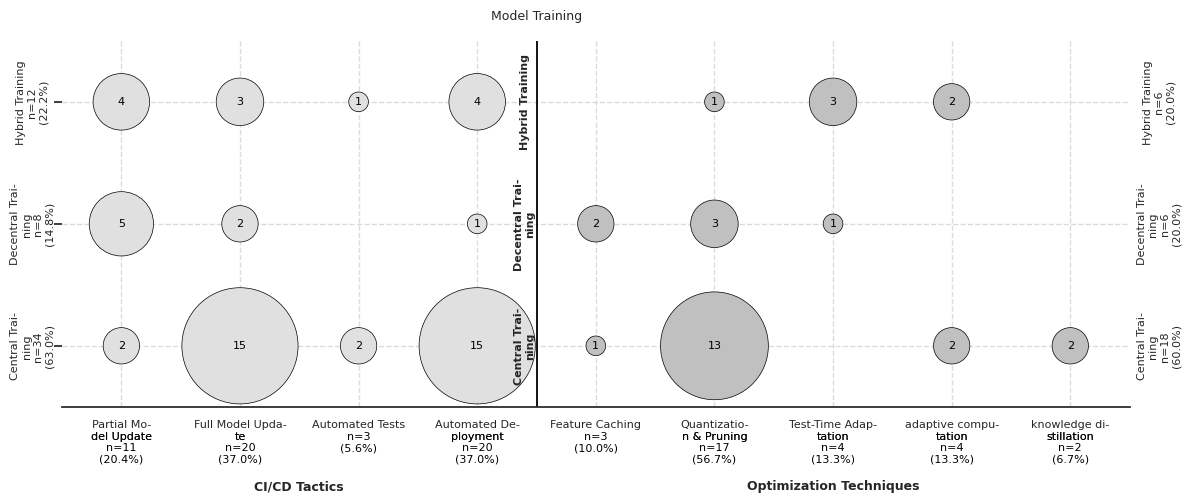
\includegraphics[width=1\textwidth]{figs/research_results/sms_cicd-training-optimization.png} 
    \caption[Mapping of CI/CD Tactics, Training, and Optimization]{CI/CD tactics in relation to model training and optimization techniques.}
    \label{fig:bubble-chart-cicd-training-optimization}
\end{figure}

Analysis of mapped relationships reveals a significant convergence of Full Model Update with Central Training ($n=15$). This association indicates the predominant \gls{ci}/\gls{cd} approach involves complete model replacement within centralized training workflows.
In contrast, Partial Model Update displays a more balanced distribution across Decentral Training ($n=5$) and Hybrid Training ($n=4$). This suggests incremental updates feature more prominently in on-device or hybrid learning contexts where efficient adaptation to new data takes precedence over complete retraining.
Automated Deployment, paralleling Full Model Update, shows strong correlation with Central Training ($n=15$), reinforcing reliance on automated deployment pipelines for centrally trained models.
Automated Tests, though infrequently mentioned as a \gls{ci}/\gls{cd} tactic, also primarily associate with Central Training ($n=2$). This indicates automated testing practices, where present, typically integrate into established, cloud-centric \gls{mlops} workflows alongside full model updates.

The secondary mapping examines Optimization Techniques in relation to Model Training types. This analysis reveals a marked predominance of Quantization and Pruning with Central Training ($n=13$). This strong association underscores that these techniques, as cornerstone \gls{tinyml} optimization methods, are widely used to minimize model size and computational requirements for edge deployment.
Feature Caching and Adaptive Computation, though less common, primarily correlate with Decentral Training ($n=2$ for Feature Caching) and Hybrid Training ($n=2$ for Adaptive Computation). This pattern suggests these specialized optimization techniques appear mainly in scenarios prioritizing on-device adaptation and computational efficiency beyond standard offline optimization.
Test-Time Adaptation similarly shows stronger presence with Hybrid Training ($n=3$) compared to central or decentralized approaches. This indicates its relevance for contexts requiring model fine-tuning or adaptation during deployment, particularly in hybrid training paradigms \cite{moskalenkoResilienceawareMLOpsResourceconstrained2023}.
Knowledge Distillation, the least frequent optimization technique here, associates exclusively with Central Training ($n=2$). This suggests that despite its theoretical potential, knowledge distillation currently receives less emphasis compared to more direct optimization methods like quantization and pruning.

Collectively, these mappings reinforce the overarching trend that Central Training predominates in \gls{tinymlops}. This extends to \gls{ci}/\gls{cd} tactics like Full Model Update and Automated Deployment, and fundamental optimization techniques like Quantization and Pruning. This predominance underscores a current emphasis on well-defined, static deployment pipelines, where models undergo central development, optimization, and deployment as complete replacements.
However, the distribution also indicates that while specialized optimization techniques appear less frequently, their emerging associations with Decentral Training and Hybrid Training suggest an incipient trend toward more sophisticated, adaptive optimization strategies in on-device and continuous learning scenarios. This nascent shift, though not yet predominant, potentially represents a research direction aiming to transcend standard compression methods and address the unique efficiency requirements of increasingly autonomous deployments, particularly as exploration of complex on-device learning advances. This observation aligns with the intuition that publications focusing on on-device \gls{mlops} may investigate more advanced technical optimizations beyond conventional \gls{mlops} and \gls{tinyml} workflows \cite{pavanTyBoxAutomaticDesign2024}.

\subsection{Mapping Hardware Platforms to AI Use Cases}
\label{ssec:HardwareAIUseCasesResults}

Departing from study-centric mappings, this subsection adopts a hardware-centric approach to analyze the \gls{tinymlops} deployment landscape. Unlike previous mappings focused on technique prevalence across literature, this analysis directly maps AI Use Cases to specific Hardware Platforms. This shift is crucial as many primary studies evaluate \gls{tinymlops} approaches across multiple hardware platforms or with diverse techniques. For instance, a single study might showcase decentralized incremental training on ultra-low-power devices alongside a client-server architecture using \gls{sbc}s for central retraining and advanced \gls{lcm} \cite{antoniniTinyMLOpsFrameworkOrchestrating2022}. A purely study-centric mapping might not accurately reflect the practical use-case landscape. Therefore, this subsection re-examines dimensions through a hardware-centric lens, building upon the hardware taxonomy (Table~\ref{tab:hardware-classification}) and complementing the use case analysis (Section~\ref{ssec:AIUseCaseResults}).

\begin{figure}[htbp]
    \centering
    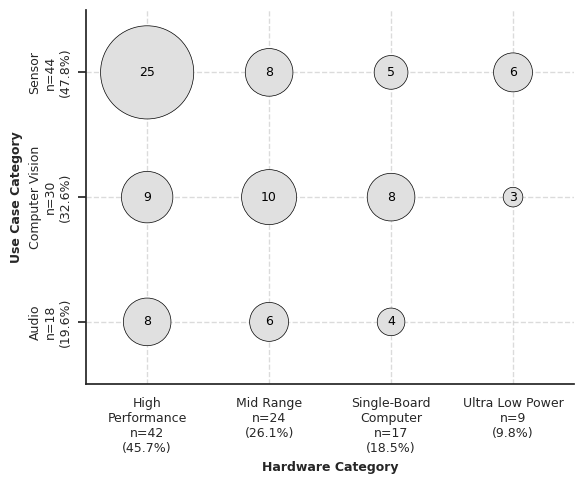
\includegraphics[width=0.8\textwidth]{figs/research_results/sms_hardware_use_case.png} 
    \caption[Mapping of Hardware Platforms to AI Use Cases]{Hardware platform distribution across AI use case categories.}
    \label{fig:bubble-chart-hardware-vs-aiusecase} % Umbenannt für Eindeutigkeit
\end{figure}

Figure~\ref{fig:bubble-chart-hardware-vs-aiusecase} illustrates the relationship between hardware platforms and \gls{ai} use cases. The visualization reveals distinct patterns providing insights into current \gls{tinyml} implementation priorities. For a granular breakdown of specific \gls{ai} applications, refer to Appendix~\ref{app:detailed-ai-use-cases} (Figure~\ref{fig:detailed-ai-use-cases}).

The most prominent pattern is the substantial concentration of High-Performance hardware implementations for Sensor-based applications ($n=25$). This represents the largest single category, suggesting sensor data processing—despite potential assumptions of lower computational needs—currently favors more capable hardware in practice. Examples include \cite{antoniniTinyMLOpsFrameworkOrchestrating2022} (industrial anomaly detection using high-performance \glspl{mcu}) and \cite{fraidlingTinyMachineLearning2023} (sensor data fusion on an STM32-F746NG platform). This may reflect requirements for real-time processing of multiple sensor streams, complex fusion algorithms, or accommodation of continuous on-device learning.

For Computer Vision use cases, closer examination reveals nuances. While Mid-Range hardware shows the highest frequency ($n=10$), these implementations often represent simpler binary classification tasks rather than complex object detection or segmentation. For more advanced computer vision, \glspl{sbc} demonstrate greater prevalence \cite{renOndeviceOnlineLearning2024}. High-Performance platforms ($n=9$) maintain substantial representation across vision tasks, while Ultra-Low-Power devices ($n=3$) show limited adoption, primarily for constrained classification scenarios. Audio processing exhibits a distinct hardware profile: High-Performance platforms ($n=8$) lead, followed by Mid-Range devices ($n=6$) and \glspl{sbc} ($n=4$). As shown in \cite{grauOnDeviceTrainingMachine2021}, keyword spotting is a common audio application on mid-range hardware (e.g., Arduino Nano 33 BLE, Cortex-M4 based platforms). The absence of Ultra-Low-Power devices in audio processing suggests technical barriers for audio-based \gls{tinymlops} on severely constrained hardware, likely due to continuous sampling and spectral processing demands.

\section{System Architectures in TinyML}
\label{sec:RQ1_Results_SystemArchitecture}

Analysis of the selected literature reveals a spectrum of recurring architectural patterns for integrating \gls{tinyml} systems with \gls{mlops} practices, as summarized in Table~\ref{tab:architectural_patterns_overview}. These patterns are not always mutually exclusive; many contemporary \gls{tinyml} systems exhibit hybrid characteristics, borrowing elements from multiple established approaches to achieve desired performance and functionality. Categorized by their primary locus of control and computation—ranging from centralized cloud-dependent models to fully decentralized edge-native solutions—this strategic balancing reflects a growing understanding of harnessing distributed resources effectively for specific application demands and hardware constraints. The subsequent discussion (Sections~\ref{ssec:centralized_hybrid_arch} and \ref{ssec:decentralized_edge_native_arch}) elaborates on these categories, linking them to research contributions and inherent trade-offs.

\begin{landscape}
    \begin{table}[htbp]
        \caption[Overview of System Architecture Patterns]{\emph{Synthesized Overview} of System Architecture Patterns in \gls{tinyml}/\gls{mlops}}
        \label{tab:architectural_patterns_overview}
        \scriptsize
        \renewcommand{\arraystretch}{1.2}
        \setlength{\tabcolsep}{4pt} % Unified tabcolsep
        \begin{tabularx}{\linewidth}{@{} >{\RaggedRight\bfseries\arraybackslash}X % First column now bold by spec
                                     >{\RaggedRight\arraybackslash}X
                                     >{\RaggedRight\arraybackslash}X
                                     >{\RaggedRight\arraybackslash}X
                                     >{\RaggedRight\arraybackslash}X
                                     >{\RaggedRight\arraybackslash}X @{}}
            \toprule
            \hl{\footnotesize\textbf{Architectural Pattern}} &
            \hl{\footnotesize\textbf{Key Components}} &
            \hl{\footnotesize\textbf{Dependencies}} &
            \hl{\footnotesize\textbf{Strengths}} &
            \hl{\footnotesize\textbf{Limitations}} &
            \hl{\footnotesize\textbf{Example (Papers)}} \\
            \midrule
            Data-Centric & 
                Data acquisition, preprocessing modules; Feature extraction, data storage (on-device/edge); Data buffers; on-device/edge learning mechanisms &
                Data availability \& quality; Local processing capacity; Efficient algorithms; Communication for data offloading &
                Optimized data handling; Supports continuous learning \& adaptation to local conditions/drift; Model robustness; Potential for personalization; Reduces data transmission overhead &
                Resource-intensive for complex on-device processing/feature extraction; Relies heavily on data quality at the source; Managing consistency \& quality across devices; Potential for catastrophic forgetting if not managed &
                \cite{banburyEdgeImpulseMLOps2023}, \cite{disabatoIncrementalOnDeviceTiny2020}, \cite{renOndeviceOnlineLearning2024}, \cite{sudharsanEdge2TrainFrameworkTrain2020}, \cite{moskalenkoResilienceawareMLOpsResourceconstrained2023}, \cite{pavanTyBoxAutomaticDesign2024}, \cite{grauOnDeviceTrainingMachine2021}, \cite{fraidlingTinyMachineLearning2023}, \cite{demaghSensOLMemoryEfficientOnline2024} \\
            \midrule
            Client-Server / Edge-Cloud &
                \gls{mcu}/\gls{sbc} as client/edge node; Gateway; Cloud/edge server backend/platform; \gls{ml} tasks split (e.g., inference on device, training in cloud) &
                Network connectivity (may be intermittent); Server availability; Security of data in transit \& at rest; Communication protocols (e.g., \gls{mqtt}, gls{coap}, HTTP, ESP-NOW, \gls{lwm2m}) &
                Powerful cloud/server resources for complex tasks; Simpler/lower-cost edge devices; Centralized management \& \gls{ota} updates; Global model improvements; Edge processing can offer lower latency &
                Dependence on network connectivity and latency; Bandwidth costs/consumption; Privacy concerns with raw data transmission; Complexity in managing distributed components &
                \cite{antoniniTinyMLOpsFrameworkOrchestrating2022}, \cite{fraidlingTinyMachineLearning2023}, \cite{alselekAgileAIFirmware2024}, \cite{alselekDynamicAIIoTEnabling2024}, \cite{rajEdgeMLOpsAutomation2021}, \cite{doyuTinyMLaaSEcosystemMachine2021}, \cite{peltonenLinkEdgeOpensourcedMLOps2023}, \cite{sudharsanOTATinyMLAirDeployment2022}, \cite{zaidiUnlockingEdgeIntelligence2022}, \cite{condeEnhancedFIWAREBasedArchitecture2024}, \cite{huangRIOTMLToolkitOvertheair2024a} \\
            \midrule
            Component-Based &
                Modular software/hardware units (sensing, preprocessing, inference, communication, update agent, etc.) on device and/or server; optional cloud layer &
                Well-defined interfaces; Interface \& version compatibility; Orchestration mechanism &
                Modularity promotes reusability, maintainability, \& independent updates; Simplifies development \& maintenance; agile deployment \& easier replacement of parts &
                Integration complexity between components; Potential overhead from inter-component communication; Requires careful interface design; Resource partitioning challenges &
                \cite{szydloManagementTinyMLEnabled2024}, \cite{sudharsanEdge2TrainFrameworkTrain2020}, \cite{minSensiXBringingMLOps2023}, \cite{pavanTyBoxAutomaticDesign2024}, \cite{lootusVMContainerizedApproach2022}, \cite{fraidlingTinyMachineLearning2023}, \cite{condeEnhancedFIWAREBasedArchitecture2024}, \cite{antoniniTinyMLOpsFrameworkOrchestrating2022}, \cite{rajEdgeMLOpsAutomation2021} \\
            \midrule
            Microservices/\gls{soa} &
                Fine-grained, independent, loosely coupled, deployable services (model serving, data transformation, inference, etc.); APIs for inter-service communication (e.g., \gls{rest} APIs, message queues); Containerized \& managed by orchestrator &
                Network infrastructure; Inter-service communication; Service orchestration; API management, service discovery &
                High scalability \& flexibility; Fault isolation \& resilience; Heterogeneous components/frameworks; Independent development/deployment of services &
                Overhead (memory, compute, network, containerization) for resource-constrained devices; Increased complexity in deployment, management, \& orchestration; Higher latency/network overhead from inter-service calls &
                \cite{minSensiXBringingMLOps2023}, \cite{rajEdgeMLOpsAutomation2021}, \cite{condeEnhancedFIWAREBasedArchitecture2024}, \cite{lootusVMContainerizedApproach2022}, \cite{alselekAgileAIFirmware2024}       \\
            \midrule
            Distributed (Federated/Cooperative) &
                Multiple edge devices capable of local training; Optional central aggregation server (for \gls{fl}) or P2P links; Distributed training/\gls{fl} algorithms (e.g., FedAvg); Communication protocols for model updates/parameters &
                Network connectivity; Standardized model/update formats; Algorithms for model aggregation/consensus; Client participation; Handling stragglers \& data heterogeneity &
                Enhanced privacy (raw data stays local); Leverages knowledge from distributed datasets; Enables collaborative learning; Reduced communication bandwidth (only model updates/parameters shared); Improve model generalization \& robustness &
                Communication overhead for model updates; Complexity of distributed training, orchestration, synchronization; Managing stragglers \& device heterogeneity; Statistical heterogeneity can impede convergence; Security of aggregation process &
                \cite{gulatiTDMiLTinyDistributed2024}, \cite{renOndeviceOnlineLearning2024}, \cite{grauOnDeviceTrainingMachine2021}, \cite{alselekDynamicAIIoTEnabling2024} \\
            \bottomrule
        \end{tabularx}
    \end{table}
\end{landscape}

\subsection{Centralized and Hybrid Architectural Models}
\label{ssec:centralized_hybrid_arch}

A significant portion of \gls{tinyml} systems leverages centralized or hybrid architectural models, where a substantial part of the computational load, control logic, or complex model training resides in a more powerful backend, such as a cloud platform or an edge server. The classic \textit{Client-Server architecture} (often termed \textit{Edge-Cloud} in this context) is a prime example \cite{doyuTinyMLaaSEcosystemMachine2021, zaidiUnlockingEdgeIntelligence2022, peltonenLinkEdgeOpensourcedMLOps2023}. In this setup, resource-constrained \gls{tinyml} devices (clients) primarily handle data acquisition, local preprocessing, and optimized model inference. More demanding tasks—such as initial model training, extensive data processing, complex retraining, model optimization, and overarching \gls{mlops} orchestration including \gls{ci}/\gls{cd} pipelines—are offloaded to the server or cloud components. This division allows \gls{tinyml} devices to overcome their inherent resource limitations by leveraging scalable, centralized resources for storage and computation. Frameworks such as Edge Impulse \cite{banburyEdgeImpulseMLOps2023}, and platforms like Azure IoT Edge, AWS IoT Greengrass, and LinkEdge \cite{peltonenLinkEdgeOpensourcedMLOps2023}, embody this hybrid pattern, often utilizing containerization concepts for deploying and managing \gls{ml} models. The strength of such architectures lies in centralized control, enabling streamlined remote model updates (\gls{ota}), comprehensive monitoring, and adaptation of models. The Edge \gls{mlops} framework by Raj et al.~\cite{rajEdgeMLOpsAutomation2021} further exemplifies this by demonstrating a \gls{ci}/\gls{cd} pipeline that deploys containerized models from a cloud orchestrator to edge devices.

\textit{Component-Based architectures} and \textit{Microservice/\gls{soa} architectures} also frequently manifest within this centralized or hybrid paradigm, particularly when a central orchestrator or cloud backend manages the deployment and interaction of modular components or fine-grained services. For instance, SensiX++ \cite{minSensiXBringingMLOps2023} employs modular components for data coordination and model serving on the edge device, but these are typically part of a larger system where model updates and high-level orchestration are managed centrally. Similarly, microservices deployed on edge gateways might interact with cloud-based services for advanced analytics or model retraining. Components like data coordinators, model servers, and adaptive schedulers often interact within the server/cloud layer to manage the lifecycle of \gls{ml} models destined for the edge. While full microservice deployments are less common directly on severely constrained \glspl{mcu} due to overhead, the principles of modularity and isolated execution are explored, as seen with concepts like ``Runes'' aiming for container-like packages on \glspl{mcu} \cite{lootusVMContainerizedApproach2022}. The emergence of ``as-a-Service'' models, such as \gls{tmlaas} \cite{doyuTinyMLaaSEcosystemMachine2021}, explicitly embodies this hybrid approach, offering \gls{ml} capabilities to constrained devices through services hosted at the edge or in the cloud. The primary advantages include leveraging powerful centralized resources and maintaining a unified control plane. However, these models inherently depend on reliable network connectivity, and data transmission can introduce latency and raise privacy concerns, although edge processing can mitigate some risks.

\subsection{Decentralized and Edge-Native Architectural Models}
\label{ssec:decentralized_edge_native_arch}

In contrast to centralized models, a growing body of research explores decentralized and edge-native architectures that prioritize local processing, device autonomy, and reduced reliance on continuous cloud connectivity. \textit{Data-Centric architectures} represent a key trend, emphasizing the processing of data as close to its source as possible. Instead of primarily streaming raw data, these systems perform significant data analysis, feature extraction, and often model inference directly on the device, conserving energy and bandwidth \cite{fraidlingTinyMachineLearning2023, antoniniTinyMLOpsFrameworkOrchestrating2022}.

\textit{Distributed architectures}, particularly those employing \gls{fl}, further advance decentralization \cite{gulatiTDMiLTinyDistributed2024, grauOnDeviceTrainingMachine2021}. In \gls{fl}, models are trained collaboratively across multiple edge devices using their respective local data. Only model updates (e.g., parameters or gradients) are shared and aggregated (centrally or peer-to-peer) to create an improved global model, without exposing raw local data. This enhances data privacy, reduces communication bandwidth, and can lower inference latency. Frameworks like TDMiL \cite{gulatiTDMiLTinyDistributed2024}, and research into TinyFL, TinyReptile, and TinyMetaFed \cite{renOndeviceOnlineLearning2024} explore strategies for implementing such distributed learning on resource-constrained \glspl{mcu}.

Beyond collaborative training, on-device learning capabilities allow individual \gls{tinyml} devices to update or fine-tune their models locally using new data encountered in the field \cite{disabatoIncrementalOnDeviceTiny2020, renOndeviceOnlineLearning2024}. This addresses performance degradation due to concept drift. Approaches like TinyOL \cite{renOndeviceOnlineLearning2024}, Train++ \cite{sudharsanEdge2TrainFrameworkTrain2020}, and incremental \gls{knn} classifiers \cite{disabatoIncrementalOnDeviceTiny2020} enable learning or adaptation directly on \glspl{mcu}, though this faces challenges due to limited memory for training data and computational constraints for algorithms like backpropagation.

\textit{Component-Based} and \textit{Microservice/\gls{soa}} designs can also be implemented in a fully edge-native manner, focusing on on-device modularity and inter-component communication without strong dependency on a central server for core operations. Lootus et al.'s ``Runes'' concept \cite{lootusVMContainerizedApproach2022}, for instance, aims to provide portable, container-like execution environments for \gls{tinyml} applications directly on diverse \glspl{mcu}. The main strengths of these decentralized models are enhanced device autonomy, improved data privacy, and reduced operational latency. However, they place greater demands on the limited resources of edge devices and can introduce complexities in coordinating distributed components and managing system-wide consistency.


\section{Frameworks and Tools for On-Device MLOps}
\label{sec:RQ2_Results_Frameworks}

This section analyzes relevant frameworks, and strategies for continuous \gls{lcm}. Specifically, the discussion will cover identified frameworks enabling such decentralized operations (Section~\ref{ssec:identified_frameworks_rq2}), commonly utilized standard tools and libraries (Section~\ref{ssec:standard_tools_libraries_rq2}), and a synthesis of core contributions and overarching strategies (Section~\ref{ssec:core_contributions_strategies_rq2}).

\subsection{Identified Frameworks for Decentralized On-Device MLOps}
\label{ssec:identified_frameworks_rq2}

The systematic review of the selected literature reveals several frameworks explicitly designed or adapted to support decentralized on-device \gls{mlops}. To provide a concise overview, these frameworks can be clustered by their primary purpose and contribution towards enabling on-device intelligence and reducing cloud dependency. Table~\ref{tab:frameworks_ondevice_mlops_clustered} presents this categorized summary, listing the frameworks within each category, their collective key on-device \gls{mlops} features, and common strategies for minimizing cloud reliance.

\begin{landscape}
\begin{table}[htbp]
    \caption{Clustered Overview of Frameworks for Decentralized On-Device \gls{mlops}}
    \label{tab:frameworks_ondevice_mlops_clustered}
    \scriptsize % Base font size for the table content
    \renewcommand{\arraystretch}{1.2}
    \setlength{\tabcolsep}{4pt}
    \begin{tabularx}{\linewidth}{%
        >{\RaggedRight\bfseries}X% Framework Category/Purpose
        >{\RaggedRight\arraybackslash}X% Frameworks (Name [Source])
        >{\RaggedRight\arraybackslash}X% Key On-Device MLOps Features
        >{\RaggedRight\arraybackslash}X% Strategy for Minimizing Cloud Reliance
    }
    \toprule 
    \multicolumn{1}{>{\RaggedRight}X}{\hl{\footnotesize\textbf{Framework Category / Purpose}}} & 
    \multicolumn{1}{>{\RaggedRight}X}{\hl{\footnotesize\textbf{Frameworks (Name [Source])}}} & 
    \multicolumn{1}{>{\RaggedRight}X}{\hl{\footnotesize\textbf{Key On-Device \gls{mlops} Features}}} & 
    \multicolumn{1}{>{\RaggedRight}X}{\hl{\footnotesize\textbf{Strategy for Minimizing Cloud Reliance}}} \\ 
    \midrule 

    On-Device Learning \& Adaptation &
        % Using a compact itemize list
        \begin{itemize}[nosep,leftmargin=*,after=\strut]
            \item Train++ \cite{sudharsanTrainIncrementalML2021}
            \item Edge2Train \cite{sudharsanEdge2TrainFrameworkTrain2020}
            \item TinyOL \cite{renOndeviceOnlineLearning2024}
            \item TyBox \cite{pavanTyBoxAutomaticDesign2024}
            \item LifeLearner \cite{kwonLifeLearnerHardwareAwareMeta2023}
            \item SensOL \cite{demaghSensOLMemoryEfficientOnline2024}
            \item TML-CD \cite{disabatoTinyMachineLearning2024}
        \end{itemize} &
        Incremental/online learning algorithms; on-device classifier/model modification and (re)training; local data processing for adaptation; handling of concept drift; memory-efficient replay/storage for continual learning. &
        Localizes model training, fine-tuning, and adaptation on-device using live/streaming data, significantly reducing or eliminating the need for cloud-based retraining services and continuous data transfer. Enables self-learning and autonomous device behavior. \\
    \addlinespace

    Federated \& Distributed Learning &
        \begin{itemize}[nosep,leftmargin=*,after=\strut]
            \item TinyReptile \cite{renOndeviceOnlineLearning2024}
            \item TinyMetaFed \cite{renOndeviceOnlineLearning2024}
            \item TDMiL \cite{gulatiTDMiLTinyDistributed2024}
            \item On-Device Training (Grau) \cite{grauOnDeviceTrainingMachine2021}
        \end{itemize} &
        Collaborative model training across multiple devices; aggregation of model updates (e.g., parameters, gradients) locally or via a lightweight coordinator; on-device learning steps (e.g., \gls{sgd}); optimized communication protocols for constrained networks. &
        Enables knowledge sharing and global model improvement from distributed data sources without centralizing raw data, enhancing privacy. Reduces reliance on powerful central cloud servers for training entire models from scratch. \\
    \addlinespace

    Model Deployment \& \gls{ota} Updates &
        \begin{itemize}[nosep,leftmargin=*,after=\strut]
            \item Dynamic AI-IoT \cite{alselekDynamicAIIoTEnabling2024}
            \item OTA-TinyML \cite{sudharsanOTATinyMLAirDeployment2022}
            \item DevOps-based \gls{mlops} \cite{alselekAgileAIFirmware2024}
        \end{itemize} &
        Secure Over-The-Air (\gls{ota}) updates for firmware, \gls{ml} models (full or partial); dynamic loading and switching of models on-device without full firmware reflashing; \gls{ci}/\gls{cd} pipelines tailored for low-power devices. &
        Facilitates remote and efficient management of device software and \gls{ml} models, minimizing physical interventions and reducing bandwidth/complexity associated with cloud-managed fleet updates. \\
    \addlinespace

    Comprehensive \gls{mlops} Platforms \& Toolkits &
        \begin{itemize}[nosep,leftmargin=*,after=\strut]
            \item Edge Impulse \cite{banburyEdgeImpulseMLOps2023}
            \item RIOT-ML \cite{huangRIOTMLToolkitOvertheair2024a}
            \item Edge MLOps \cite{rajEdgeMLOpsAutomation2021}
            \item FIWARE-based Arch. \cite{alselekAgileAIFirmware2024} % Assuming this is the correct citation for the FIWARE arch. mentioned earlier
            \item LinkEdge \cite{peltonenLinkEdgeOpensourcedMLOps2023}
            \item Tiny-MLOps \cite{antoniniTinyMLOpsFrameworkOrchestrating2022}
        \end{itemize} &
        End-to-end workflow support (data acquisition to deployment); on-device performance estimation, monitoring, and evaluation; model optimization for edge hardware; automated deployment mechanisms; integration with \gls{iot} platforms and \gls{ci}/\gls{cd} tools. &
        Streamlines the entire \gls{mlops} lifecycle for edge/\gls{tinyml} devices. Often employs a hybrid cloud-edge model but delegates significant operational autonomy, model execution, and management tasks to the edge, reducing constant cloud interaction. \\
    \addlinespace

    Specialized \gls{mlops} Aspects &
        \begin{itemize}[nosep,leftmargin=*,after=\strut]
            \item SensiX++ \cite{minSensiXBringingMLOps2023} (Model Serving)
            \item Resilience-aware \gls{mlops} \cite{moskalenkoResilienceawareMLOpsResourceconstrained2023} (Resilience)
            \item SeLoC-ML \cite{renOndeviceOnlineLearning2024}
             (Resource Management)
        \end{itemize} &
        Optimized on-device model serving and inference; adaptive scheduling; post-hoc resilience optimization (e.g., uncertainty calibration, test-time adaptation); semantic management of \gls{tinyml} resources (models, devices) at scale. &
        Enhances specific operational qualities like inference efficiency, model robustness against disturbances, and large-scale manageability directly on or for edge devices, thereby reducing the need for cloud intervention for these specialized tasks. \\
    \addlinespace

    Deployment \& Abstraction Services (SaaS-like) &
        \begin{itemize}[nosep,leftmargin=*,after=\strut]
            \item TinyMLaaS Ecosystem \cite{doyuTinyMLaaSEcosystemMachine2021, zaidiUnlockingEdgeIntelligence2022}
        \end{itemize} &
        Hardware/software agnostic \gls{ml} model deployment; compiler plugin interfaces for diverse targets; orchestration protocols (e.g., \gls{lwm2m}); standardized inference module formats. &
        Simplifies and democratizes \gls{tinyml} deployment by providing standardized services, potentially edge-hosted, that abstract underlying complexities. Reduces direct device-to-cloud interaction for model compilation and deployment tasks. \\
    \bottomrule
    \end{tabularx}
\end{table}
\end{landscape}

\subsection{Commonly Utilized Standard Tools and Libraries}
\label{ssec:standard_tools_libraries_rq2}

Beyond the specific frameworks proposed in primary studies, a wide array of standard tools and libraries are frequently referenced and utilized to construct and support \gls{tinymlops} workflows. These tools often serve as building blocks within more comprehensive frameworks or are used independently to address specific phases of the \gls{ml} lifecycle. Table~\ref{tab:standard_tools_libraries_mlops} categorizes these commonly mentioned tools and libraries by their relevant \gls{mlops} phase.

\begin{longtable}{>{\RaggedRight\arraybackslash}p{0.25\linewidth} >{\RaggedRight\arraybackslash}p{0.7\linewidth}}
\caption[Standard Tools and Libraries in TinyMLOps]{Standard Tools and Libraries Mentioned in Literature for Various \gls{tinymlops} Phases} \label{tab:standard_tools_libraries_mlops} \\
\toprule
\textbf{MLOps Phase(s)} & \textbf{Standard Tools/Libraries Mentioned} \\
\midrule
\endfirsthead
\multicolumn{2}{c}%
{{\bfseries Table \thetable\ continued from previous page}} \\
\toprule
\textbf{MLOps Phase(s)} & \textbf{Standard Tools/Libraries Mentioned} \\
\midrule
\endhead
\midrule
\multicolumn{2}{r}{{Continued on next page}} \\
\endfoot
\bottomrule
\endlastfoot

General Platform/OS & MicroPython (Optimized Python for \glspl{mcu}), RIOT (Low-power \gls{iot} OS), Zephyr (RTOS), Embedded Linux, RaspbianOS \\
\addlinespace
Data Collection & \gls{iot} Agents (FIWARE), \gls{mqtt} (Messaging protocol), Mosquitto (\gls{mqtt} broker), DVC (Data Version Control), Label Studio (Labeling) \\
\addlinespace
Data Processing/Preparation & DSP Pipeline (Edge Impulse), FIWARE Draco (Apache NiFi), ulab (NumPy-like for MP), tsfresh/sktime (Feature extraction) \\
\addlinespace
Training & TensorFlow, Keras, Scikit-learn, PyTorch, Pure Python or C++ \\
\addlinespace
Evaluation & MLPerf Tiny (Benchmark suite), U-TOE (On-board evaluation) \\
\addlinespace
Optimization/Conversion & \gls{tfl}, \gls{tfl} \gls{tflm}, STM32Cube.AI, \gls{onnx}, TVM/uTVM (Compiler), Emlearn (\gls{ml} to C) \\
\addlinespace
Deployment/Update & GitLab \gls{ci}/\gls{cd}, Docker/Docker Compose, Kubernetes, Helm, \gls{lwm2m}, \gls{coap}, \gls{dtls}, \gls{ota} \\
\addlinespace
Monitoring/Analytics & Grafana (Dashboard), InfluxDB (Time series DB), MLflow/Neptune (\gls{ml} tracking), Edge Fleet Analytics (Edge \gls{mlops}) \\
\addlinespace
Management/Orchestration & FIWARE (\gls{iot} platform), Context Broker (FIWARE), \gls{ngsi}, Apache Airflow \\
\end{longtable}

\subsection{Core Contributions and Strategies for Decentralized MLOps}
\label{ssec:core_contributions_strategies_rq2}

The identified frameworks and tools contribute to decentralized on-device \gls{mlops} through several core strategies. These strategies collectively aim to enhance the autonomy of \gls{tinyml} devices, reduce their reliance on cloud infrastructure, and address the unique challenges of managing \gls{ml} lifecycles in resource-constrained environments.

\paragraph{End-to-End Platforms and Orchestration Frameworks}
Several proposed solutions focus on providing comprehensive, often end-to-end platforms or robust orchestration capabilities for \gls{tinymlops}. These systems streamline the \gls{ml} lifecycle by coordinating activities across heterogeneous devices. Platforms like Edge Impulse, while cloud-assisted for development, generate highly optimized on-device inference libraries, significantly reducing the device's need for cloud interaction during operation \cite{banburyEdgeImpulseMLOps2023}. The Tiny-MLOps framework adapts standard \gls{mlops} practices for far-edge \glspl{mcu}, enabling them to be active computational elements in the \gls{ml} loop \cite{antoniniTinyMLOpsFrameworkOrchestrating2022}. SensiX++ facilitates multi-tenant model serving on sensory edge devices \cite{minSensiXBringingMLOps2023}, while LinkEdge \cite{peltonenLinkEdgeOpensourcedMLOps2023} and Edge \gls{mlops} \cite{rajEdgeMLOpsAutomation2021} provide pipelines for automating deployment and management closer to the edge, with Edge \gls{mlops} employing a hybrid cloud-edge model that triggers edge-level actions based on local monitoring. FIWARE-based architectures integrate \gls{tinyml} into broader cyber-physical system management \cite{alselekAgileAIFirmware2024}. Toolkits like RIOT-ML offer integrated solutions for \gls{ci}/\gls{cd} and \gls{ota} updates on low-power \gls{iot} devices \cite{huangRIOTMLToolkitOvertheair2024a}. The SeLoC-ML framework uses Semantic Web technologies for scalable management of diverse \gls{tinyml} resources, simplifying deployment and enhancing interoperability \cite{renOndeviceOnlineLearning2024}. These platforms often provide structured workflows that automate various \gls{mlops} stages, pushing capabilities towards the edge.

\paragraph{Enabling On-Device Intelligence: Learning, Adaptation, and Optimization}
A critical aspect of minimizing cloud reliance is empowering \gls{tinyml} models to learn, adapt, or optimize locally. Frameworks like Edge2Train \cite{sudharsanEdge2TrainFrameworkTrain2020}, Train++ \cite{sudharsanTrainIncrementalML2021}, TinyOL \cite{renOndeviceOnlineLearning2024}, SensOL \cite{demaghSensOLMemoryEfficientOnline2024}, and TyBox \cite{pavanTyBoxAutomaticDesign2024} introduce algorithms and libraries for direct on-\gls{mcu} training or incremental learning, enabling adaptation to concept drift without continuous cloud intervention. The TML-CD \cite{disabatoTinyMachineLearning2024} solution specifically focuses on on-device adaptation to concept drift. Distributed on-device learning is advanced by frameworks like TDMiL, TinyReptile, and TinyMetaFed, which facilitate \gls{fl} or meta-learning across multiple devices, sharing only model updates or aggregated knowledge, thus preserving data privacy and reducing communication overhead \cite{gulatiTDMiLTinyDistributed2024}. LifeLearner employs hardware-aware meta-continual learning for efficient adaptation on constrained devices \cite{kwonLifeLearnerHardwareAwareMeta2023}. Furthermore, optimization tools such as \gls{tflm}, STM32Cube.AI, and uTVM are crucial for converting and optimizing models (e.g., through quantization and pruning) for efficient execution within the tight resource budgets of \glspl{mcu} \cite{davidTensorFlowLiteMicro2021}. This local processing and adaptation capability is foundational to creating \gls{tinyml} systems.

\paragraph{Deployment, Operational Management, and System Resilience}
Effective deployment, management, and ensuring the robustness of \gls{tinyml} models on numerous decentralized devices are key operational challenges. \gls{ota} updating is a cornerstone for managing remote devices, with frameworks like OTA-TinyML \cite{sudharsanOTATinyMLAirDeployment2022} and toolkits such as RIOT-ML \cite{huangRIOTMLToolkitOvertheair2024a} providing mechanisms for efficient and secure remote deployment of models and firmware, often using lightweight protocols like \gls{lwm2m} and \gls{coap}. Containerization concepts, explored by efforts like the Rune framework, aim to standardize application packaging for diverse hardware \cite{lootusVMContainerizedApproach2022}. For operational management at scale, semantic frameworks like SeLoC-ML offer unified administration of models and devices \cite{renOndeviceOnlineLearning2024}. The \gls{tmlaas} concept envisions an ecosystem to abstract hardware and software complexities, simplifying model deployment \cite{doyuTinyMLaaSEcosystemMachine2021}. System resilience is addressed by frameworks like ``Resilience-aware \gls{mlops}'', which incorporate stages for optimizing robustness against disturbances  through techniques like uncertainty quantification and test-time adaptation on the device itself \cite{moskalenkoResilienceawareMLOpsResourceconstrained2023}. These contributions are vital for maintaining reliable \gls{tinyml} systems with minimal cloud dependency for operational tasks.

\section{Concluding Synthesis of Research Findings}
\label{sec:Concluding_Synthesis_Research_Results}

The findings from this systematic review reveal that current \gls{tinymlops} research is predominantly characterized by the proposal of foundational frameworks, which, while innovative, often await rigorous empirical validation. Dominant trends include a focus on more capable \glspl{mcu} for sensor-based analysis, computer vision, and audio processing. Architecturally, Data-Centric and Client-Server patterns prevail, typically employing Centralized Training and Offline Learning with static, pre-trained models. These approaches commonly integrate established \gls{mlops} practices like model versioning and optimization techniques such as quantization and purning.

Despite the prevalence of centralized methods, a clear and significant trend towards greater on-device intelligence and operational autonomy exists. Substantial research investigates decentralized and hybrid training models that foster on-device learning—be it incremental or online—and adaptation to phenomena like concept drift. An increasing number of specialized frameworks and tools focused on local processing, efficient \gls{ota} updates, and comprehensive edge-native \gls{mlops} strategies. The core motivations remain consistent: reducing latency, enhancing data privacy, and ensuring robust operation with minimized reliance on continuous cloud connectivity.

Several challenges and opportunities for advancement persist within the field. There is a clear need for more widespread adoption of comprehensive \gls{lcm} practices, particularly for adaptive systems. While basic monitoring of model accuracy and latency is common, more sophisticated and resource-aware monitoring for dynamic on-device environments, including robust drift detection, requires further attention. Furthermore, the practical application of advanced optimization techniques specifically for on-device learning scenarios, alongside the maturation of standardized toolchains and interfaces, remains an active area of development.
%!TEX root = thesis.tex

\chapter{Conceptual Design of a TinyMLOps Ecosystem}
\label{chp:Framework}

Building upon the systematic literature review in Chapter~\ref{chp:Research_Results}, which identified critical gaps in operationalizing \gls{ml} on resource-constrained edge devices, this chapter introduces the conceptual design of a novel, integrated ecosystem for autonomous \gls{tinymlops}. This ecosystem is architected to address the challenges of managing the \gls{ml} model lifecycle directly on edge hardware with minimal reliance on centralized infrastructure, while also providing pathways for optional, synergistic server-side support. The ecosystem comprises two primary components: (i) \gls{tinylcm}, an on-device framework engineered for autonomous \gls{ml} model execution, monitoring, and adaptation; and (ii) TinySphere, a server-side platform designed to provide enhanced \gls{mlops} capabilities, including model validation, fleet management, and advanced analytics, specifically tailored to the nuances of \gls{tinyml} deployments.

~\\
\vfill
\minitoc
\clearpage

\section{Motivation and Design Rationale}
\label{sec:framework_motivation_rationale}

Deploying and sustainably operating \gls{ml} models on severely resource-constrained edge devices, such as \gls{mcu} and low-power \gls{sbc}, presents distinct challenges. Traditional \gls{mlops} paradigms, primarily designed for cloud environments with abundant resources, do not adequately address these specific edge-related issues \cite{lerouxTinyMLOpsOperationalChallenges2022a, szydloManagementTinyMLEnabled2024}.

\subsection{Revisiting Research Gaps and Limitations}
\label{ssec:framework_revisiting_gaps}

The findings from Chapter~\ref{chp:Research_Results} (particularly Sections~\ref{sec:RQ1_Results_SystemArchitecture} and \ref{sec:RQ2_Results_Frameworks}) indicate a rapidly evolving yet fragmented \gls{tinyml} operations landscape. Despite significant progress in model compression, on-device inference optimization, and specialized hardware, a cohesive, end-to-end framework for \textit{autonomous} on-device \gls{lcm} is still a critical unmet need.

Many contemporary approaches, even those targeting edge deployment, rely considerably on cloud infrastructure for \gls{mlops} tasks such as continuous model monitoring, retraining, and deploying updated models \cite{kreuzbergerMachineLearningOperations2023, antoniniTinyMLOpsFrameworkOrchestrating2022}. This dependency curtails the operational autonomy of edge devices. Consequently, it poses significant limitations for applications in environments with intermittent, unreliable, or non-existent connectivity—a common characteristic in numerous \gls{tinyml} use cases, such as the Mars rover scenario motivating this thesis.

Furthermore, existing platforms, while powerful within their specific domains, often do not meet the holistic requirements for managing adaptive, autonomous fleets of devices. For instance, platforms such as Edge Impulse provide robust support for the initial development, optimization, and deployment pipeline of \gls{tinyml} models \cite{banburyEdgeImpulseMLOps2023}. However, their primary focus is less on continuous, autonomous on-device adaptation of deployed models or the operational management of numerous, independently evolving devices.

Similarly, generic \gls{mlops} tools like MLflow offer strong capabilities for experiment tracking, model versioning, and deployment in server-based settings \cite{johnMLOpsFrameworkMaturity2021}. Yet, they are not inherently designed for the specific nuances of the \gls{tinyml} context. These nuances include extreme resource constraints (memory, power, computation), the imperative for on-device intelligence, and the need for resilient interaction with device-specific lifecycle processes.

The literature analysis (Chapter~\ref{chp:Research_Results}) also revealed that the integration of comprehensive device management within dedicated \gls{tinymlops} frameworks is still at a nascent stage; this feature, noted as beneficial in systems like SensiX++ \cite{minSensiXBringingMLOps2023}, is not yet widely incorporated. This confluence of observations underscores a pressing need: a server-side \gls{mlops} platform purposefully architected for the \gls{tinyml} paradigm. Such a platform must understand, interact with, and augment autonomous on-device operations, rather than merely adapting existing cloud-centric tools.

\subsection{Objectives and Core Tenets for the Ecosystem}
\label{ssec:framework_derived_objectives}

The aforementioned research gaps and limitations directly inform the primary objectives and guiding architectural principles for the proposed \gls{tinymlops} ecosystem. The overarching goal is to empower resource-constrained edge devices with genuine operational autonomy throughout the entire \gls{ml} model lifecycle. This entails enabling devices to independently monitor their operational context, detect and adapt to changes such as concept drift, manage their own state, and continue functioning effectively even without external communication. Concurrently, the ecosystem provides an optional, yet deeply synergistic, server-side infrastructure (TinySphere) for enhanced management, centralized validation, fleet oversight, and advanced analytics when connectivity and resources permit. This dual-component architecture aims for a pragmatic balance between maximal on-device self-sufficiency and the recognized benefits of centralized \gls{mlops} capabilities.

The ecosystem's design philosophy is ``autonomy-first.'' The on-device framework, \gls{tinylcm}, is engineered as the primary locus of intelligence, performing all critical lifecycle functions locally. These include continuous, label-agnostic monitoring for concept drift, on-device model adaptation in response to detected changes, and robust local state management, including versioning and rollback facilities. The server-side platform, TinySphere, is conceived as an optional, value-adding component, designed to ingest operational data and events from \gls{tinylcm} instances. It offers advanced analytical capabilities, facilitates external validation of on-device adaptations, and provides comprehensive fleet management functionalities.

In terms of architectural patterns, informed by the findings in Chapter~\ref{chp:Research_Results} (Section~\ref{sec:RQ1_Results_SystemArchitecture}), the proposed ecosystem strategically combines established paradigms. For the on-device \gls{tinylcm} framework, a \textit{data-centric pipeline architecture} is adopted. This choice is motivated by its prevalence in existing \gls{tinyml} systems (as identified in Section~\ref{ssec:SystemArchitectureResults}) and its inherent suitability for efficiently processing sequential data streams on edge devices, facilitating modularity and a clear flow of operations from feature extraction through drift detection and adaptation. For the interaction between \gls{tinylcm} and TinySphere, an \textit{client-server model} is employed. While a client-server dependency might seem to contradict the autonomy goal, this pattern is implemented such that \gls{tinylcm} functions independently, attempting to engage with TinySphere only when network connectivity is available and interaction is beneficial (e.g., for data offloading or validation). This server-side interaction is considered crucial for realizing a full spectrum of \gls{mlops} capabilities. The design of TinySphere itself directly responds to the lack (identified in Section~\ref{ssec:framework_revisiting_gaps}) of TinyML-centric \gls{mlops} platforms supporting such a hybrid autonomous-collaborative operational model.

\section{System Requirements and Architectural Vision}
\label{sec:framework_requirements_vision}

To translate the objectives and design rationale into a concrete system, this section establishes functional and non-functional requirements. These requirements are directly informed by the preceding literature analysis (Chapter~\ref{chp:Research_Results}), the overarching goal of enabling autonomous on-device \gls{ml} \gls{lcm}, and the operational challenges exemplified by the Mars rover case study which serves as a guiding scenario. Subsequently, a high-level architectural vision for the complete ecosystem, illustrating the interplay between its on-device and server-side components, is presented.

\subsection{Functional and Non-Functional Requirements}
\label{ssec:framework_requirements}

The functional requirements (FR) define the core capabilities that the ecosystem must deliver to achieve its objectives. The non-functional requirements (NFR) specify the essential quality attributes that govern its performance, usability, and suitability for operation in resource-constrained environments. These are summarized in Table~\ref{tab:functional_requirements} and Table~\ref{tab:non_functional_requirements_v2}.

\begin{table}[htbp]
    \caption[Functional Requirements for the TinyMLOps Ecosystem]{Functional Requirements for the TinyMLOps Ecosystem.}
    \label{tab:functional_requirements}
    \begin{tabularx}{\linewidth}{@{}lX@{}}
        \opentableheader
        \hl{ID} & \hl{Description} \\
        \closetableheader
        FR1 & \textit{Autonomous On-Device Drift Detection:} The on-device component must be capable of continuously monitoring input data characteristics and/or model behavior to detect potential concept drift using proxy metrics, without requiring real-time ground truth labels. \\
        FR2 & \textit{Informed On-Device Model Adaptation:} Upon detection of a potential drift, \gls{tinylcm} must provide mechanisms for immediate, yet cautious, on-device adaptation of the deployed \gls{ml} model. \\
        FR3 & \textit{Robust On-Device State Management:} \gls{tinylcm} must implement robust state management, including versioning of models and relevant operational states, to enable rollbacks to previous stable states if an adaptation proves detrimental or an error occurs. \\
        FR4 & \textit{Opportunistic Synchronization:} \gls{tinylcm} must support optional and opportunistic synchronization of its state, operational logs, detected drift events, and (pseudo-)labeled data with a designated server-side component. \\
        FR5 & \textit{Centralized Monitoring and Fleet Management:} TinySphere should provide capabilities for the centralized monitoring of a fleet of deployed devices, offering insights into their operational status, model performance, and encountered drift phenomena. \\
        FR6 & \textit{Flexible Operational Modes:} The ecosystem must support distinct operational modes, ranging from purely autonomous on-device operation to fully server-assisted adaptive learning, configurable per device or application. \\
        \bottomrule
    \end{tabularx}
\end{table}

\begin{table}[htbp]
    \caption[Non-Functional Requirements for the TinyMLOps Ecosystem]{Non-Functional Requirements for the TinyMLOps Ecosystem.}
    \label{tab:non_functional_requirements_v2}
    \begin{tabularx}{\linewidth}{@{}lX@{}}
        \opentableheader
        \hl{ID} & \hl{Description} \\
        \closetableheader
        NFR1 & \textit{Resource Efficiency:} All on-device components must be optimized for minimal consumption of memory (RAM and flash), CPU cycles, and power, suitable for deployment on \glspl{mcu} and low-power \glspl{sbc}. \\ % Changed to \glspl
        NFR2 & \textit{Modularity and Extensibility:} Both \gls{tinylcm} and TinySphere must be designed with a modular architecture, allowing for straightforward extension or replacement of individual components (e.g., drift detection algorithms, classifiers, server-side analysis modules). \\
        NFR3 & \textit{Scalability:} The server-side platform must be designed to handle data and communication from a potentially large number of connected edge devices. \\
        NFR4 & \textit{Reliability and Fault Tolerance:} The on-device framework must operate reliably under adverse conditions, and synchronization mechanisms must be fault-tolerant, capable of resuming after interruptions. \\
        NFR5 & \textit{Configurability:} Key parameters of \gls{tinylcm}, such as drift detection sensitivity, adaptation strategies, and synchronization policies, must be configurable to suit diverse application needs and hardware capabilities. \\
        \bottomrule
    \end{tabularx}
\end{table}

\subsection{Overall Ecosystem Architecture}
\label{ssec:framework_overall_architecture}

The proposed ecosystem is architecturally conceived as a synergistic pairing of the on-device \gls{tinylcm} framework and the server-side TinySphere platform. \gls{tinylcm} functions as an intelligent, autonomous agent on each edge device, responsible for local \gls{ml} model management. TinySphere serves as an optional, centralized hub, augmenting these on-device capabilities by providing robust backend support for \gls{mlops} processes impractical or overly resource-intensive for individual constrained devices. These server-side functions include comprehensive data aggregation, advanced analytics, human-in-the-loop validation workflows, and fleet-wide operational oversight.

Figure~\ref{fig:ecosystem_context_diagram} presents a high-level system context diagram, illustrating the primary ecosystem components and their interactions. On the edge device, \gls{tinylcm} interfaces with local sensors (e.g., a camera) and the deployed \gls{ml} model. It autonomously executes tasks such as feature processing, inference, drift detection, and model adaptation. A critical sub-component, the \texttt{SyncClient}, manages opportunistic, typically HTTPS-based, communication with the TinySphere API. Through this client, \gls{tinylcm} can transmit packaged data—including drift events, operational metrics, samples quarantined during adaptation, and logs—and receive validated feedback or model updates from the server.

TinySphere, on the server side, processes these incoming data packages. It utilizes a relational database (e.g., PostgreSQL) for structured metadata and an object storage solution (e.g., MinIO) for larger artifacts such as images or extensive logs. TinySphere can leverage external \gls{mlops} tools like MLflow for functionalities such as model registry and experiment tracking, thereby integrating established practices. A web dashboard provides \gls{ml} engineers and data scientists with interfaces for monitoring device fleets, analyzing drift events, managing models, and potentially initiating validation workflows.

\begin{figure}[htbp]
    \centering
    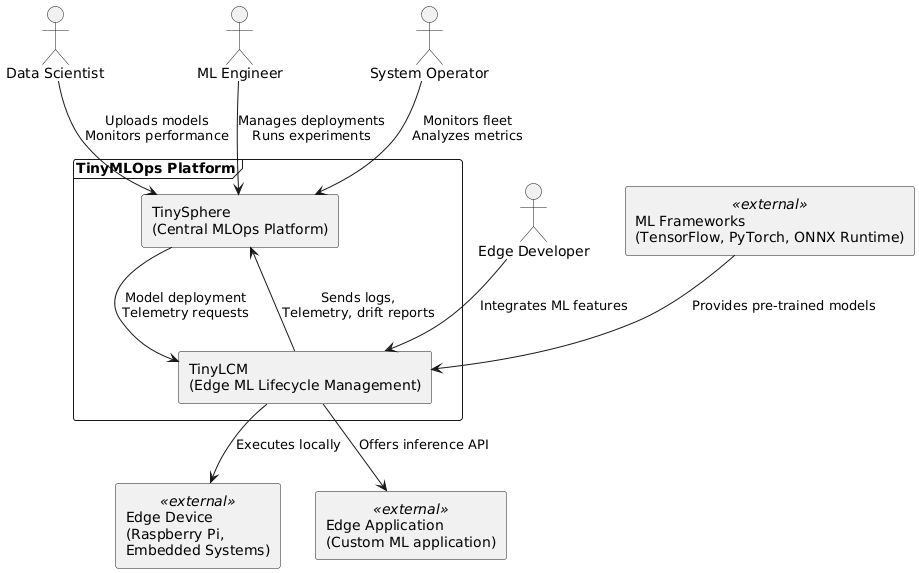
\includegraphics[width=0.75\textwidth]{figs/framework/system-context.png}
    \caption[High-Level System Context Diagram of the TinyMLOps Ecosystem]{High-Level System Context Diagram of the TinyMLOps Ecosystem, illustrating the interaction between Edge Devices (running \gls{tinylcm}) and the TinySphere Server.}
    \label{fig:ecosystem_context_diagram}
\end{figure}

A fundamental characteristic of this architecture is that \gls{tinylcm} is engineered for autonomous on-device \gls{lcm}, even in the complete and prolonged absence of TinySphere. Integration with TinySphere is an enhancement, significantly augmenting edge device capabilities by connecting them to a broader, managed TinyML deployment when circumstances permit. This directly supports FR6, allowing deployments to scale from fully disconnected local autonomy to a comprehensively managed, server-assisted system.


\section{TinyLCM On-Device Framework for Autonomous Lifecycle Management}
\label{sec:tinylcm_detailed_design}

At the core lies \gls{tinylcm}, the on-device framework specifically engineered to endow resource-constrained edge devices with the intelligence and mechanisms required for autonomous \gls{ml} model management. Designed with Python for broad compatibility and leveraging \gls{tfl} for efficient inference, \gls{tinylcm} embodies the ``autonomy-first'' principle of the ecosystem. Its architecture is modular and pipeline-driven, optimized at multiple levels to operate within the severe limitations of hardware such as MCUs and low-power \glspl{sbc}. This section provides a detailed exposition of \gls{tinylcm}'s architectural blueprint, its constituent components, the foundational algorithms for its autonomous drift detection and adaptation capabilities, and the array of resource-optimization tactics employed in its implementation.

\subsection{Architectural Blueprint and Core Components}
\label{ssec:tinylcm_architecture_blueprint}

The internal architecture of \gls{tinylcm} is structured as a pipeline of interconnected, modular components, as illustrated in the component diagram in Figure~\ref{fig:tinylcm_component_diagram}. This design promotes a clear and efficient flow of data and control, from input processing through inference, monitoring, drift detection, and on-device adaptation.

\begin{figure}[htbp]
    \centering
    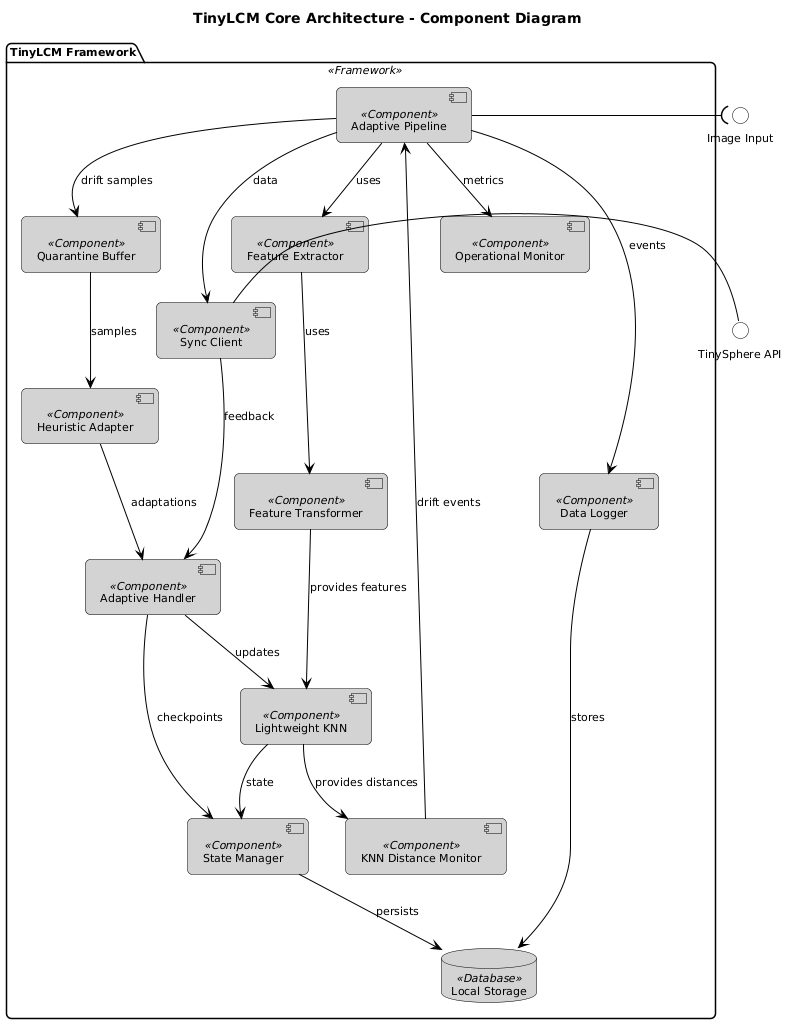
\includegraphics[width=0.65\textwidth]{figs/framework/tinylcm-component-dia.png}
    \caption[Component Diagram of the TinyLCM Core Library]{Component Diagram of the \gls{tinylcm} Core Library, illustrating its main modules and their interdependencies.}
    \label{fig:tinylcm_component_diagram}
\end{figure}

\begin{itemize}
    \item \textit{Pipeline Orchestration (\texttt{AdaptivePipeline}):} This central component, extending a base \texttt{InferencePipeline}, orchestrates the entire on-device workflow. It manages the sequence of operations from data ingestion and feature processing to classification, continuous monitoring, drift detection, and the initiation of adaptation routines.
    \item \textit{Feature Processing Subsystem:} Responsible for transforming raw input data (e.g., images) into a numerical representation suitable for the \gls{ml} model. This subsystem includes the \textit{\texttt{TFLiteFeatureExtractor}}, which utilizes a pre-trained, optimized \gls{tfl} model to extract high-dimensional feature vectors, and the \textit{\texttt{StandardScalerPCATransformer}}, which applies statistical normalization (z-score standardization) and dimensionality reduction to these vectors. The latter step is crucial for reducing computational load and enhancing the performance of subsequent components \cite{disabatoTinyMachineLearning2024}.
    \item \textit{Classification (\texttt{LightweightKNN}):} Performs the primary inference task using an optimized \gls{knn} algorithm, designed for a low memory footprint and computational efficiency. It stores a bounded number of reference samples and provides prediction confidence scores. Its internal state (neighbor distances) is also leveraged by the drift detection mechanism.
    \item \textit{Drift Detection Subsystem (\texttt{KNNDistanceMonitor}):} Implements algorithms for autonomous, on-device drift detection without requiring ground truth labels. The \texttt{KNNDistanceMonitor} tracks the average distance to ``k-nearest neighbors'' in the feature space and employs the Page-Hinkley statistical test to detect significant distributional shifts.
    \item \textit{Adaptation System:} Triggered by the \texttt{AdaptivePipeline} upon drift detection, this system manages the on-device model adaptation process. Key components include the \texttt{QuarantineBuffer}, which temporarily stores input samples flagged by drift detectors or exhibiting anomalous characteristics for analysis or potential use in adaptation; the \texttt{HeuristicAdapter}, which analyzes samples from the \texttt{QuarantineBuffer} and applies heuristic rules (e.g., feature space clustering) to generate pseudo-labels; and the \textit{\texttt{AdaptiveHandler}}, which manages the application of these pseudo-labeled samples to update the on-device model in a controlled manner.
    \item \textit{State Management and Persistence:} Ensures system robustness and recoverability. The \texttt{StateManager} handles versioning and persistent storage (e.g., as JSONL files on an SD card) of critical states, including the classifier's model and reference statistics for drift detectors, enabling rollbacks. The \texttt{DataLogger} records operational logs, inference results, drift events, and adaptation attempts. An \texttt{AdaptationTracker} logs details and outcomes of adaptation events.
    \item \textit{Operational Monitoring (\texttt{OperationalMonitor}):} Continuously tracks on-device performance metrics such as inference latency, CPU utilization, memory usage, and component operational status. This data is valuable for local diagnostics and can be synchronized with TinySphere.
    \item \textit{Synchronization Client (\texttt{SyncClient}):} Manages optional, opportunistic communication with the TinySphere server. This includes packaging data (logs, metrics, drift events, quarantined samples), handling intermittent network connectivity, and processing feedback or updates from the server.
\end{itemize}

This modular and configurable component-based architecture allows \gls{tinylcm} to be adapted to a wide range of applications and hardware platforms, such as \glspl{sbc}.

\subsection{Lightweight KNN Classifier}
\label{ssec:LightweightKNN}

A pivotal component within \gls{tinylcm}, enabling both classification and serving as a basis for drift detection, is the \texttt{LightweightKNN} classifier. This choice is informed by analyses in Chapter~\ref{chp:Research_Results} (specifically Section~\ref{sec:RQ2_Results_Frameworks}) and findings in the literature \cite{disabatoTinyMachineLearning2024} that highlight the suitability of KNN-based approaches for resource-constrained environments due to their potential for low inference cost and incremental updatability.

The \texttt{LightweightKNN} implementation incorporates several critical design decisions and optimizations:
\begin{itemize}
    \item \textit{Bounded Sample Storage for Memory Management:} To prevent uncontrolled memory consumption during long-term operation, the classifier stores its reference feature vectors, corresponding labels, and their arrival timestamps in Python \texttt{collections.deque} objects with a configurable \texttt{maxlen} attribute (\texttt{max\_samples}). This ensures the memory footprint for reference data remains strictly bounded, as oldest samples are automatically evicted when buffer capacity is exceeded—a crucial tactic for RAM optimization.
    \item \textit{Flexible and Efficient Distance Computation:} The classifier supports multiple distance metrics (e.g., Euclidean, Manhattan, Cosine) via a \texttt{DistanceCalculator} utility class. While optimized NumPy calculations are preferred for speed if available and the \texttt{use\_numpy} flag is set, pure Python implementations serve as fallbacks, ensuring broader compatibility.
    \item \textit{Confidence Score Calculation:} For each prediction, a confidence score is calculated. While various schemes exist, such as complex distance-weighting, a common alternative chosen here for stability in drift detection contexts is the simple proportion of votes from the \gls{knn} belonging to the predicted class. This score can be used by downstream components.
    \item \textit{Deterministic Tie-Breaking in Predictions:} In cases where multiple classes receive an equal number of votes among the \gls{knn}, a deterministic tie-breaking mechanism is employed, using sample timestamps. This ensures reproducible prediction outcomes.
    \item \textit{Provision of Neighbor Information for Drift Detection:} A key function is that \texttt{LightweightKNN} makes the distances to, and identities of, the\gls{knn} accessible after each prediction. This internal state is directly consumed by the \texttt{KNNDistanceMonitor}, avoiding redundant distance calculations by the monitor.
\end{itemize}

The core simplified logic, emphasizing efficient distance computation, neighbor selection, and voting, is illustrated in Listing~\ref{lst:lightweightknn_predict}.

\begin{lstlisting}[captionpos=b, language=Python, commentstyle=\color{blue}\itshape, caption={Example logic of the LightweightKNN Class}, label=lst:lightweightknn_predict]
class LightweightKNN:    
    def __init__(self, k=5, max_samples=1000, distance_metric='euclidean'):
        self.samples = deque(maxlen=max_samples)
        self.labels = deque(maxlen=max_samples)
        self.timestamps = deque(maxlen=max_samples)
        self.k = k
        self.distance_metric = distance_metric
        
    def predict(self, features):
        """Predict with neighbor tracking for drift detection."""
        if len(self.samples) < self.k:
            return None, 0.0
            
        # Compute distances efficiently
        distances = self._compute_distances(features)
        
        # Get k nearest neighbors
        k_nearest = sorted(enumerate(distances), key=lambda x: x[1])[:self.k]
        indices = [idx for idx, _ in k_nearest]
        
        # Vote counting with tie-breaking
        label_votes = defaultdict(lambda: {'count': 0, 'min_timestamp': float('inf')})
        for idx in indices:
            label = self.labels[idx]
            label_votes[label]['count'] += 1
            label_votes[label]['min_timestamp'] = min(
                label_votes[label]['min_timestamp'], 
                self.timestamps[idx]
            )
        
        # Determine winner with timestamp tie-breaking
        winner = max(label_votes.items(), 
                    key=lambda x: (x[1]['count'], -x[1]['min_timestamp']))[0]
        
        # Calculate confidence
        confidence = label_votes[winner]['count'] / self.k
        
        # Store neighbor info for drift detection
        self._store_neighbor_info(indices, distances, k_nearest)
        
        return winner, confidence
\end{lstlisting}

\subsection{Autonomous Drift Detection and Adaptation Mechanisms}
\label{ssec:tinylcm_drift_adaptation}

A defining characteristic of \gls{tinylcm}'s on-device \gls{lcm} is its capacity for autonomous concept drift detection and subsequent model adaptation. This approach directly addresses a critical challenge of frequent unavailability of real-time ground truth labels. \gls{tinylcm}'s autonomy is realized through an integrated system of statistical feature-space monitoring and heuristic-driven learning mechanisms, orchestrated within the \texttt{AdaptivePipeline}.

\paragraph{KNN-Distance Monitoring with Page-Hinkley Test}
Traditional drift detection methods often depend on true labels to monitor model performance \cite{disabatoTinyMachineLearning2024, pavanTyBoxAutomaticDesign2024}. \gls{tinylcm} therefore employs unsupervised drift detection by monitoring the statistical properties of input data within a learned feature space. The premise is that concept drift—a change in $P(X)$ or $P(Y|X)$ \cite{gamaSurveyConceptDrift2014}—often manifests as a discernible shift in how new data relates to an established reference distribution.

The process begins with the \texttt{TFLiteFeatureExtractor} transforming raw input data into a high-dimensional feature space. These features are then processed by the \texttt{StandardScalerPCATransformer}, which applies L2-normalization (Equation~\ref{eq:l2_norm_chap5_v2}), z-score standardization (Equation~\ref{eq:z_score_chap5_v2}), and PCA (Equation~\ref{eq:pca_transform_chap5_v2}). This pipeline, for instance, can reduce feature vectors from 1280 to 256 dimensions, normalizing feature scales and mitigating the curse of dimensionality, thereby enhancing the robustness of distance-based metrics used subsequently \cite{jolliffePrincipalComponentAnalysis2016}. The selection of these techniques aligns with common practices in \gls{tinyml} for preprocessing data efficiently, as discussed in Chapter~\ref{chp:Research_Results} concerning data-centric architectures.

Within this transformed, lower-dimensional feature space, the \texttt{LightweightKNN} classifier (Section~\ref{ssec:LightweightKNN}) provides not only predictions but also the Euclidean distances to the $k$-nearest neighbors for each query point (Equation~\ref{eq:euclidean_distance_chap5_v2}). The \texttt{KNNDistanceMonitor} component utilizes the average of these $k$ distances, denoted $x_t$ (Equation~\ref{eq:drift_signal_chap5_v2}), as a sensitive proxy metric. A statistically significant, sustained increase in $x_t$ suggests incoming data points are becoming dissimilar to the reference data, indicating a potential distribution shift.

To formally detect such changes, the \texttt{KNNDistanceMonitor} employs the Page-Hinkley test \cite{pageContinuousInspectionSchemes1954}, a sequential analysis technique well-suited for detecting persistent changes in a signal's mean. Given the time series of average \gls{knn} distances $x_t$, a reference mean distance $\mu_0$ (established during an initial warm-up phase), and a tolerance parameter $\delta > 0$, the Page-Hinkley test statistics are updated incrementally (Equations~\ref{eq:ph_mt_chap5_v2} through \ref{eq:ph_statistic_chap5_v2}).

Let \(\mathbf{f}_{\mathrm{raw}}\in\mathbb{R}^D\) denote the raw feature vector. L\(^2\)-normalization yields:
\begin{flalign}
  && \mathbf{f}_{\mathrm{norm}}
   = \frac{\mathbf{f}_{\mathrm{raw}}}{\|\mathbf{f}_{\mathrm{raw}}\|_2},
  \qquad
  \|\mathbf{f}_{\mathrm{raw}}\|_2
   = \sqrt{\sum_{i=1}^D f_{\mathrm{raw},i}^2}. &&
   \label{eq:l2_norm_chap5_v2}
\end{flalign}
Standardization and PCA transformation follow:
\begin{flalign}
  && \mathbf{z}
   = \frac{\mathbf{f}_{\mathrm{norm}} - \boldsymbol{\mu}_{\mathrm{norm}}}
         {\boldsymbol{\sigma}_{\mathrm{norm}}}, &&
   \label{eq:z_score_chap5_v2}\\
  && \mathbf{y}
   = \mathbf{z}\,W,
  \qquad
  \mathbf{y}\in\mathbb{R}^K. &&
   \label{eq:pca_transform_chap5_v2}
\end{flalign}
The Euclidean distance to a neighbor $\mathbf{r}_j$ for a point $\mathbf{y}_t$ is:
\begin{flalign}
  && d(\mathbf{y}_t,\mathbf{r}_j)
   = \sqrt{\sum_{i=1}^K \bigl(y_{t,i} - r_{j,i}\bigr)^2}, &&
   \label{eq:euclidean_distance_chap5_v2}
\end{flalign}
leading to the average KNN distance (drift signal):
\begin{flalign}
  && x_t = \frac{1}{k}\sum_{j=1}^k d(\mathbf{y}_t,\mathbf{r}_j). &&
   \label{eq:drift_signal_chap5_v2}
\end{flalign}
The Page-Hinkley test statistics are then:
\begin{flalign}
  && m_t = m_{t-1} + \bigl(x_t - \mu_0 - \delta\bigr), \quad \text{with } m_0 = 0, &&
   \label{eq:ph_mt_chap5_v2}\\
  && M_t = \min\bigl(M_{t-1},\,m_t\bigr), \quad \text{with } M_0 = 0, &&
   \label{eq:ph_Mt_chap5_v2}\\
  && PH_t = m_t - M_t. &&
   \label{eq:ph_statistic_chap5_v2}
\end{flalign}

A drift is flagged if $PH_t$ exceeds a predefined detection threshold $\lambda$. The operational flow of the \texttt{KNNDistanceMonitor}, including hysteresis and cooldown periods to prevent alarm flooding—a practical consideration for stable autonomous systems is detailed in Algorithm~\ref{alg:knn_distance_monitor_update}.

\begin{algorithm}[htbp]
  \caption{Update procedure for the \texttt{KNNDistanceMonitor}}
  \label{alg:knn_distance_monitor_update}
  \begin{algorithmic}[1]
    \Require Current average KNN distance $x_t$; Reference mean $\mu_0$; Tolerance $\delta$; Detection threshold $\lambda$; Exit threshold $\lambda_{\mathrm{exit}}$; Current Page-Hinkley sums $m_{t-1}, M_{t-1}$; Warm-up data buffer $W$; Warm-up phase flag $is\_warmup$; Reference initialized flag $ref\_initialized$; In drift state flag $in\_drift\_state$.
    \If{$is\_warmup$}
      \State Add $x_t$ to $W$.
      \State \Return \textbf{no drift}
    \ElsIf{not $ref\_initialized$}
      \State $\mu_0 \gets \mathrm{mean}(W)$; $\sigma_0 \gets \mathrm{std}(W)$ \Comment{Initialize reference from warm-up data}
      \State $m_t \gets 0$; $M_t \gets 0$ \Comment{Initialize Page-Hinkley statistics}
      \State $ref\_initialized \gets \textbf{true}$
      \State \Return \textbf{no drift}
    \Else
      \State $m_t \gets m_{t-1} + (x_t - \mu_0 - \delta)$
      \State $M_t \gets \min(M_{t-1}, m_t)$
      \State $PH_t \gets m_t - M_t$
      \If{not $in\_drift\_state$ and $PH_t > \lambda$}
        \State $in\_drift\_state \gets \textbf{true}$
        \State \Return \textbf{drift detected}
      \ElsIf{$in\_drift\_state$ and $PH_t \le \lambda_{\mathrm{exit}}$}
        \State $in\_drift\_state \gets \textbf{false}$
        \State $m_t \gets 0$; $M_t \gets 0$ \Comment{Reset Page-Hinkley statistics}
        \State \Return \textbf{drift ended}
      \Else
        \State \Return \textbf{no drift (or still in drift)}
      \EndIf
    \EndIf
  \end{algorithmic}
\end{algorithm}
\FloatBarrier

\paragraph{Heuristic Pseudo-Labeling and Quarantine}
Upon significant drift detection, \gls{tinylcm}'s \texttt{AdaptivePipeline} initiates an on-device adaptation process. This process, depicted in Figure~\ref{fig:heuristic_adaptation_sequence_diagram}, is engineered for immediate yet cautious response. It leverages a heuristic-based pseudo-labeling strategy to update the on-device model, aiming for adaptation without requiring immediate external ground truth. This contrasts with more resource-intensive on-device retraining approaches discussed in Chapter~\ref{chp:Research_Results} (e.g., full backpropagation), and is chosen for its balance of responsiveness and computational frugality, suitable for \glspl{mcu}.

\begin{figure}[htbp]
    \centering
    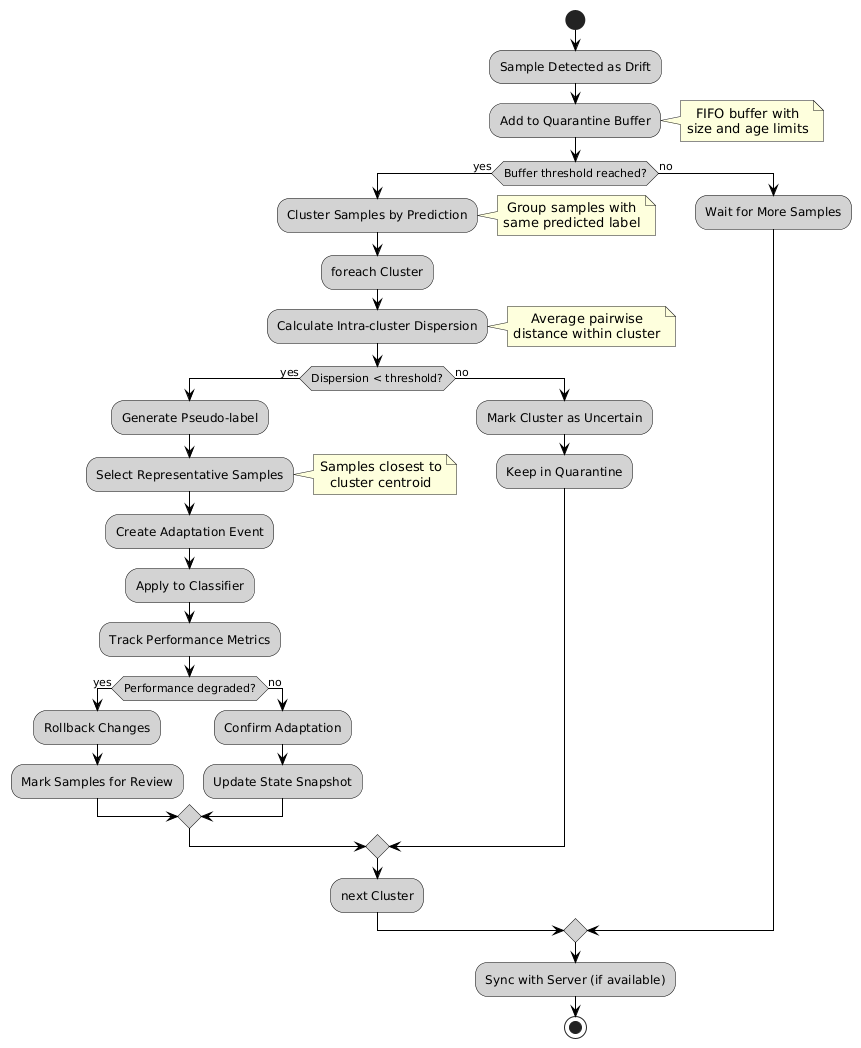
\includegraphics[width=0.75\textwidth]{figs/framework/heuristic-adaptation-activity.png}
    \caption[Activity Diagram of the Heuristic Adaptation Process]{Activity Diagram detailing the heuristic adaptation logic}
    \label{fig:heuristic_adaptation_sequence_diagram}
\end{figure}
\FloatBarrier

The on-device adaptation cycle involves the following stages:
\begin{itemize}
    \item \textit{Quarantine Buffer Management:} Input samples triggering a drift alert, or subsequent samples with similar anomalous characteristics, are moved to the \texttt{QuarantineBuffer}. This FIFO buffer, with configurable size and sample age limits, collects a small, manageable set of these ``unusual'' samples for focused analysis.
    \item \textit{Heuristic Pseudo-Labeling by \texttt{HeuristicAdapter}:} The \texttt{HeuristicAdapter} analyzes feature vectors of samples in the \texttt{QuarantineBuffer}. A core heuristic involves clustering these quarantined samples within their PCA-transformed feature space. Samples might be grouped based on their original (potentially incorrect) \texttt{LightweightKNN} prediction or via unsupervised clustering if no prior prediction is reliable. If a sufficiently distinct and cohesive cluster of new, anomalous samples forms, it may be inferred that these samples represent a novel or significantly shifted concept. A pseudo-label is then assigned (e.g., based on the predominant original label if cohesive, or a new ``unknown'' label if distinct). Confidence in such pseudo-labels can be derived from metrics like intra-cluster dispersion, cluster size, and separation from existing class centroids.
    \item \textit{Cautious Model Update via \texttt{AdaptiveHandler}:} Adaptation events, containing representative samples from a confident pseudo-labeled cluster, are passed to the \texttt{AdaptiveHandler}. This component cautiously updates the \texttt{LightweightKNN} classifier by adding these pseudo-labeled samples to its reference set.
    \item \textit{Post-Adaptation Performance Monitoring and Rollback:} Following adaptation, the \texttt{AdaptiveHandler} and \texttt{OperationalMonitor} continue to track performance. If metrics indicate performance degradation, a rollback to the previously saved state can be automatically triggered via the \texttt{StateManager}. Samples causing detrimental adaptation may be flagged for mandatory server review.
    \item \textit{Opportunistic External Validation:} Pseudo-labeled samples, their generation context, and adaptation outcomes are packaged by the \texttt{SyncClient}. This package is queued for optional, asynchronous transmission to TinySphere when connectivity permits. TinySphere can then employ more sophisticated validation (e.g., human-in-the-loop analysis) to confirm/refute pseudo-labels. This validated feedback can subsequently refine \gls{tinylcm} models during future synchronizations, aligning with the concept of the Active/Passive handlers used in \cite{disabatoIncrementalOnDeviceTiny2020,disabatoTinyMachineLearning2024}.
\end{itemize}

This adaptive loop—combining autonomous detection, heuristic-based learning, robust state management, and optional external validation—allows \gls{tinylcm} to dynamically evolve its understanding of the operational environment and maintain performance despite changing data distributions, a key aspect of robust \gls{lcm} practices discussed as emerging in Chapter~\ref{chp:Research_Results}.

\begin{MyBox}{\textbf{Implementation Status of On-Device Heuristic Adaptation}}
    It is important to note that the on-device heuristic pseudo-labeling and adaptation logic described represents a conceptual and architectural design developed for this thesis. While the overall workflow and component interactions (e.g., with the \texttt{QuarantineBuffer} and \texttt{AdaptiveHandler}) are defined, the specific algorithms for heuristic pseudo-label generation and their efficient, resource-aware implementation have not yet been fully realized and tested.
\end{MyBox}

\paragraph{State Management for Resilience}
To ensure operational resilience, particularly when autonomous adaptations may not consistently yield improvements, \gls{tinylcm} incorporates a robust \texttt{AdaptiveStateManager}. This component is crucial because on-device adaptations, while aiming to maintain performance in dynamic environments, risk issues such as catastrophic forgetting or incorrect learning from noisy data, especially when ground truth is absent \cite{renOndeviceOnlineLearning2024, pavanTyBoxAutomaticDesign2024}. The \texttt{AdaptiveStateManager} mitigates these risks by versioning the state of critical components, primarily the \texttt{LightweightKNN} classifier's reference set (features, labels, and timestamps), enabling rollbacks to known-good configurations.

The core mechanism involves saving the classifier's current state \textit{before} any on-device adaptation is applied. This snapshot, including the KNN's reference samples, a version identifier, and a timestamp, is serialized to non-volatile storage. A key consideration for resource-constrained devices is the performance impact of this save operation. Therefore, as illustrated in Listing~\ref{lst:statemanager}, this operation is handled asynchronously using a dedicated worker thread and task queue. This non-blocking approach prevents the main inference pipeline from stalling.

If subsequent evaluation—either through \gls{tinylcm}'s on-device monitoring of proxy metrics or via feedback from TinySphere (Section~\ref{sec:tinysphere_detailed_design})—indicates that an adaptation has degraded performance, a rollback is triggered. The \texttt{AdaptiveStateManager} then restores the \texttt{LightweightKNN} classifier to its previously saved, validated state. To manage limited storage resources effectively, the state manager also implements a policy for pruning old or superseded snapshots.

\begin{lstlisting}[captionpos=b, language=Python, commentstyle=\color{blue}\itshape, caption={\texttt{AdaptiveStateManager} Implementation Highlights}, label=lst:statemanager]
class AdaptiveStateManager:
    
    def __init__(self, storage_path: Path, max_snapshots: int = 10):
        self.storage_path = storage_path
        self.max_snapshots = max_snapshots
        self.worker_thread = Thread(target=self._worker, daemon=True)
        self.task_queue = Queue()
        self.worker_thread.start()
        
    def create_snapshot(self, pipeline_state: dict, metadata: dict):
        """Create state snapshot asynchronously."""
        snapshot = {
            'timestamp': datetime.now().isoformat(),
            'state_version': 2,
            'pipeline_state': pipeline_state,
            'metadata': metadata
        }
        
        self.task_queue.put(('save', snapshot))
        
    def rollback_to_snapshot(self, snapshot_id: str) -> dict:
        """Restore system state from snapshot."""
        snapshot_path = self.storage_path / f"{snapshot_id}.json"
        with open(snapshot_path, 'r') as f:
            snapshot = json.load(f)
            
        if snapshot['state_version'] != 2:
            raise ValueError(f"Incompatible state version: {snapshot['state_version']}")
            
        return snapshot['pipeline_state']
\end{lstlisting}

\section{TinySphere: A TinyML-Centric Server Platform for Enhanced MLOps}
\label{sec:tinysphere_detailed_design}

While \gls{tinylcm} provides the foundational layer for on-device autonomy, the TinySphere platform serves as its optional, yet deeply integrated, server-side counterpart. TinySphere is specifically architected to extend traditional \gls{mlops} capabilities, such as those offered by MLflow, with functionalities tailored to the unique operational lifecycle and data characteristics of fleets of adaptive \gls{tinyml} devices. It is not merely a generic \gls{mlops} backend but a purposeful extension designed to seamlessly integrate with \gls{tinylcm}-enabled devices, understand their autonomously generated data, and provide a centralized hub for validation, monitoring, advanced analytics, and fleet management. This section outlines the rationale for TinySphere, details its architectural design, and highlights its key contributions to the comprehensive TinyMLOps ecosystem.

\subsection{Rationale and Objectives for a TinyML-Centric MLOps Platform}
\label{ssec:tinysphere_rationale}

The imperative for developing TinySphere stems from the observation, articulated in Section~\ref{ssec:framework_revisiting_gaps}, that existing \gls{mlops} platforms often fall short when addressing the specific needs of managing autonomous, adaptive fleets of TinyML devices operating at the extreme edge. While powerful tools like Edge Impulse excel in the initial model development and deployment phases \cite{banburyEdgeImpulseMLOps2023}, and platforms such as MLflow provide robust components for generic experiment tracking and model versioning in conventional ML workflows \cite{condeEnhancedFIWAREBasedArchitecture2024}, a dedicated platform is required to effectively:
\begin{itemize}
    \item \textit{TinyML-Specific Data Streams:} Handle the unique data packages originating from \gls{tinylcm}-enabled devices, which include drift events detected via proxy metrics, heuristically generated pseudo-labels, on-device adaptation logs, and resource-constrained operational telemetry.
    \item \textit{Asynchronous Validation of On-Device Decisions:} Provide mechanisms for the external, potentially human-in-the-loop, validation of autonomous on-device adaptations. This is crucial for ensuring the long-term reliability and correctness of unsupervised learning processes occurring at the edge.
    \item \textit{Enable Centralized Monitoring and Comparative Analytics:} Aggregate operational data from a distributed fleet of resource-constrained devices to provide a centralized overview of system health, model performance across diverse environments, and emergent drift patterns.
    \item \textit{Tailored Model Management and Deployment Strategies:} Support model management and deployment workflows that explicitly account for the severe constraints (e.g., limited bandwidth, intermittent connectivity, heterogeneous hardware) and unique update mechanisms (e.g., \gls{tinylcm}'s model pull strategy) of TinyML targets.
    \item \textit{Edge Autonomy with Centralized Oversight:} Create a unified \gls{lcm} framework that respects and leverages on-device autonomy while providing the benefits of centralized MLOps for tasks where scale, computational power, or human expertise are indispensable.
\end{itemize}

\subsection{Architectural Design of TinySphere}
\label{ssec:tinysphere_architecture}

TinySphere is implemented as a modern, microservices-oriented web application. Its backend is built using FastAPI, chosen for its high performance, asynchronous capabilities, and automatic OpenAPI documentation generation, providing a robust and scalable RESTful API for communication with \gls{tinylcm} clients and the web dashboard. For data persistence, TinySphere employs a dual-storage strategy: (i) a PostgreSQL database is utilized for storing structured relational data, such as device metadata, drift event summaries, package information, and processed metrics; (ii) MinIO, an S3-compatible object storage solution, is used for managing larger binary artifacts, including uploaded device packages, images associated with drift events, full operational logs, and model files.

A cornerstone of TinySphere's design is its extension of, and integration with, MLflow. Rather than reinventing established MLOps components, TinySphere leverages MLflow for core functionalities like experiment tracking and model registry, while building specialized TinyML-centric services around it. The overall architecture, illustrated in Figure~\ref{fig:tinysphere_architecture_diagram}, delineates the API layer, service layer, data persistence layer, and its interaction with external systems and the edge devices.

\begin{figure}[htbp]
    \centering
    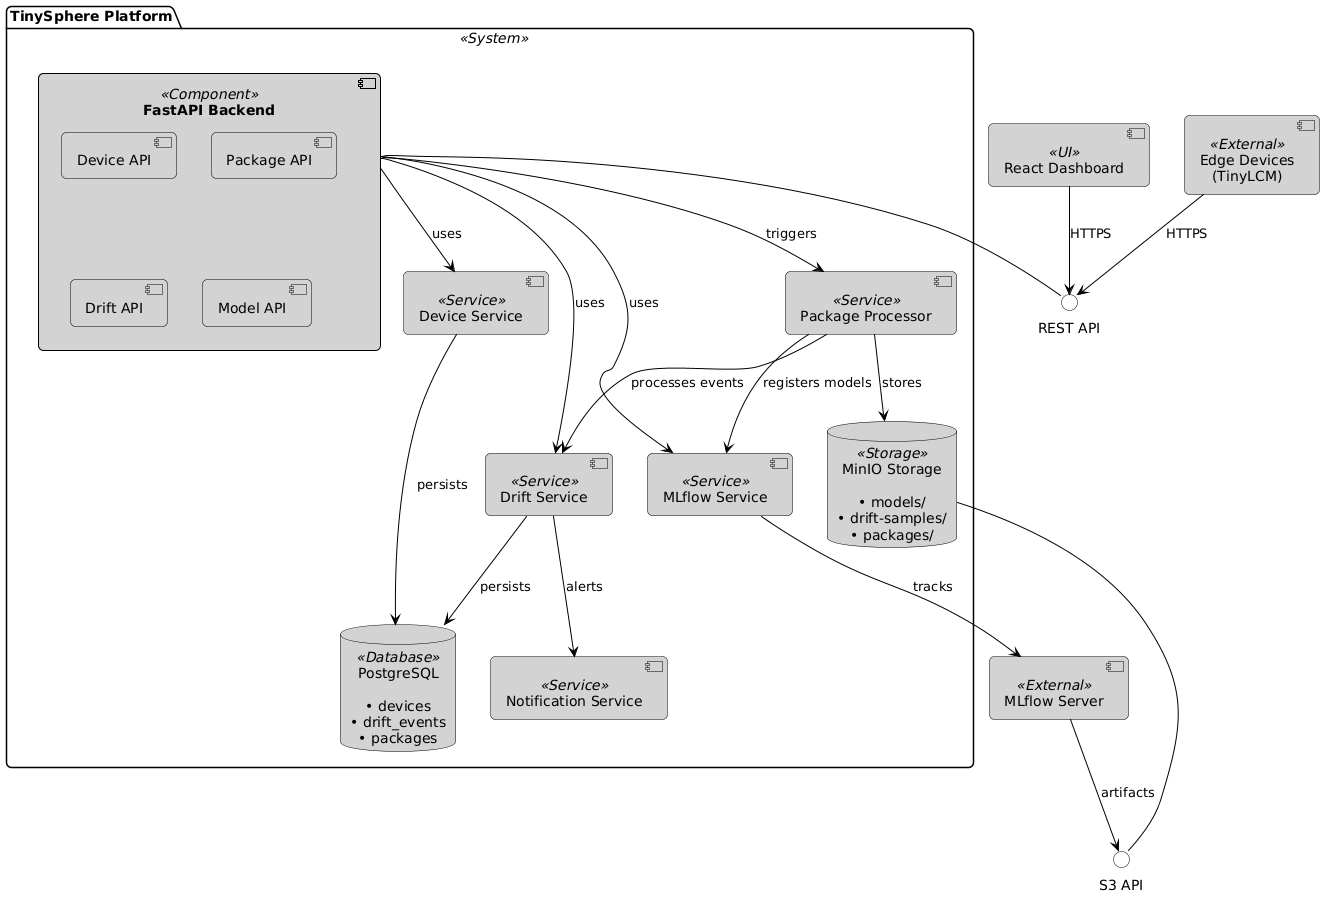
\includegraphics[width=0.95\textwidth]{figs/framework/tinysphere-architecture.png}
    \caption[Architectural Design of the TinySphere Server Platform]{Architectural Component Diagram of the TinySphere Server Platform}
    \label{fig:tinysphere_architecture_diagram}
\end{figure}

Key architectural components within TinySphere include:
\begin{itemize}
    \item \textit{API Layer}: Provides RESTful endpoints for all external interactions. This includes distinct routers for device management (`Device API`), package uploads and processing (`Package API`), drift event querying and validation (`Drift API`), and model management interactions (`Model API`).
    \item \textit{MLflow Service}: Orchestrates interactions with the MLflow tracking server and model registry, for example, when processing model-related information from device packages or logging server-side (re)training experiments.
    \item \textit{Drift Service}: Manages the lifecycle of drift events reported by devices, from initial ingestion and storage of associated samples and metadata to facilitating their validation workflow and tracking resolution status.
    \item \textit{Device Service}: Handles device registration, maintains a registry of active devices, tracks their status (e.g., connectivity, platform details, \gls{tinylcm} version), and manages associated metadata such as geolocation.
    \item \textit{Package Processor}: An extensible, multi-stage pipeline responsible for receiving, extracting, and processing the diverse data packages uploaded by \gls{tinylcm} devices. It detects package types (e.g., model, metrics, drift, operational logs) and routes their contents to appropriate transformers and services for storage and analysis.
    \item \textit{PostgreSQL Database}: Stores structured, relational data, including device registry, drift event metadata, package tracking information, and aggregated metrics for dashboarding.
    \item \textit{MinIO Object Storage}: Provides scalable storage for binary artifacts, such as original uploaded packages, extracted drift samples (images, features), model files, and extensive operational logs.
    \item \textit{Frontend (Web Dashboard)}: A React-based web application, providing an interactive interface for ML engineers and data scientists to monitor the device fleet, manage devices, review and validate drift events, inspect operational data, and interact with the model registry. An iullustrative mockup of this interface is shown in Figure~\ref{fig:uitinysphere}.
\end{itemize}

\subsection{Key MLOps Capabilities Provided by TinySphere}
\label{ssec:tinysphere_capabilities}

TinySphere is designed to deliver a suite of MLOps capabilities, extending the autonomous operations of \gls{tinylcm}-enabled devices:

\begin{itemize}
    \item \textit{Package Processing and Data Transformation}: TinySphere's `PackageProcessor` implements a sophisticated pipeline that can automatically detect the type of incoming data packages from \gls{tinylcm} devices and route them to a series of appropriate data transformers. For example, a `ModelTransformer` might register a new on-device model version with MLflow and store its artifact in MinIO; a `MetricsTransformer` could extract performance data and log it as an MLflow experiment/run; a `DriftTransformer` processes drift event details and stores associated samples for review; and an `OperationalLogsTransformer` parses raw log entries for aggregation and analysis. This automated pipeline, illustrated in Figure~\ref{fig:package_processing_pipeline}, ensures that data from the edge is efficiently ingested, processed, and made available for various MLOps workflows.

    \begin{figure}[htbp]
        \centering
        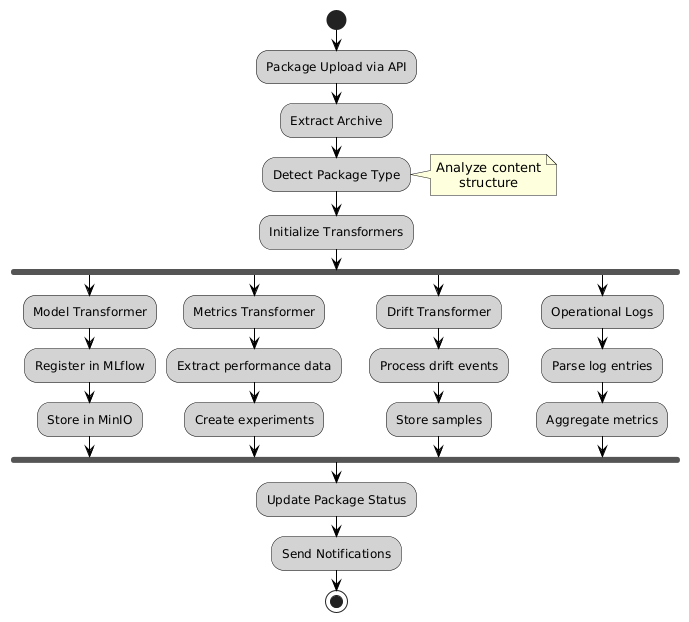
\includegraphics[width=0.7\textwidth]{figs/framework/package-processing-pipeline.png}
        \caption[Package Processing Pipeline in TinySphere]{Activity Diagram of the TinySphere Package Processing Pipeline}
        \label{fig:package_processing_pipeline}
    \end{figure}

    \item \textit{Drift Management}: TinySphere provides a dedicated system for managing and validating drift events. It supports various drift types (confidence-based, distribution-based, KNN-distance based). Reported drift samples are stored in MinIO, allowing human experts to review them via the TinySphere dashboard (``Drift Hub''). A structured validation workflow, depicted in Figure~\ref{fig:drift_validation_workflow}, enables experts to provide ground truth labels or confirm/reject on-device heuristic adaptations. This validated feedback, can then be synchronized back to the edge devices, facilitating a closed-loop learning process that refines on-device models with high-quality supervisory signals.

    \begin{figure}[htbp]
        \centering
        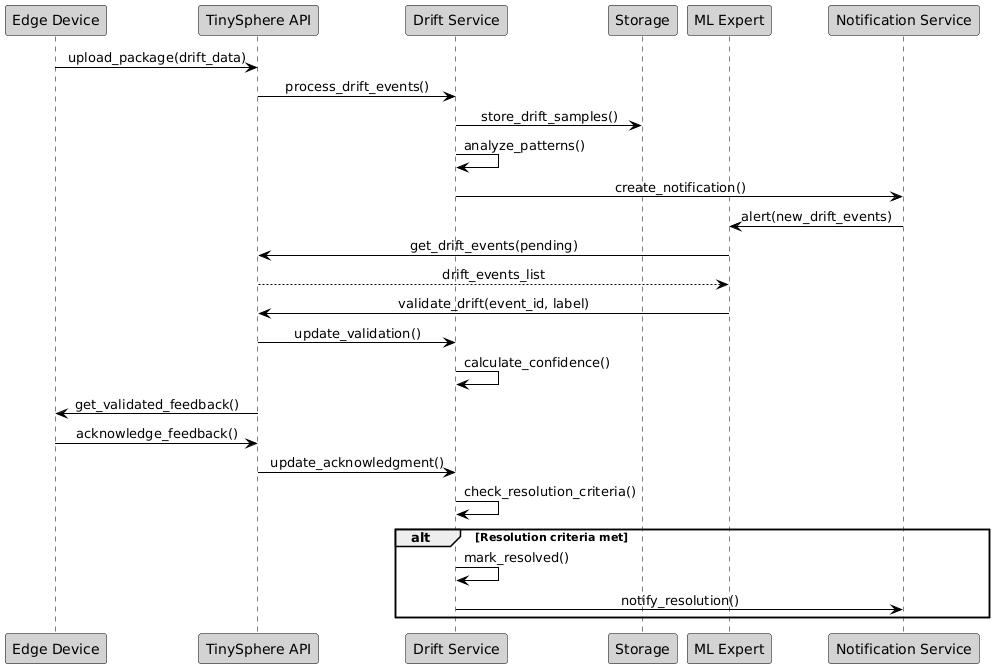
\includegraphics[width=0.9\textwidth]{figs/framework/drift-validation-workflow.png}
        \caption[Drift Validation Workflow in TinySphere]{Sequence Diagram illustrating the Drift Validation Workflow in TinySphere}
        \label{fig:drift_validation_workflow}
    \end{figure}

    \item \textit{Device Fleet Management}: The ``DeviceService'' within TinySphere maintains a registry of all connected \gls{tinylcm} devices, tracking their operational status, platform details (OS, \gls{tinylcm} version), connectivity (e.g., ``online'', ``offline'' based on last seen time), and, if provided by the device, geolocation data. This enables fleet-wide monitoring and allows for the correlation of model performance or drift occurrences with specific geographical regions or environmental contexts, visualized on the dashboard.

    \item \textit{Model Registry}: TinySphere seamlessly integrates with an MLflow server for its model registry capabilities. Models trained or fine-tuned based on fleet data, or even new base models intended for deployment, can be registered in MLflow. TinySphere extends this by associating TinyML-specific metadata with these models, such as their quantized size, target platform suitability, typical inference time on reference edge hardware, and configurations for associated feature extractors or drift detectors.
    \item \textit{Operational Monitoring}: By aggregating metrics and logs from \gls{tinylcm} devices, TinySphere provides a centralized dashboard for monitoring overall system health of deployed models.
\end{itemize}
These capabilities collectively position TinySphere as a specialized MLOps control plane, designed to augment the autonomy of \gls{tinylcm}-powered edge devices with robust, scalable, and insightful server-side operational management. Example mockups of the TinySphere user interface are provided in Figure~\ref{fig:uitinysphere}.

\begin{figure}[htbp]
    \centering
    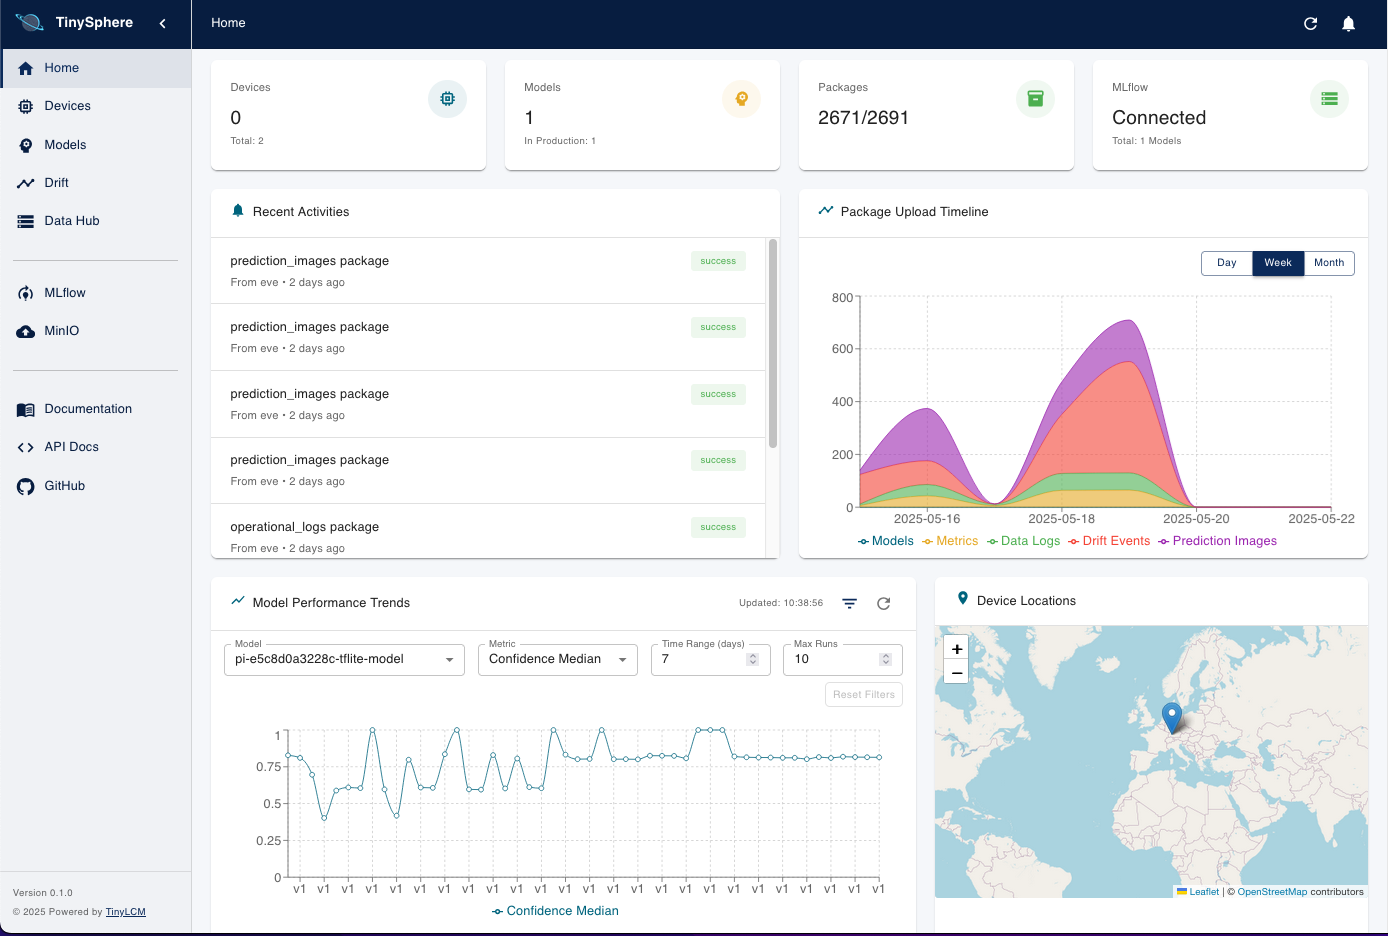
\includegraphics[width=0.975\textwidth]{figs/framework/ui-tinyssphere.png}
    \caption[User Interface of TinySphere]{User Interface of TinySphere, illustrating the dashboard for monitoring device status and drift events.}
    \label{fig:uitinysphere}
\end{figure}

\begin{MyBox}{\textbf{Note on TinySphere's Interaction with Conceptual Heuristic Adaptation}}
    Further to the implementation status of the on-device heuristic adaptation logic within \gls{tinylcm} (as noted in Section~\ref{sec:tinylcm_detailed_design}), it is important to reiterate that TinySphere's capabilities for processing, validating, and providing feedback on data originating from these specific adaptations are, by extension, also based on this conceptual foundation.
\end{MyBox}

\section{Exemplary Operational Workflow}
\label{ssec:ecosystem_workflow}

To illustrate the practical application and collaborative nature of the TinyMLOps ecosystem based on its current implementation state, this subsection outlines an exemplary end-to-end operational workflow. This workflow, particularly relevant for the Proof-of-Concept development (the Mars rover prototype), spans from initial local model development to continuous production operation involving on-device drift detection and server-assisted data analysis. The workflow is divided into three main phases, detailed below.

\textbf{Phase 1: Local Development and Initial Model Training}
The initial creation of the \gls{ml} model and essential \gls{tinylcm} artifacts occurs on a development machine, forming the foundation for edge deployment.
\begin{enumerate}
    \item \textit{Model Prototyping and Training:} An \gls{ml} engineer utilizes scripts (e.g., Python scripts leveraging TensorFlow/Keras) to perform transfer learning, typically using a pre-trained base model such as MobileNetV2, on a custom dataset relevant to the target application. This process culminates in a quantized \gls{tfl} model optimized for edge deployment, along with associated class labels.
    \item \textit{Feature Processor Generation:} Concurrently, the feature processing pipeline components, including the \texttt{StandardScaler} and \texttt{PCA} models, are fitted on features extracted from the training dataset. These fitted transformers are saved for on-device deployment.
    \item \textit{Initial State Generation for \gls{tinylcm}:} Specialized scripts are executed to create the initial state for the \texttt{LightweightKNN} classifier by populating it with a representative subset of the training data. Additionally, initial reference statistics for the \texttt{KNNDistanceMonitor} are computed based on the trained model and feature processor.
    \item \textit{Configuration File Preparation:} A scenario-specific JSON configuration file is meticulously prepared. This file defines paths to all necessary artifacts (model, scaler, PCA model, initial KNN state, labels) and specifies operational parameters for all \gls{tinylcm} components, including the feature extractor, classifier, drift detectors, and \texttt{SyncClient}.
    \item \textit{Version Control and Packaging:} All generated artifacts, configuration files, \gls{tinylcm} library code, and application-specific scripts are committed to a version control system (e.g., Git) and packaged for deployment.
\end{enumerate}

\textbf{Phase 2: Device Deployment and Autonomous Drift Detection}
Provisioning the target edge device and initiating \gls{tinylcm}'s autonomous operational loop—focused on inference and drift detection—constitute the second phase.
\begin{enumerate}
    \item \textit{Edge Device Preparation:} The target edge device is prepared with a suitable base operating system and necessary system dependencies.
    \item \textit{Installation and Setup:} The device executes an installation script fetched from the Git repository via `curl`. This script automates cloning the application repository, installing Python dependencies, copying specific scenario files to appropriate device locations, and establishing the directory structure for logs and state persistence.
    \item \textit{Initiation of Autonomous Execution:} The main application script is launched on the device. \gls{tinylcm}, configured via the JSON file, commences its autonomous operational loop: performing inference on input data; continuously monitoring for concept drift; and, if drift is detected, quarantining the relevant raw input samples and logging detailed event information using the \texttt{QuarantineBuffer} and \texttt{DataLogger}.
\end{enumerate}

\textbf{Phase 3: TinySphere Integration and Data Review for MLOps}
Synergistic interaction with TinySphere for enhanced \gls{mlops} capabilities, assuming opportunistic network connectivity, characterizes the third phase.
\begin{enumerate}
    \item \textit{Opportunistic Data Synchronization:} If configured to communicate with a TinySphere instance and network connectivity is available, \gls{tinylcm}'s \texttt{SyncClient} periodically (or upon specific triggers, such as a significant drift event) packages locally buffered data. This data includes operational logs, performance metrics, detailed drift event information, and the quarantined raw input samples associated with detected drift. These packages are then transmitted to the TinySphere API.
    \item \textit{Data Ingestion and Processing:} TinySphere's backend API receives these packages. Its \texttt{PackageProcessor} component validates, extracts, and routes the contained data to various specialized services and transformers. Operational logs and metrics are parsed for dashboard visualization. Drift event details and the associated raw samples are processed by a \texttt{DriftTransformer} and stored (e.g., images in MinIO, metadata in PostgreSQL), making them accessible via TinySphere's ``Data Hub'' (or ``Drift Hub'') interface for review by an \gls{ml} engineer.
    \item \textit{MLflow Integration for Experiment and Model Tracking:} An \texttt{MLflowService} within TinySphere can be used to log experiment runs related to model performance observed on devices. While on-device adaptations are not occurring, data from drift events or device telemetry can inform the tracking of deployed model behavior over time. New centrally trained model versions can be registered, with artifacts stored (e.g., in MinIO).
    \item \textit{Fleet Management, Monitoring, and Data Review:} \gls{ml} engineers and data scientists can utilize the TinySphere web interface (illustrative examples in Figure~\ref{fig:tinysphere_ui_examples}) to monitor the operational status of registered devices, view aggregated performance analytics, and, crucially, examine the quarantined raw samples and detailed drift events from across the fleet within the ``Data Hub''.
    \item \textit{Manual Data Labeling and Analysis:} Through the ``Data Hub'' UI, human operators can review the quarantined raw samples (e.g., images of unknown objects or inputs that triggered drift alerts) associated with drift events reported by devices. They can then manually assign ground truth labels to these samples. This manually labeled dataset becomes a valuable asset, stored by TinySphere.
    \item \textit{Model Improvement Cycle:} The manually labeled data, aggregated in TinySphere from various devices and drift events, serves as a curated dataset for model analysis and retraining. An \gls{ml} engineer can use this dataset to: (i) understand the nature of the drift, (ii) augment the training dataset, and (iii) trigger a central retraining cycle for the \texttt{LightweightKNN} or even the base feature extractor model. A new, improved model version, once validated centrally, can then be packaged (Phase 1) and subsequently deployed to the edge device(s) through an appropriate update mechanism (e.g., manual update, or a future automated deployment feature of TinySphere).
\end{enumerate}

This workflow, emphasizing on-device drift detection and server-assisted data collection for human-driven analysis and model evolution, demonstrates a pragmatic approach to managing TinyML applications and addresses operational complexities identified in Chapter~\ref{chp:Research_Results} within the bounds of the current implementation.

\begin{figure}[htbp]
    \centering

    \begin{subfigure}[b]{0.48\textwidth}
        \centering
        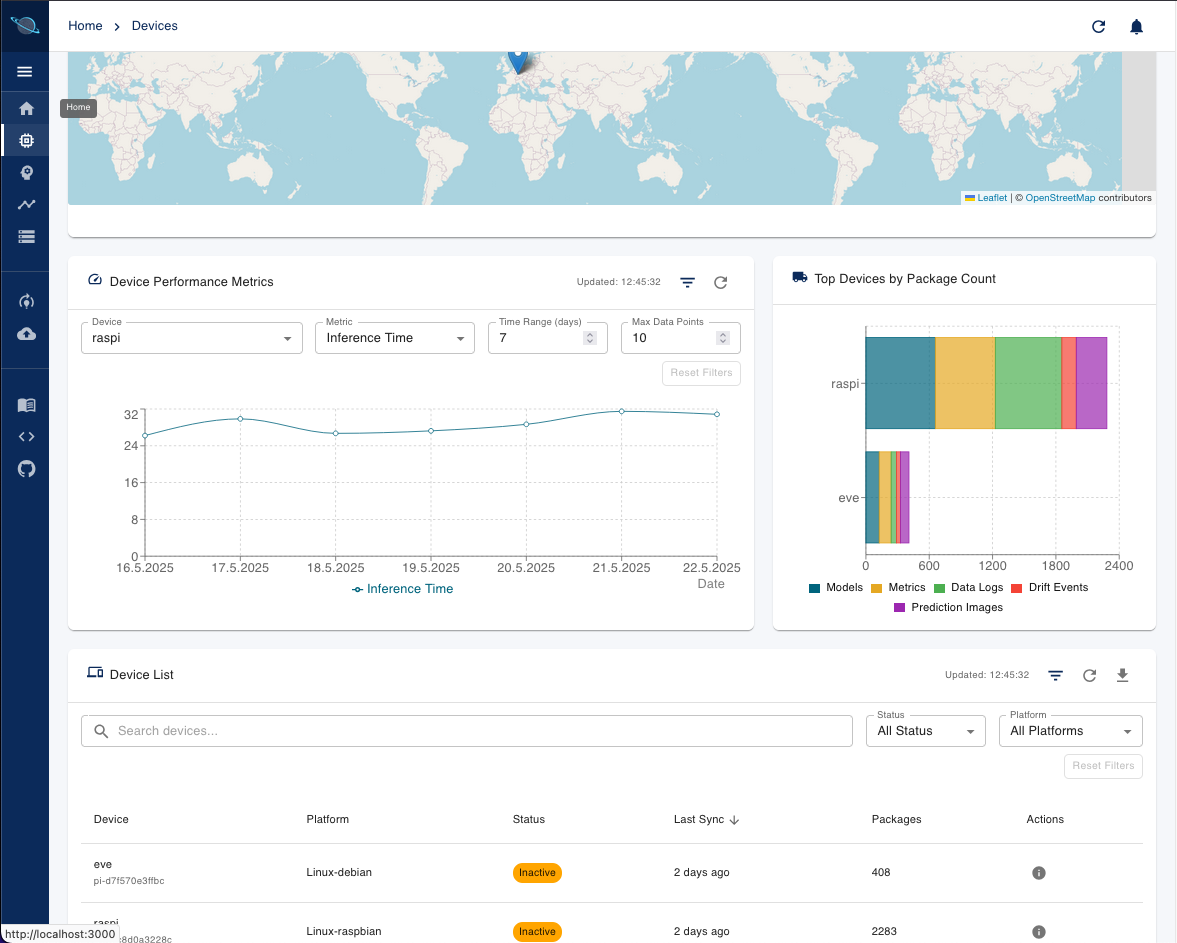
\includegraphics[width=\textwidth]{figs/framework/device-page.png}
        \caption{TinySphere device page providing an overview of the device fleet, including status, key statistics, and location data for individual devices.}
        \label{fig:ui_device_page}
    \end{subfigure}
    \hfill
    \begin{subfigure}[b]{0.48\textwidth}
        \centering
        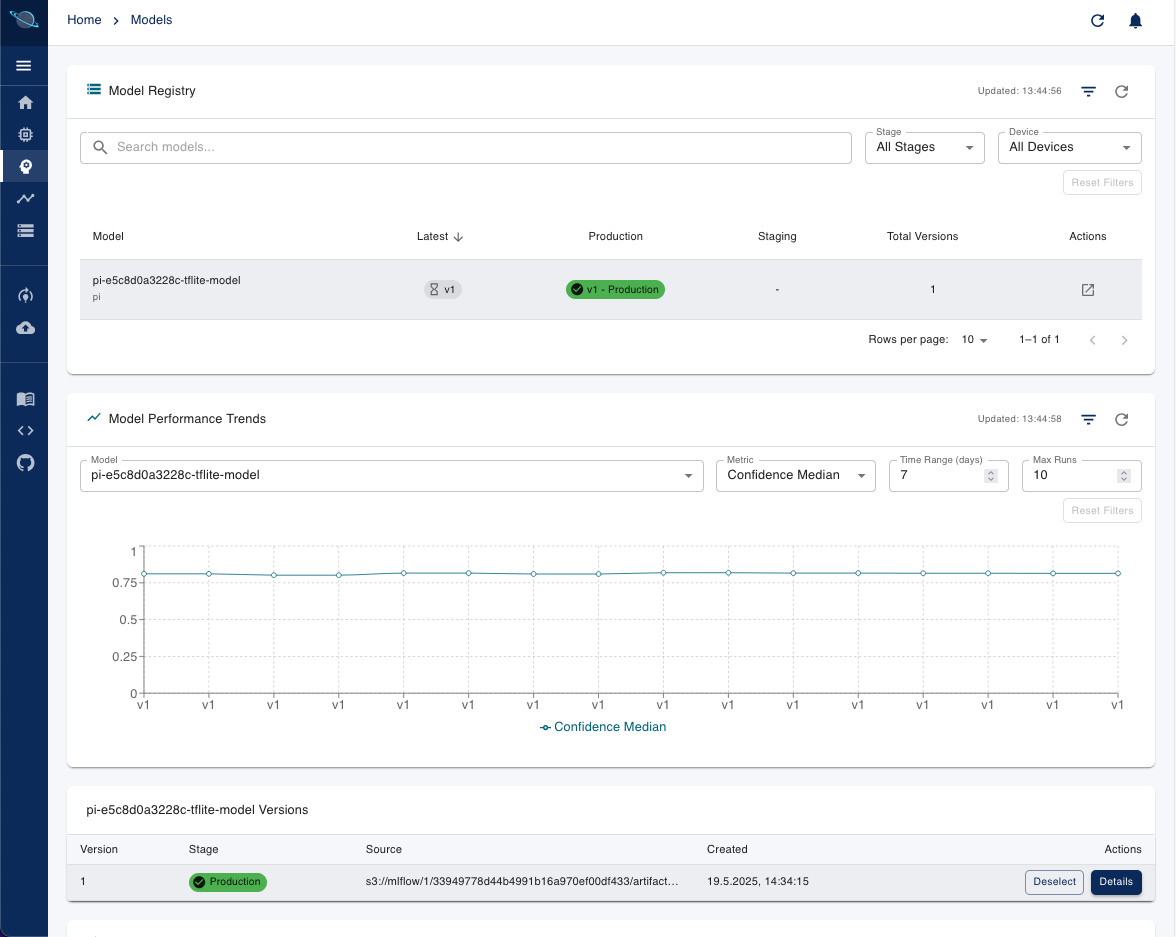
\includegraphics[width=\textwidth]{figs/framework/model-page.png}
        \caption{Model registry interface in TinySphere, listing available \gls{ml} models, their versions, and associated metadata for management.}
        \label{fig:ui_model_registry}
    \end{subfigure}

    \vspace{1em}

    \begin{subfigure}[b]{0.48\textwidth}
        \centering
        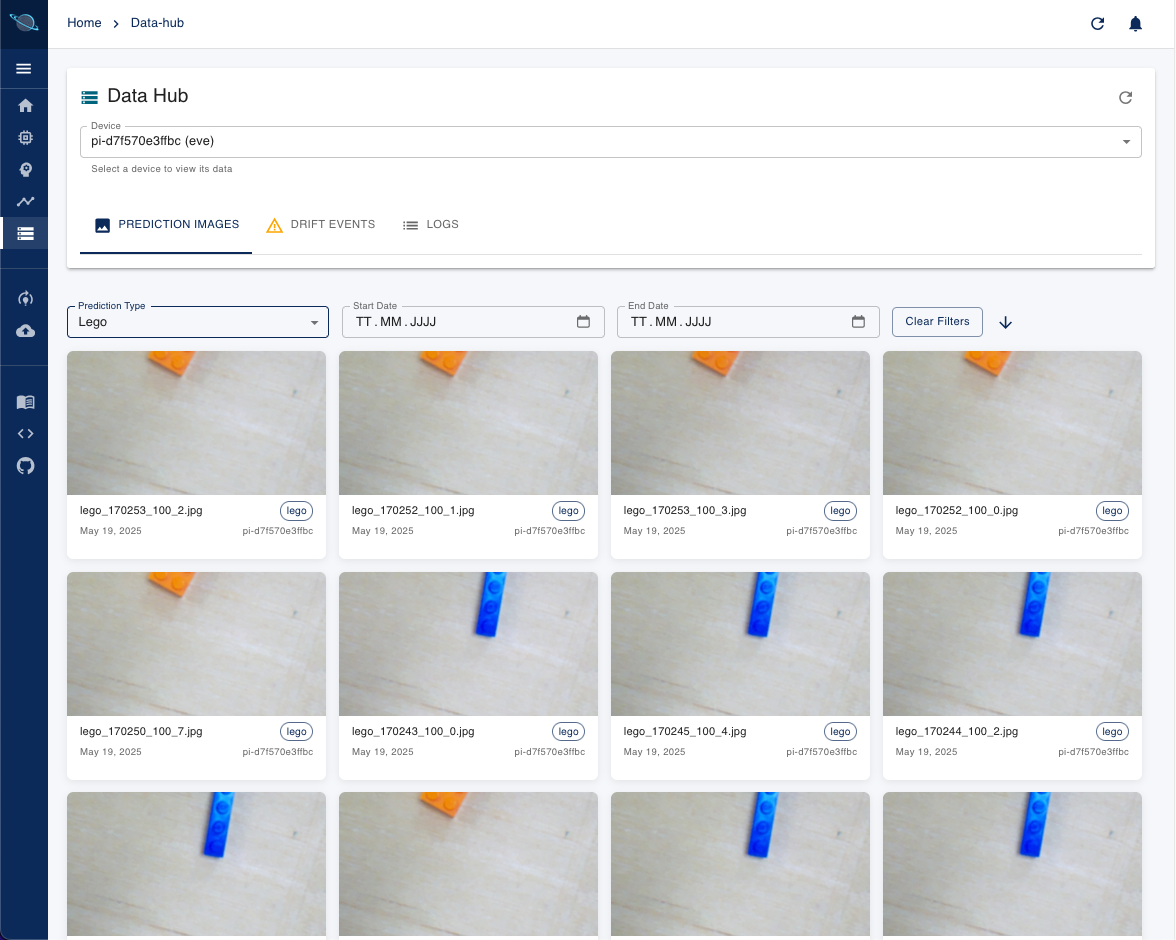
\includegraphics[width=\textwidth]{figs/framework/data-hub-page.png}
        \caption{Data Hub view in TinySphere, illustrating the aggregation and accessibility of data collected from deployed \gls{tinylcm} devices.}
        \label{fig:ui_data_hub}
    \end{subfigure}
    \hfill
    \begin{subfigure}[b]{0.48\textwidth}
        \centering
        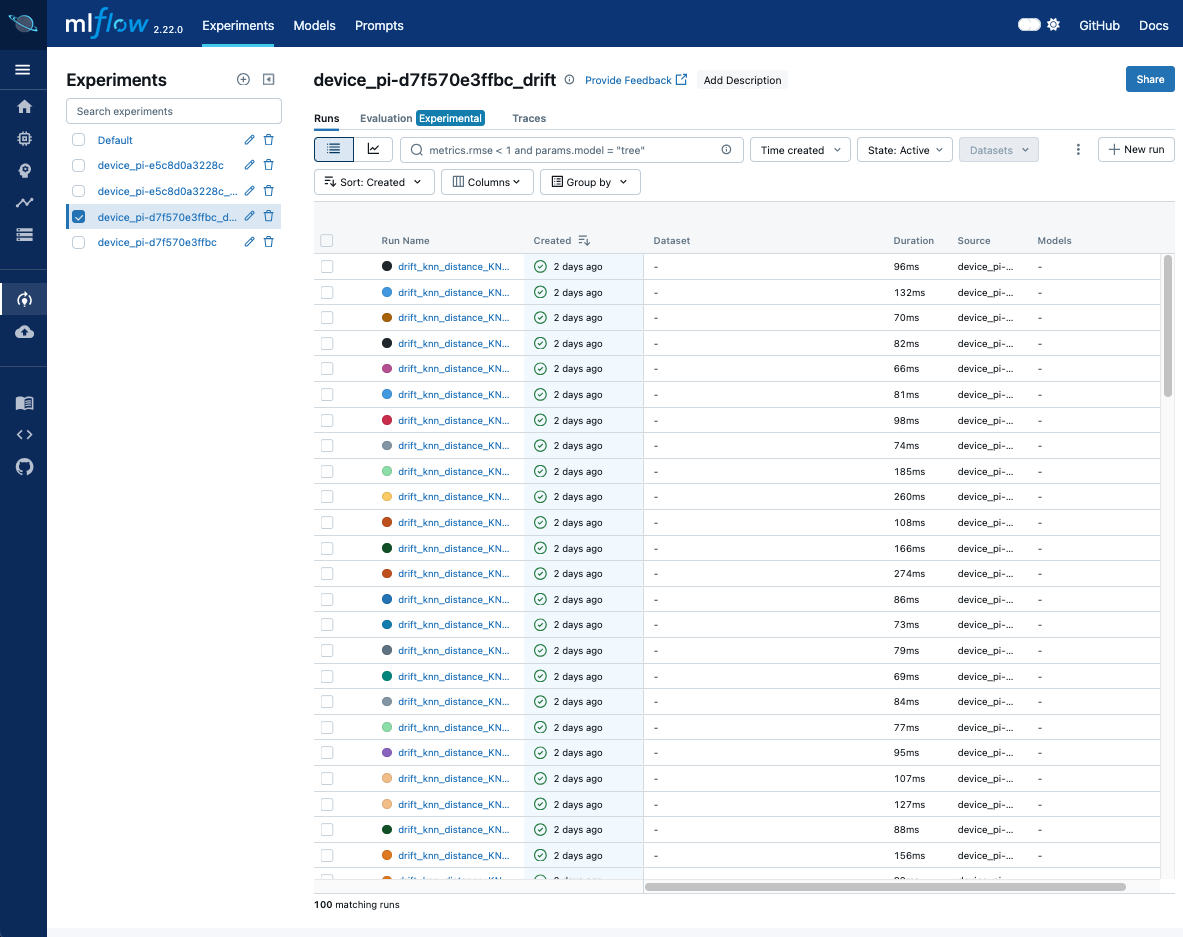
\includegraphics[width=\textwidth]{figs/framework/mlflow-page.png}
        \caption{Integration with MLflow, showcasing tracked experiments and runs, including logged parameters, metrics, and artifacts.}
        \label{fig:ui_mlflow_integration}
    \end{subfigure}

    \vspace{1em}
    \begin{subfigure}[b]{0.48\textwidth}
        \centering
        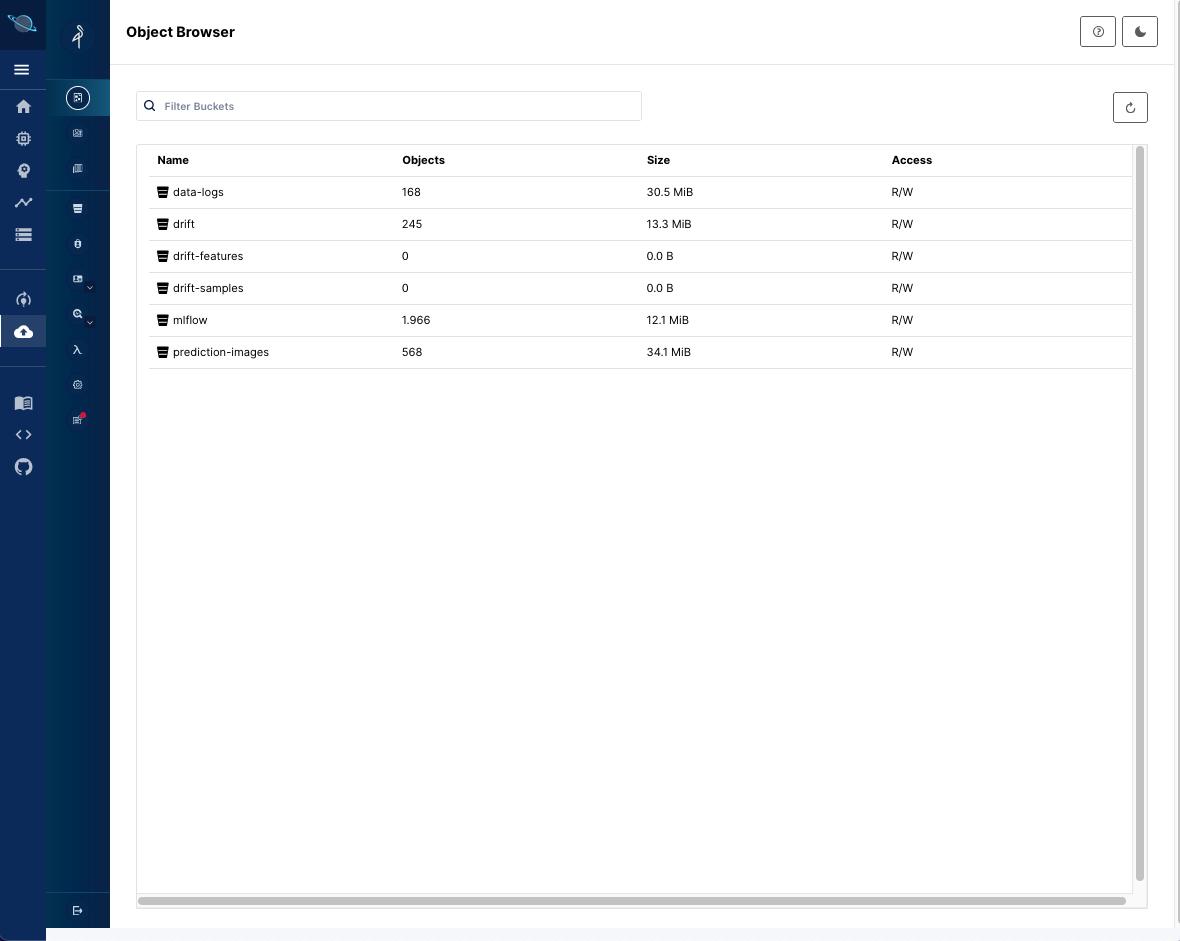
\includegraphics[width=\textwidth]{figs/framework/minio-page.png}
        \caption{MinIO object storage integration, displaying the bucket structure used for storing artifacts such as models, datasets, and logs.}
        \label{fig:ui_minio_integration}
    \end{subfigure}
    \hfill
    \begin{subfigure}[b]{0.48\textwidth}
        \centering
        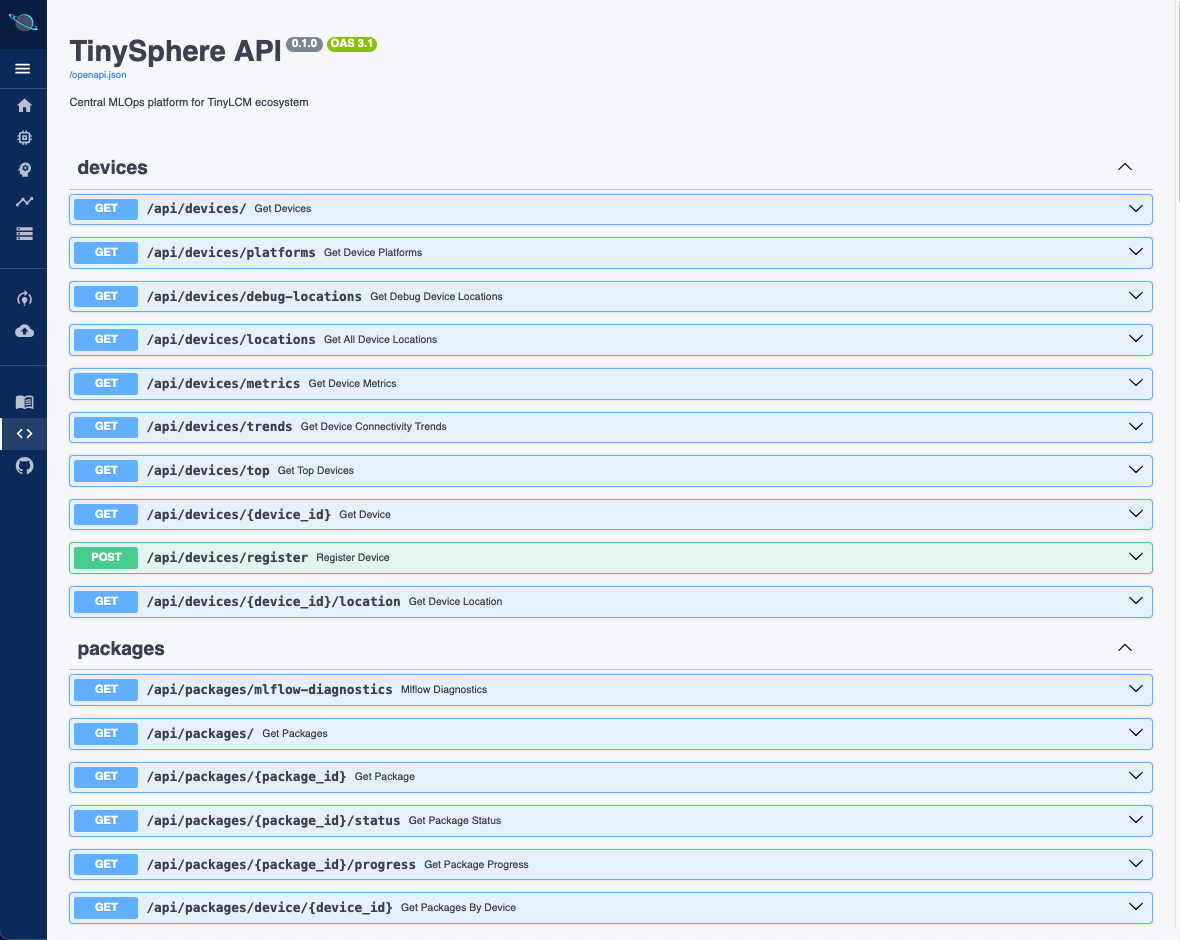
\includegraphics[width=\textwidth]{figs/framework/api-page.png}
        \caption{Integrated OpenAPI (Swagger) documentation for the TinySphere API, providing an interactive reference for developers.}
        \label{fig:ui_openapi_docs}
    \end{subfigure}

    \caption[Illustrative mockups of TinySphere User Interface components]{Illustrative mockups of TinySphere User Interface components and integrations supporting the MLOps workflow: (a) Device fleet management page, (b) Model registry, (c) Data Hub, (d) MLflow experiment tracking, (e) MinIO bucket structure, and (f) OpenAPI documentation.}
    \label{fig:tinysphere_ui_examples}
\end{figure}

%!TEX root = thesis.tex

\chapter{Evaluation of the Framework}
\label{chp:Evaluation}

This chapter presents the empirical evaluation of the \gls{tinylcm} framework, conducted according to the refined experimental design detailed in Section~\ref{sec:FrameworkEvaluationMethodology}. The evaluation is structured into two primary phases: Phase 1 assesses the performance overhead introduced by \gls{tinylcm} components, and Phase 2 validates the framework's functional drift detection capabilities. The results are analyzed to test the hypotheses H$_1$, H$_2$, and H$_3$ formulated in Section~\ref{ssec:refined_experimental_design_final}. Finally, a cross-phase discussion synthesizes the findings, and potential threats to the validity of these results are considered.

~\\
\vfill
\minitoc
\clearpage

\section{Experimental Setup Implementation}
\label{sec:exper-setup_implementation}

The experiments were conducted in a controlled laboratory environment to ensure consistency and reproducibility, as described in Section~\ref{ssec:refined_experimental_design_final}. Figure~\ref{fig:exp_setup_photo} illustrates the physical setup used for data collection. Key aspects included fixed camera positioning (\SI{15}{\centi\meter} to object surface), defined object placement markers, and controlled lighting conditions (dual artificial light sources, minimized ambient light) to reduce environmental variability.

\begin{figure}[htbp]
  \centering
  \includegraphics[width=.55\linewidth]{figs/evaluation/exp_setup.png}
  \caption[Photograph of the Controlled Experimental Setup]{Physical setup for the controlled experiments, showing the Raspberry Pi Zero 2W with camera module, consistent object placement area with markers, and controlled lighting.}
  \label{fig:exp_setup_photo}
\end{figure}

\section{Phase 1 – Performance Overhead Assessment}
\label{sec:phase1_results_overhead}

This phase aimed to quantify the computational and memory overhead introduced by the \gls{tinylcm} framework components. The three staged configurations (Baseline, \gls{tinylcm} (no drift), \gls{tinylcm} (with drift detection)) were executed in five independent runs each. After excluding the warm-up period, a substantial number of measurements ($N$) were collected for each configuration.


\subsection{Resource Utilization and Inference Latency}
\label{ssec:phase1_combined_analysis_latency}

Table~\ref{tab:performance_summary_values_eval} provides a summary of the key performance metrics. It shows the descriptive statistics (mean and standard deviation) calculated across all individual measurements collected from the five independent runs for each configuration. For a more detailed temporal view, time series visualizations of the CPU, memory, and latency data for each configuration are available in Appendix~\ref{app:eval-data}.

\begin{table}[htbp]
    \centering
    \caption[Descriptive Statistics of Performance Metrics from All Measurements (Phase 1)]{Descriptive statistics for key performance metrics, calculated over all measurements ($N$) from the five independent runs.}
    \label{tab:performance_summary_values_eval}
    \footnotesize
    \begin{tabularx}{\linewidth}{@{}X c r@{$\pm$}l r@{$\pm$}l r@{$\pm$}l@{}}
        \toprule
        \textbf{Configuration} & \textbf{$N$} & \multicolumn{2}{c}{CPU Usage (\%)} & \multicolumn{2}{c}{Memory (MB)} & \multicolumn{2}{c}{Latency (ms)} \\
        \midrule
        Baseline \gls{tfl} & 1306 & 3.33 & 1.73 & 174.55 & 0.24 & 357.68 & 1.91 \\
        \gls{tinylcm} (no drift) & 1089 & 5.39 & 3.03 & 229.93 & 1.65 & 419.66 & 4.36 \\
        \gls{tinylcm} (drift detection) & 873 & 4.10 & 3.10 & 203.92 & 9.58 & 435.60 & 43.74 \\
        \bottomrule
    \end{tabularx}
\end{table}

Observing Table~\ref{tab:performance_summary_values_eval} and the corresponding visualizations:
\begin{itemize}[noitemsep, topsep=0pt]
    \item \textit{CPU Usage:} The Baseline configuration showed a mean CPU usage of $3.33 \pm 1.73$\%. This increased to $5.39 \pm 3.03$\% for the \gls{tinylcm} (no drift) configuration. With drift detection enabled, the mean CPU usage was $4.10 \pm 3.10$\%.
    \item \textit{Memory Usage:} Memory usage increased from a mean of $174.55 \pm 0.24$\,\si{\mega\byte} for the Baseline to $229.93 \pm 1.65$\,\si{\mega\byte} for \gls{tinylcm} (no drift). The \gls{tinylcm} (drift detection) configuration had a mean memory of $203.92 \pm 9.58$\,\si{\mega\byte}.
    \item \textit{Inference Latency:} Mean inference latency increased from $357.68 \pm 1.91$\,\si{\milli\second} for the Baseline to $419.66 \pm 4.36$\,\si{\milli\second} for \gls{tinylcm} (no drift), and further to $435.60 \pm 43.74$\,\si{\milli\second} for the full framework. The significantly larger standard deviation for the drift detection configuration suggests the presence of high-latency outliers, likely corresponding to the execution of the drift check itself.
\end{itemize}

While Table~\ref{tab:performance_summary_values_eval} provides a global overview of all collected data points, the subsequent hypothesis testing relies on treating each of the five experimental runs as an independent sample. This approach is methodologically crucial to avoid pseudo-replication and to validly assess the variability between runs. Therefore, the statistical tests in Section~\ref{ssec:phase1_hyp_tests} are performed on the distributions of the $n=5$ aggregate values. The distributions of these aggregate values are visualized through boxplots in Figure~\ref{fig:performance_boxplots_eval} and histograms in Figure~\ref{fig:performance_histograms_density_eval}.

\begin{figure}[htbp]
  \centering
  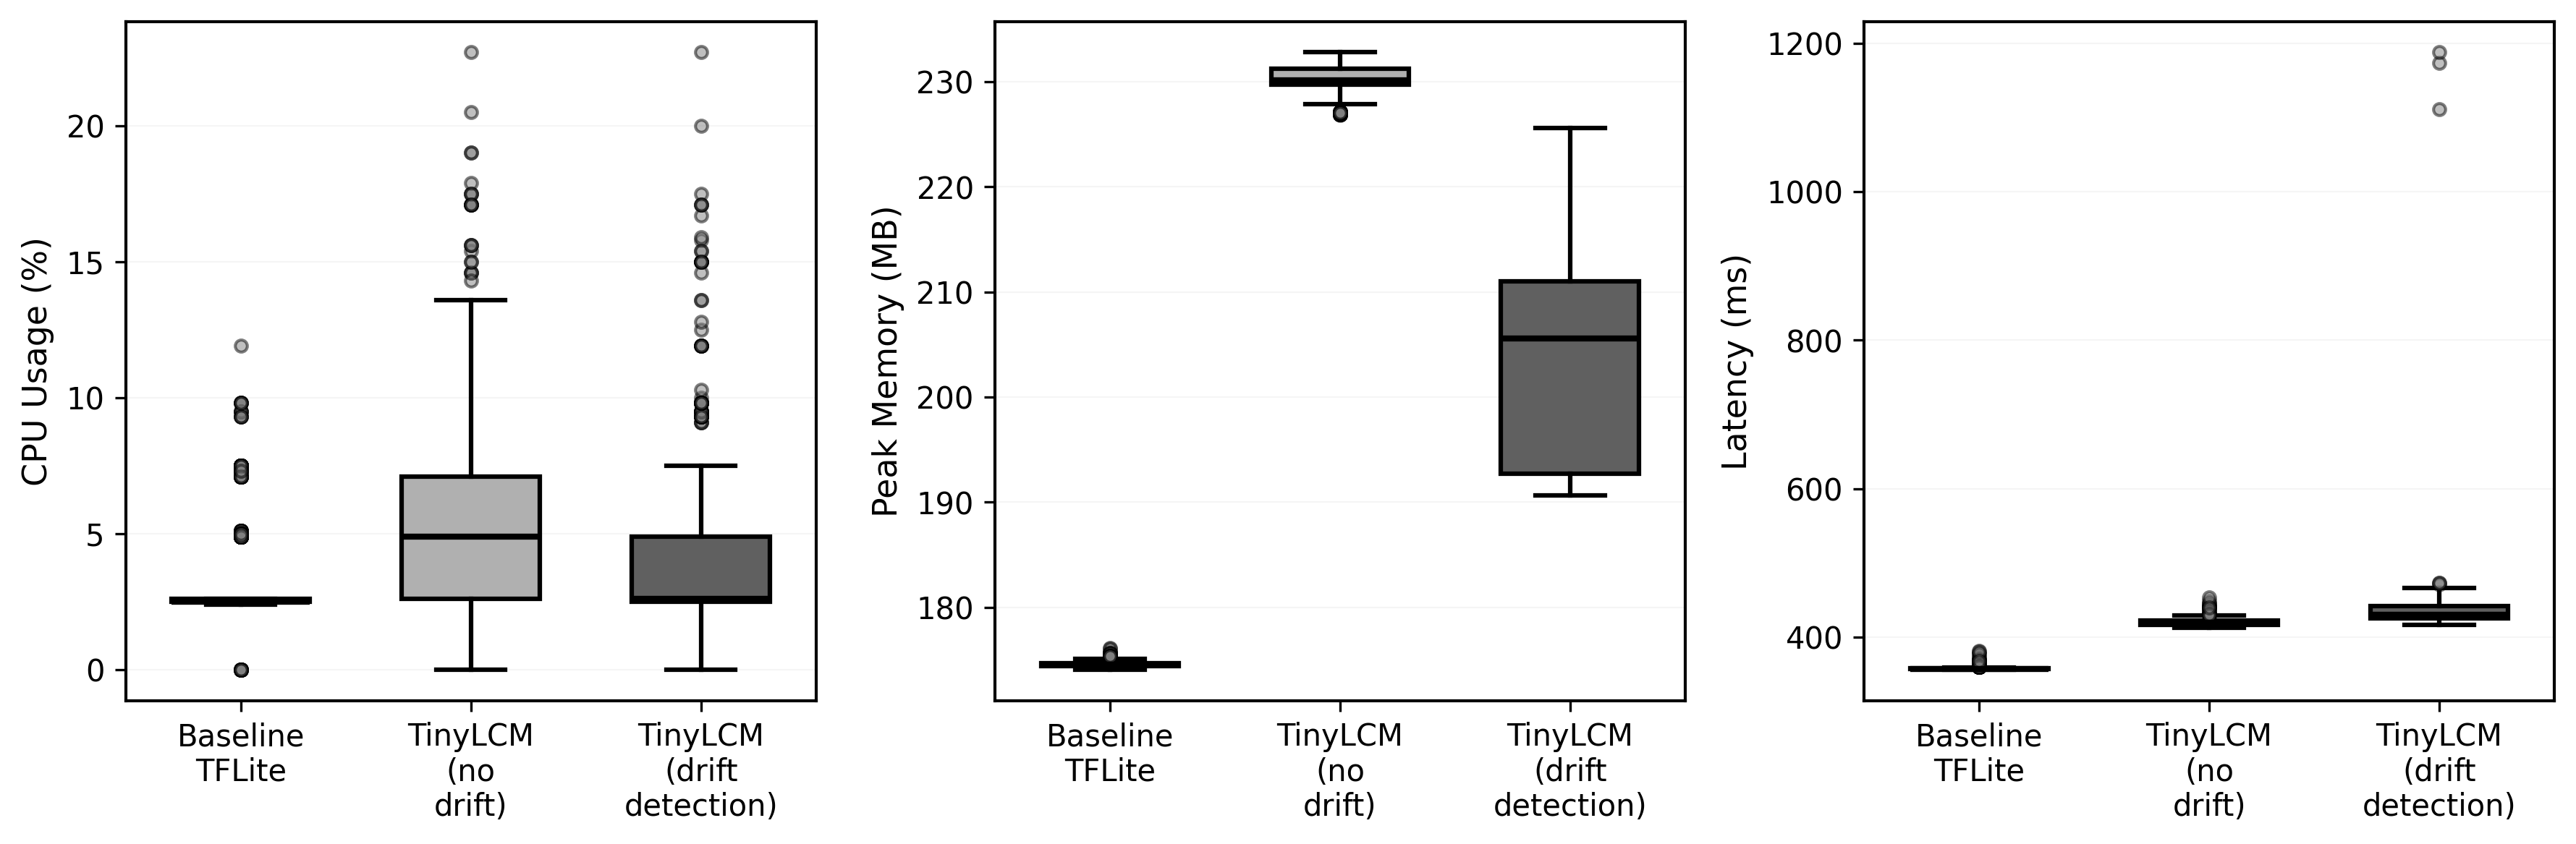
\includegraphics[width=.98\linewidth]{figs/evaluation/boxplots_N5.png}
  \caption[Boxplot Analysis of Aggregated Performance Metrics]{Comparative boxplot analysis of CPU usage (\%), memory (\si{\mega\byte}), and latency (\si{\milli\second}) for the three configurations, based on the runs per configuration. Individual data points are overlaid.}
  \label{fig:performance_boxplots_eval}
\end{figure}

\begin{figure}[htbp]
  \centering
  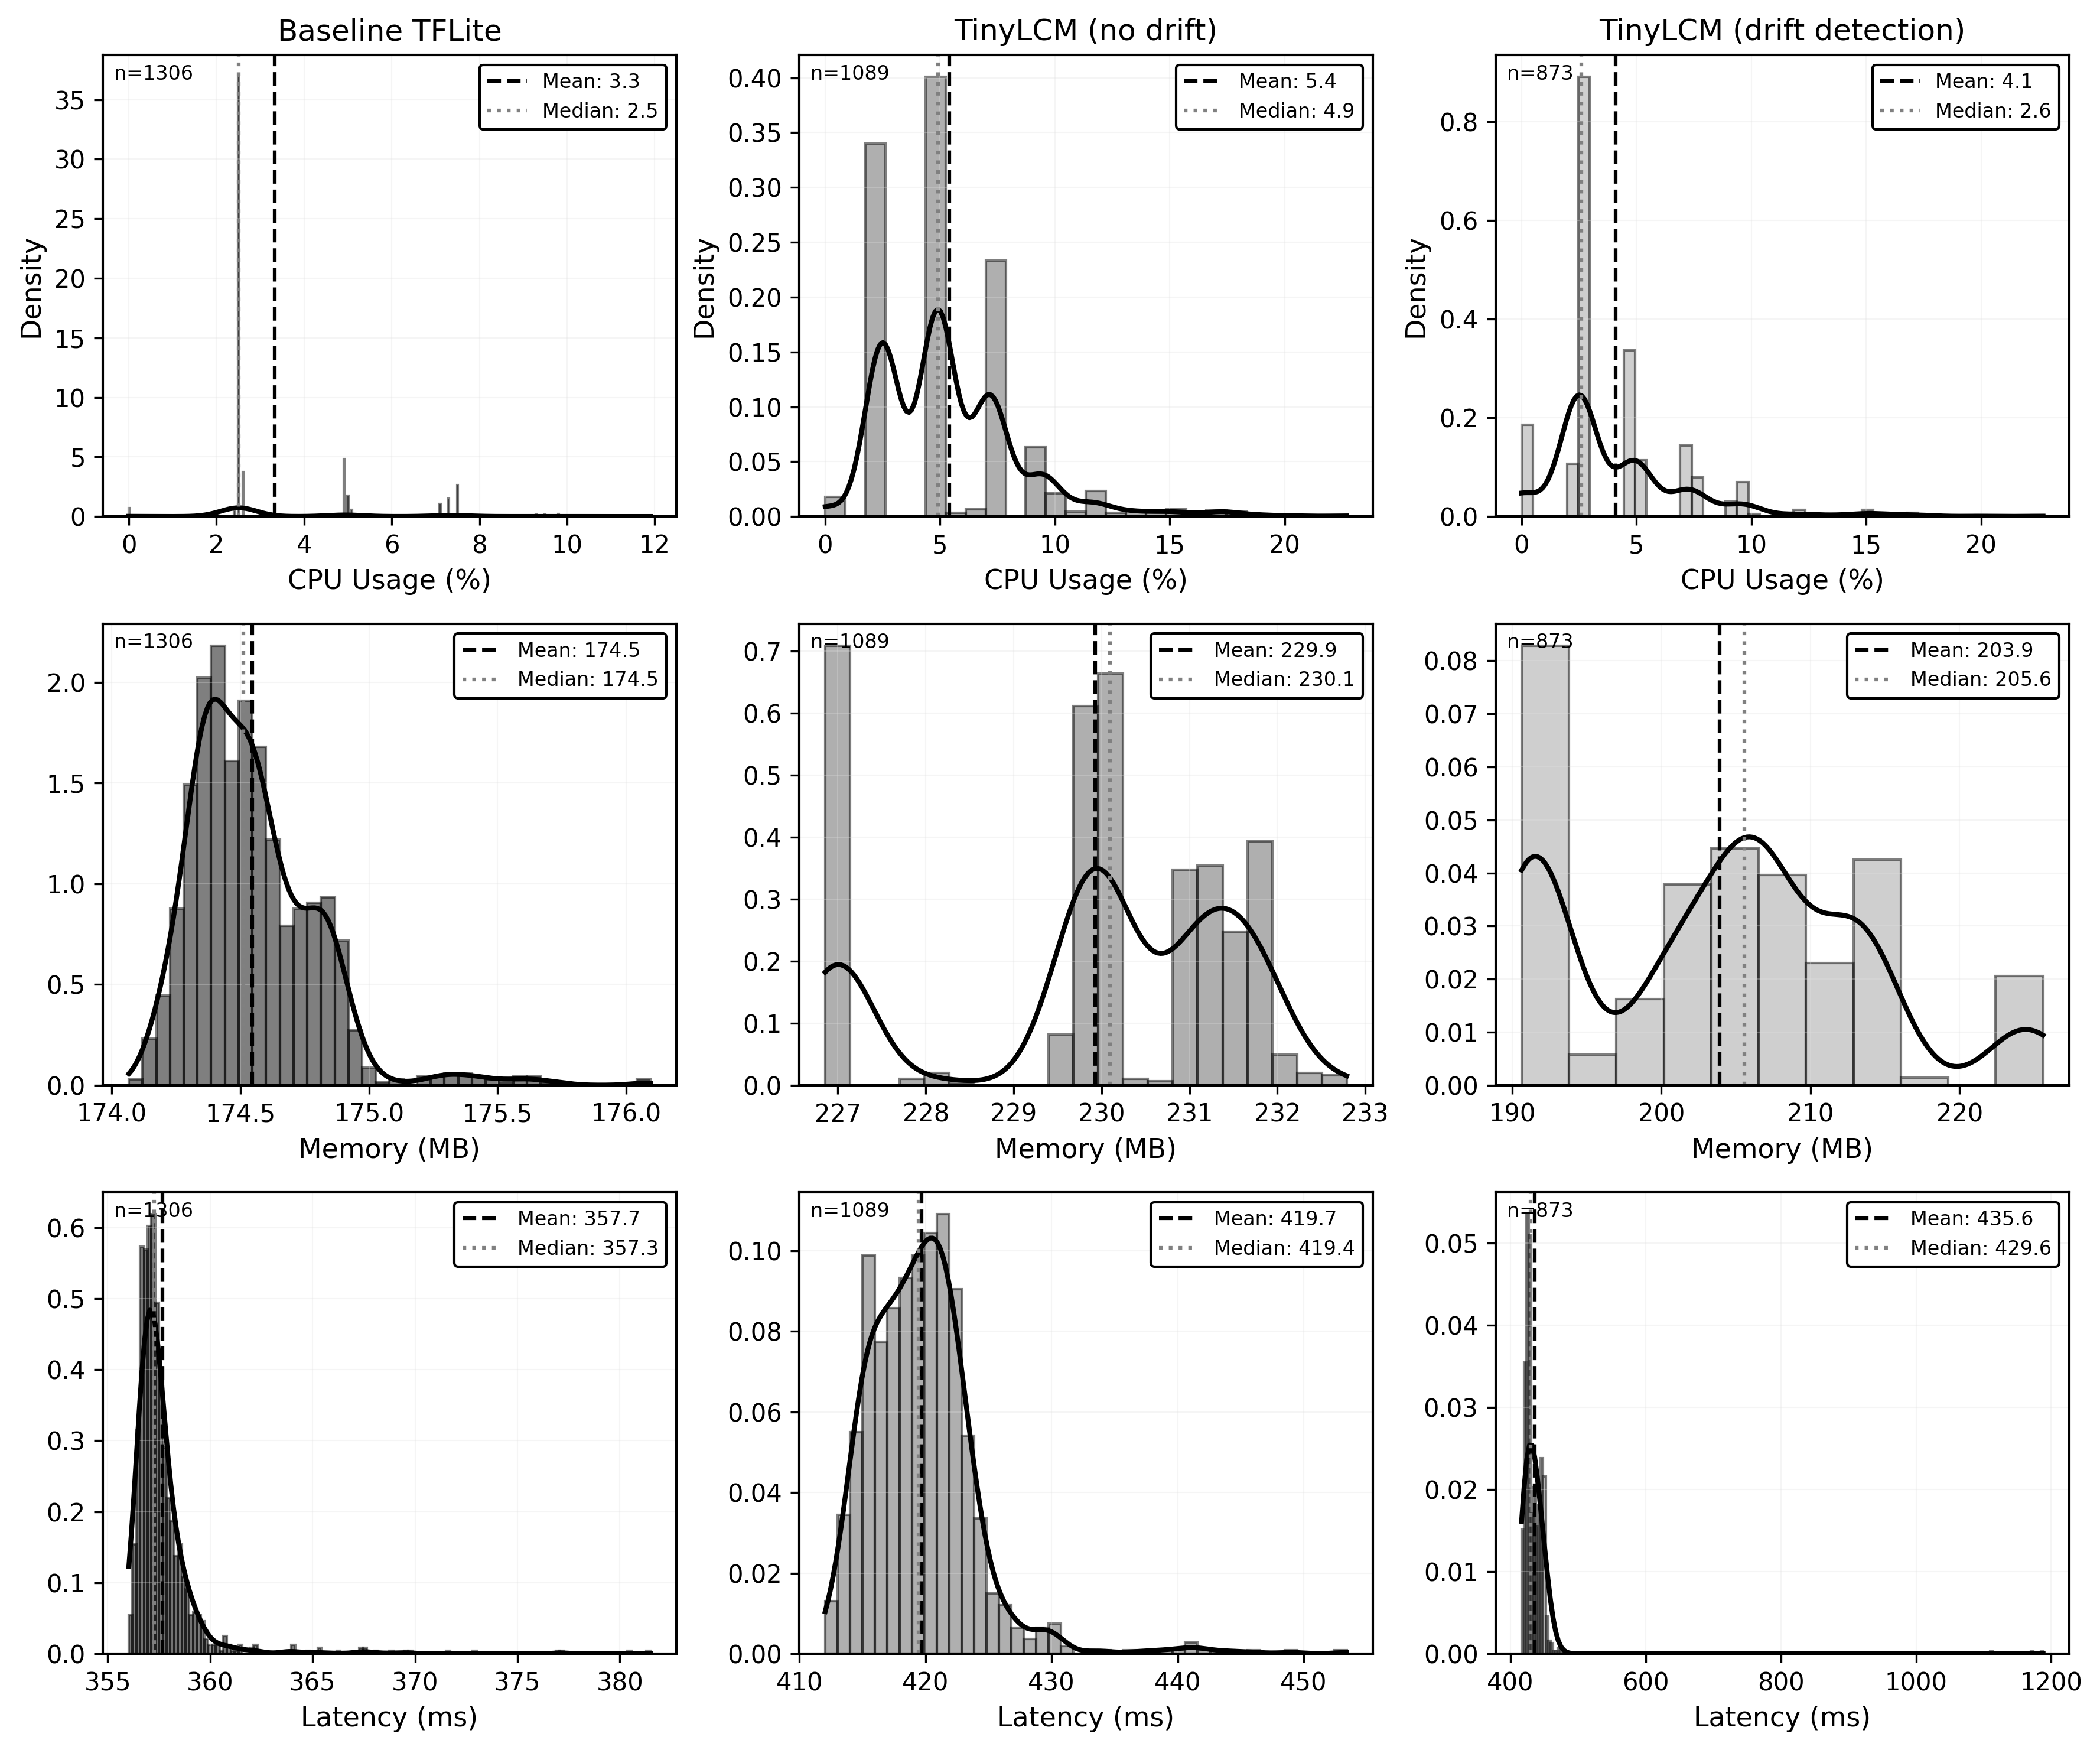
\includegraphics[width=.98\linewidth]{figs/evaluation/histograms_density_N5.png}
  \caption[Histograms and Kernel Density Estimates of Aggregated Performance Metrics]{Distributions of CPU usage (\%), memory (\si{\mega\byte}), and latency (\si{\milli\second}) for the three configurations, based on the runs per configuration. Histograms are overlaid with kernel density estimates and a vertical line indicating the mean.}
  \label{fig:performance_histograms_density_eval}
\end{figure}

\subsection{Hypothesis Testing (H$_1$ and H$_2$)}
\label{ssec:phase1_hyp_tests}

Prior to hypothesis testing, the full datasets for each metric and configuration (N > 800) were assessed for normality using the Shapiro-Wilk test. The tests confirmed that all examined distributions significantly deviate from normality (all $p \ll 0.001$). Consequently, non-parametric one-sample Wilcoxon signed-rank tests were used to evaluate H$_1$ and H$_2$ against their defined thresholds. The results are summarized in Table~\ref{tab:h1_h2_test_results}.

As shown in Table~\ref{tab:h1_h2_test_results}, all tests yielded highly significant results ($p \ll 0.001$), confirming that the observed performance metrics are well within their predefined acceptable limits. The latency overhead for both \gls{tinylcm} configurations was significantly below 50\%. Likewise, the CPU and memory usage were significantly below their respective thresholds. Therefore, both \textbf{H$_1$ and H$_2$ are accepted}.

\begin{table}[htbp]
    \centering
    \caption[Summary of Hypothesis Test Results for H$_1$ and H$_2$]{Results of the one-sided one-sample Wilcoxon signed-rank tests for H$_1$ and H$_2$.}
    \label{tab:h1_h2_test_results}
    \footnotesize
    \begin{tabularx}{\linewidth}{@{}l l X r c r@{}}
        \toprule
        \textbf{Hypothesis} & \textbf{Metric} & \textbf{Configuration} & \textbf{Statistic (W)} & \textbf{Threshold} & \textbf{$p$-value} \\
        \midrule
        \textbf{H$_1$} & Latency Overhead & \gls{tinylcm} (no drift) & 0.0 & < 50\% & $5.10\times10^{-180}$ \\
                      &                   & \gls{tinylcm} (drift detection) & 2616.0 & < 50\% & $6.53\times10^{-141}$ \\
        \addlinespace
        \textbf{H$_2$} & CPU Usage & \gls{tinylcm} (no drift) & 0.0 & < 50\% & $2.17\times10^{-180}$ \\
                      &           & \gls{tinylcm} (drift detection) & 0.0 & < 50\% & $1.44\times10^{-146}$ \\
        \addlinespace
        \textbf{H$_2$} & Memory & \gls{tinylcm} (no drift) & 0.0 & < 256 MB & $5.10\times10^{-180}$ \\
                      &        & \gls{tinylcm} (drift detection) & 0.0 & < 256 MB & $8.57\times10^{-145}$ \\
        \bottomrule
    \end{tabularx}
\end{table}

To compare the performance between configurations, the Mann-Whitney U test was used, with Cliff's delta ($\delta$) as the measure of effect size. The results are summarized in Table~\ref{tab:phase1_mannwhitney_results}. It demonstrate that all pairwise comparisons between the configurations yielded statistically significant differences. The addition of the \gls{tinylcm} pipeline (S1) to the baseline (S0) resulted in a medium increase in CPU usage and a large increase in memory and latency. Adding drift detection (S2) also caused a significant increase in latency and memory compared to baseline, though the effect on CPU usage was negligible.
Comparing the two \gls{tinylcm} configurations directly, the full framework with drift detection (S2) exhibited significantly higher latency (large effect) but significantly lower CPU usage (small effect) and memory usage (large effect) than the pipeline without drift detection (S1). This counterintuitive result regarding CPU and memory is further explored in the methodological reflection below.

\begin{table}[htbp]
  \centering
  \caption[Mann-Whitney U Test Results for Phase 1 Performance Metrics]{Mann-Whitney U test results and Cliff's delta effect sizes for comparing independent configurations. S1 = \gls{tinylcm} (no drift), S2 = \gls{tinylcm} (with drift detection), S0 = Baseline. Effect size interpretation: L=Large, M=Medium, S=Small, N=Negligible.}
  \label{tab:phase1_mannwhitney_results}
  \footnotesize
  \setlength{\tabcolsep}{3pt} 
  \begin{tabularx}{\linewidth}{@{}X r c r@{}} 
    \toprule
    \textbf{Metric (Comparison Pair)} & \textbf{Statistic ($U$)} & \textbf{$p$-value} & \textbf{Cliff's $\delta$ (Interpretation)} \\ 
    \midrule
    CPU Usage (\%) (S1 vs. S0)      & $997726.5$ & $4.25\times10^{-70}$ & $+0.40$ (M) \\
    CPU Usage (\%) (S2 vs. S0)      & $636664.0$ & $4.09\times10^{-7}$ & $+0.12$ (N) \\ 
    CPU Usage (\%) (S2 vs. S1)      & $353119.0$ & $5.16\times10^{-23}$ & $-0.26$ (S) \\ 
    \addlinespace
    Memory (\si{\mega\byte}) (S1 vs. S0)    & $1422234.0$ & $0.0$ & $+1.0$ (L) \\ 
    Memory (\si{\mega\byte}) (S2 vs. S0)    & $1140138.0$ & $0.0$ & $+1.0$ (L) \\
    Memory (\si{\mega\byte}) (S2 vs. S1)    & $0.0$       & $0.0$ & $-1.0$ (L) \\
    \addlinespace
    Latency (\si{\milli\second}) (S1 vs. S0)   & $1422234.0$ & $0.0$ & $+1.0$ (L) \\
    Latency (\si{\milli\second}) (S2 vs. S0)   & $1140138.0$ & $0.0$ & $+1.0$ (L) \\
    Latency (\si{\milli\second}) (S2 vs. S1)   & $877097.0$  & $1.08\times10^{-227}$ & $+0.85$ (L) \\
    \bottomrule
  \end{tabularx}
\end{table}

\begin{MyBox}{Methodological Reflection on Experimental Run Order and Observed Variances}
    During the execution of the Phase 1 performance experiments, an observation was made regarding resource utilization that warrants reflection. As indicated in Table~\ref{tab:performance_summary_values_eval} and confirmed by the statistical tests in Table~\ref{tab:phase1_mannwhitney_results}, the \gls{tinylcm} (no drift) configuration (S1) exhibited significantly higher memory ($229.93$\,\si{\mega\byte}) and CPU usage ($5.39\%$) compared to the \gls{tinylcm} (with drift detection) configuration (S2) (memory: $203.92$\,\si{\mega\byte}, CPU: $4.10\%$). This is counterintuitive, as S2 performs strictly more operations than S1.

    While the Python code for both configurations is functionally correct, this specific pattern might be partly attributable to the experimental execution history. The $n=5$ runs for each configuration block (Baseline, S1, S2) were performed as distinct sets, with system restarts intended between the blocks. However, it was noted that the S1 runs were conducted at an earlier stage of the overall experimental campaign, possibly involving more iterative adjustments in the setup or more intensive system activity immediately preceding or during some of those runs compared to the later S2 runs. Such historical factors, even with restarts, could potentially lead to subtle differences in the system's baseline state (e.g., OS caching, background process activity accumulated over time, or even minor variations in ambient temperature affecting the hardware) that might influence resource measurements, especially for memory and CPU.

    Ideally, to completely mitigate such potential temporal or historical biases, a more rigorous protocol would involve a fully randomized or counterbalanced execution order of the three configurations across the 5 ``runs'' (where each run contains one instance of each configuration), along with complete system state resets (e.g., reflashing the OS) before each run.
    
    This reflection does not invalidate the primary findings regarding the overall overhead compared to baseline or the feasibility within resource constraints (H$_1$, H$_2$). However, it provides important context for interpreting fine-grained differences between the two \gls{tinylcm} configurations and underscores a potential subtle threat to internal validity, further discussed in Section~\ref{sec:result_level_threats_validity}.
\end{MyBox}

\subsection{Latency Breakdown}
\label{ssec:phase1_latency_breakdown}

To understand the contributions of different processing stages to the overall inference latency of the \gls{tinylcm} configurations, a detailed breakdown was performed. Table~\ref{tab:latency_components_summary} presents the mean processing times and their percentage contribution to the total latency for each measured component within the ``TinyLCM (no drift)'' and ``TinyLCM (drift detection)'' pipelines. These statistics are derived from aggregating measurements across all processed frames from the $n=5$ independent runs for each configuration, as detailed in the.

\begin{table}[htbp]
    \centering
    \caption[Mean Processing Time of Latency Components for \gls{tinylcm} Configurations (Phase 1)]{Mean processing time and percentage of total latency for each measured component in the \gls{tinylcm} configurations.}
    \label{tab:latency_components_summary}
    \footnotesize
    \begin{tabularx}{\linewidth}{@{}X rr rr@{}} % X für Komponenten, dann 2x rr für Wertepaare
        \toprule
        \textbf{Component} & \multicolumn{2}{c}{\textbf{TinyLCM (no drift)}} & \multicolumn{2}{c}{\textbf{TinyLCM (drift detection)}} \\
        \cmidrule(lr){2-3} \cmidrule(lr){4-5} % Linien unter den Konfigurationsnamen
         & \multicolumn{1}{r}{Mean (\si{\milli\second})} & \multicolumn{1}{r}{(\% Total)} & \multicolumn{1}{r}{Mean (\si{\milli\second})} & \multicolumn{1}{r}{(\% Total)} \\
        \midrule
        Feature Extraction (incl. Base Model, PCA, Scale)$^{\text{a}}$ & 353.71 & 84.29\% & 353.98 & 81.26\% \\
        KNN Inference$^{\text{b}}$ & 65.94 & 15.71\% & 66.42 & 15.25\% \\
        Drift Check & 0.00 & 0.00\% & 1.73 & 0.40\% \\
        Other (Preprocessing, Pipeline Overhead) & 0.01 & 0.00\% & 13.47 & 3.09\% \\
        \midrule
        \textbf{Total Measured Latency} & \textbf{419.66} & \textbf{100\%} & \textbf{435.60} & \textbf{100\%} \\
        \bottomrule
    \end{tabularx}
\end{table}

Table~\ref{tab:latency_components_summary} details the latency contributions. The ``Feature Extraction'' component, which encompasses the execution of the base \gls{tfl} model along with subsequent feature processing steps (such as PCA and scaling), consistently consumes the largest portion of time, averaging approximately $353.71$\,\si{\milli\second} ($84.29\%$) for the ``TinyLCM (no drift)'' configuration and $353.98$\,\si{\milli\second} ($81.26\%$) for the ``TinyLCM (drift detection)'' configuration. This indicates that the core model inference and primary feature derivation dominate the processing time.

The ``KNN Inference'' stage, responsible for the \gls{knn} search and classification based on the processed features, adds a mean of $65.94$\,\si{\milli\second} ($15.71\%$) in the ``no drift'' configuration and $66.42$\,\si{\milli\second} ($15.25\%$) when drift detection is active. The similarity in KNN inference time between the two \gls{tinylcm} configurations is expected, as the core KNN lookup process remains the same.

The ``Drift Check'' component, only active in the ``TinyLCM (drift detection)'' configuration, introduces a mean overhead of $1.73$\,\si{\milli\second}, which constitutes only $0.40\%$ of the total latency for that configuration. This demonstrates that the direct computational cost of the Page-Hinkley test and associated logic for the drift check itself is minimal.

Interestingly, the ``Other (Preprocessing, Pipeline Overhead)'' category shows a notable difference. For the ``TinyLCM (no drift)'' configuration, this overhead is negligible ($0.01$\,\si{\milli\second}). However, for the ``TinyLCM (drift detection)'' configuration, it averages $13.47$\,\si{\milli\second}, accounting for $3.09\%$ of the total latency. This suggests that enabling the drift detection mechanism introduces some additional, unmeasured overhead within the overall pipeline orchestration or data handling steps that occur between the explicitly timed main components. This could include, for example, managing data flow to the drift monitor, conditional checks, or state updates related to the drift detection status, even if the drift check calculation itself is fast. This ``Other'' overhead, when combined with the direct ``Drift Check'' time, largely explains the overall mean latency difference observed between the ``no drift'' ($419.66$\,\si{\milli\second}) and ``drift detection'' ($435.60$\,\si{\milli\second}) configurations as reported in Table~\ref{tab:performance_summary_values_eval}.

\begin{MyBox}{Subjective Interpretation of Latency Results}
	The observed inference latencies, particularly for the \gls{tinylcm} configurations (approx. 420-436\,\si{\milli\second}), correspond to a processing rate of roughly 2.3 frames per second. While acceptable for some near real-time applications, this is relatively high for others demanding faster responses. This latency is influenced by the choice of the MobileNetV2 base model and the Python implementation of \gls{tinylcm}. MobileNetV2 was selected for this study due to its ready availability and straightforward integration after initial attempts with more complex models like EfficientNet Lite encountered compilation and deployment challenges on the target platform. Future work could explore further model optimization or the use of different base architectures to potentially reduce this baseline latency.
\end{MyBox}

\section{Phase 2 – Drift Detection Validation}
\label{sec:phase2_results_drift}

This phase aimed to validate the functional drift detection capabilities of the \gls{tinylcm} framework. The core objective was to test whether the system could produce a statistically significant response to untrained objects. The ground truth for drift periods was determined by analyzing the prediction logs to identify the exact timestamps when untrained objects were presented.

\subsection{Drift Alarm Timelines}
\label{ssec:phase2_alarm_timelines}

Figures~\ref{fig:timeline-exp1_s1} and \ref{fig:timeline-exp2_s2} illustrate the prediction timelines and the occurrences of drift alarms generated by the \texttt{KNNDistanceMonitor} for Scenario 1 and Scenario 2, respectively.

\begin{figure}[htbp]
  \centering
  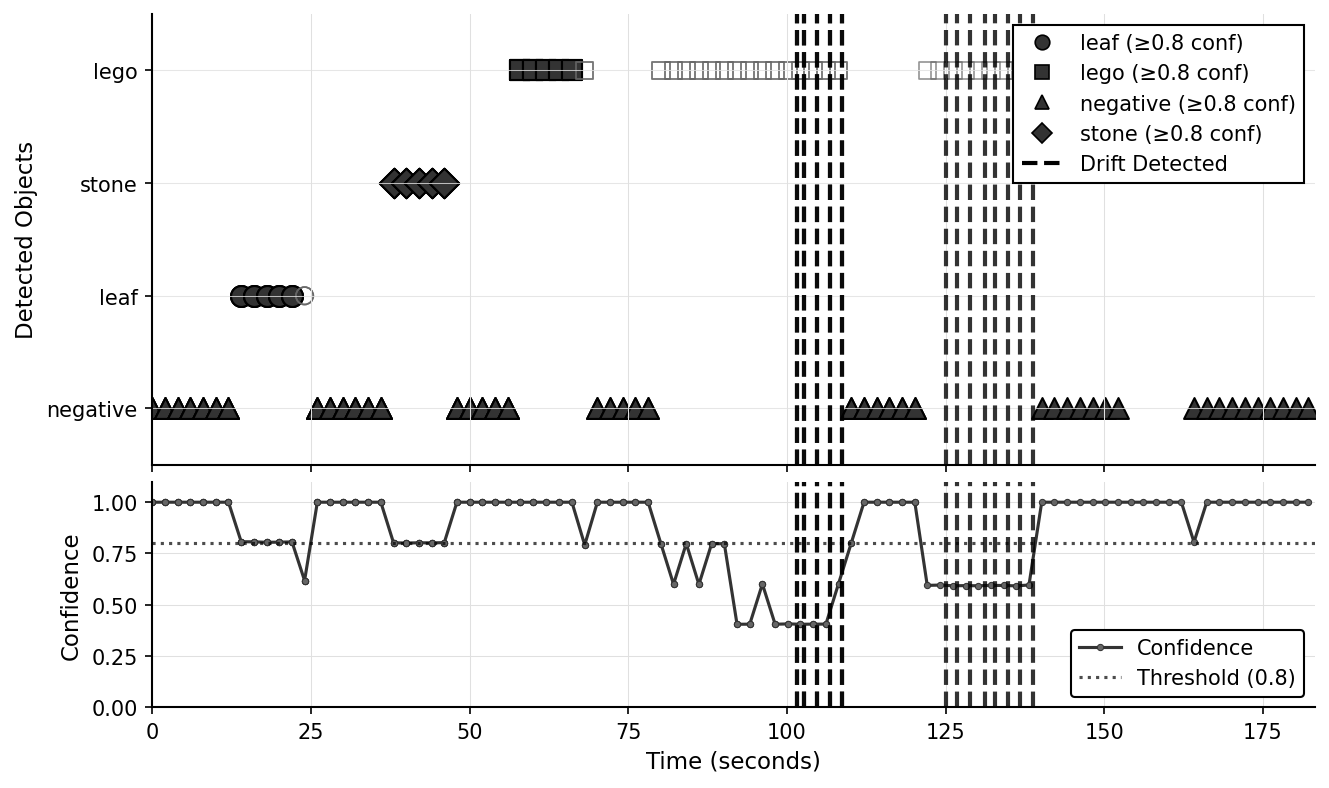
\includegraphics[width=.98\linewidth]{figs/evaluation/drift_coin_ball_timeline.png}
  \caption[Drift Prediction Timeline for Scenario S1 (Dual Drift)]{Prediction timeline and drift alarms for Scenario S1 (Dual Drift). Grey squares indicate the predicted class (y-axis) at each two-second interval. Dashed vertical lines mark drift alarms from the \texttt{KNNDistanceMonitor}. The sequence includes presentation of known classes and two novel drift objects (``ball'', ``coin'').}
  \label{fig:timeline-exp1_s1}
\end{figure}

Following the detection of these drift events, \gls{tinylcm}'s \texttt{SyncClient}, if active and connected, would package relevant information, including images of the objects causing the drift, for transmission to TinySphere. Figures~\ref{fig:drift-image-ball_s1} and \ref{fig:drift-image-coin_s1} show examples of such drift images.

\begin{figure}[htbp]
    \centering
    \begin{subfigure}{0.49\textwidth}
        \centering
        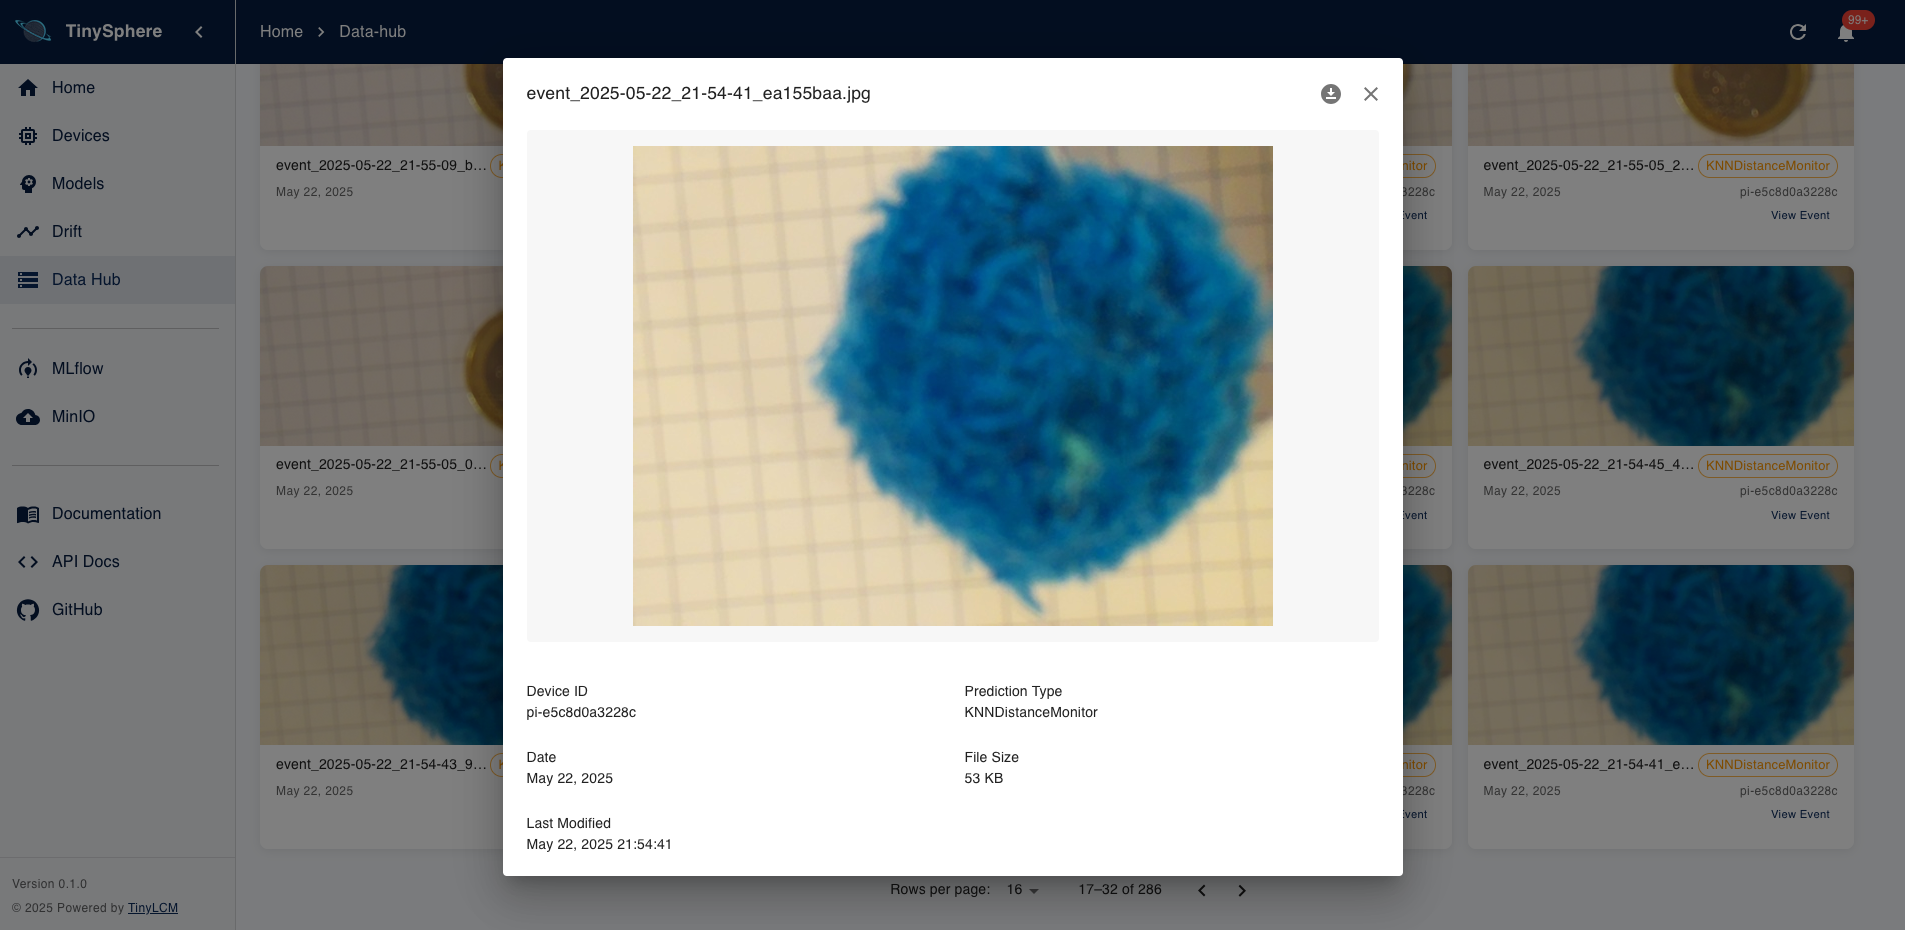
\includegraphics[width=\textwidth]{figs/evaluation/drift_image_exp1_ball.png}
        \caption[Example Drift Image of ``Ball'' (S1)]{Example of a drift-flagged image (object: ``ball'') from  S1, as potentially transmitted to and displayed in the TinySphere Data Hub.}
        \label{fig:drift-image-ball_s1}
    \end{subfigure}
    \hfill 
    \begin{subfigure}{0.49\textwidth}
        \centering
        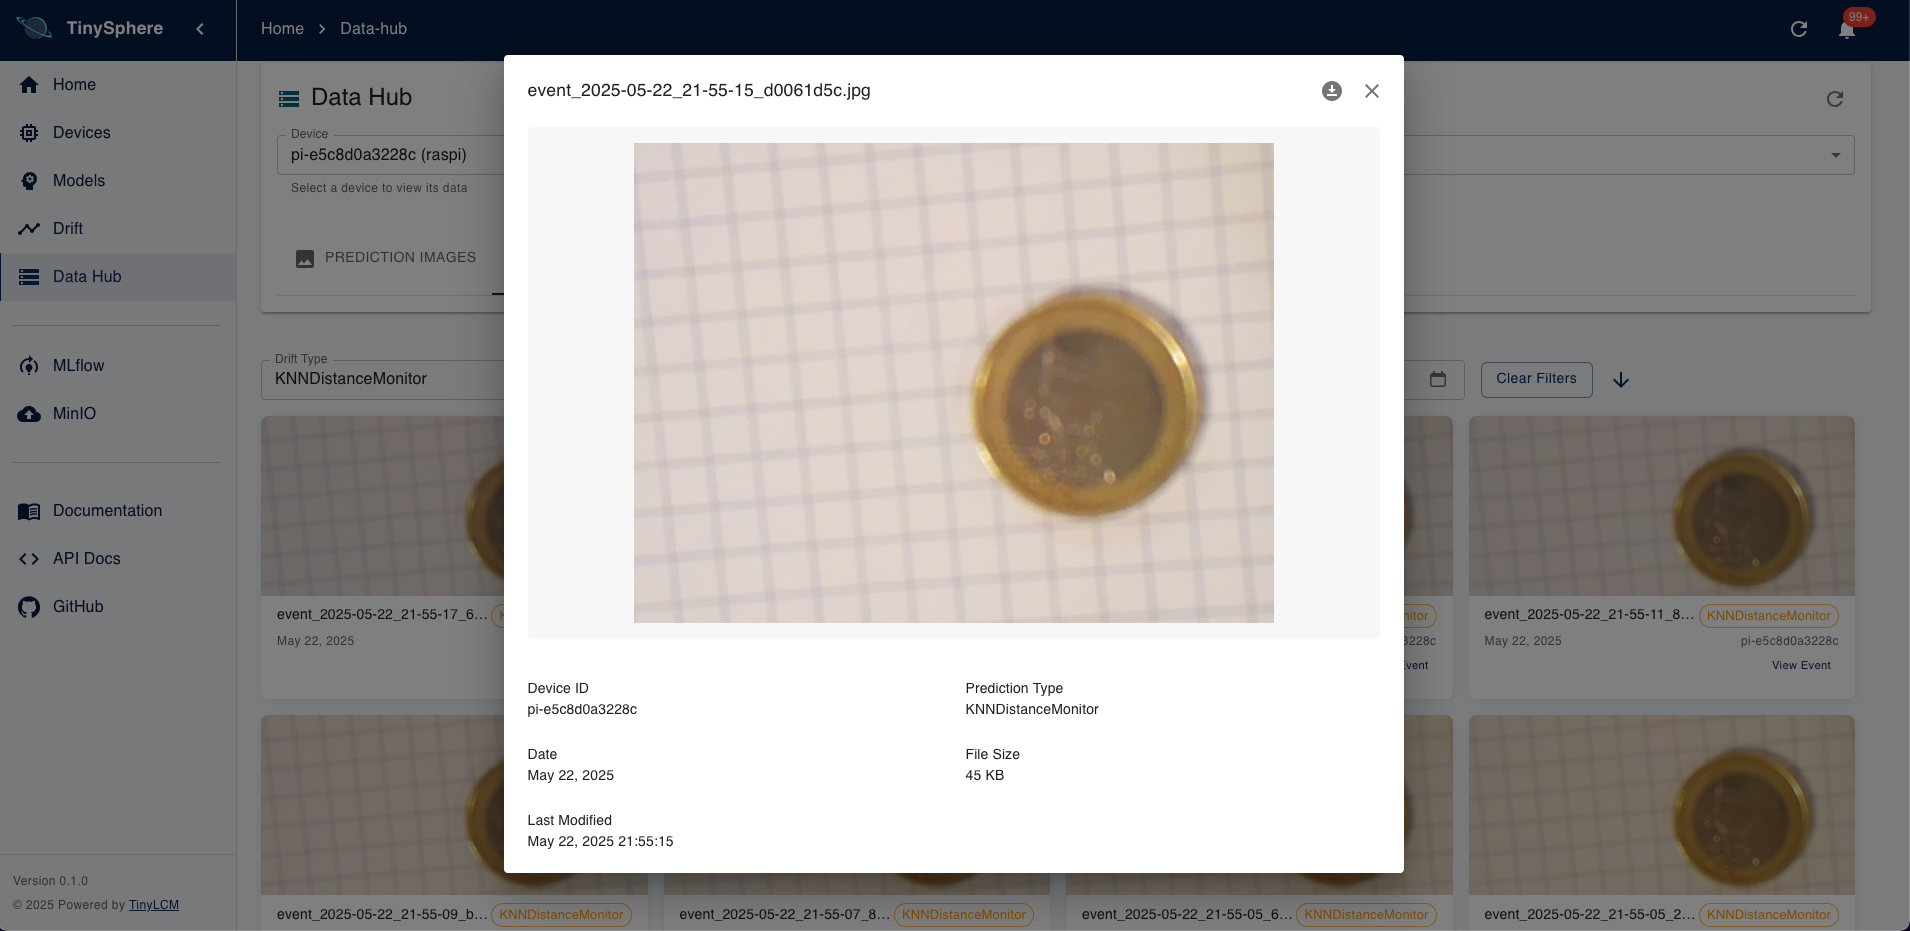
\includegraphics[width=\textwidth]{figs/evaluation/drift_image_exp1_coin.png}
        \caption[Example Drift Image of ``Coin'' (S1)]{Example of a drift-flagged image (object: ``coin'') from  S1, as potentially transmitted to and displayed in the TinySphere Data Hub.}
        \label{fig:drift-image-coin_s1}
    \end{subfigure}
    \caption[Drift Images from S1 (Dual Drift)]{Examples of Drift Images from S1 (Dual Drift) Captured by \gls{tinylcm} and Viewable in TinySphere.}
    \label{fig:combined-drift-images-s1}
\end{figure}

\begin{figure}[htbp]
  \centering
  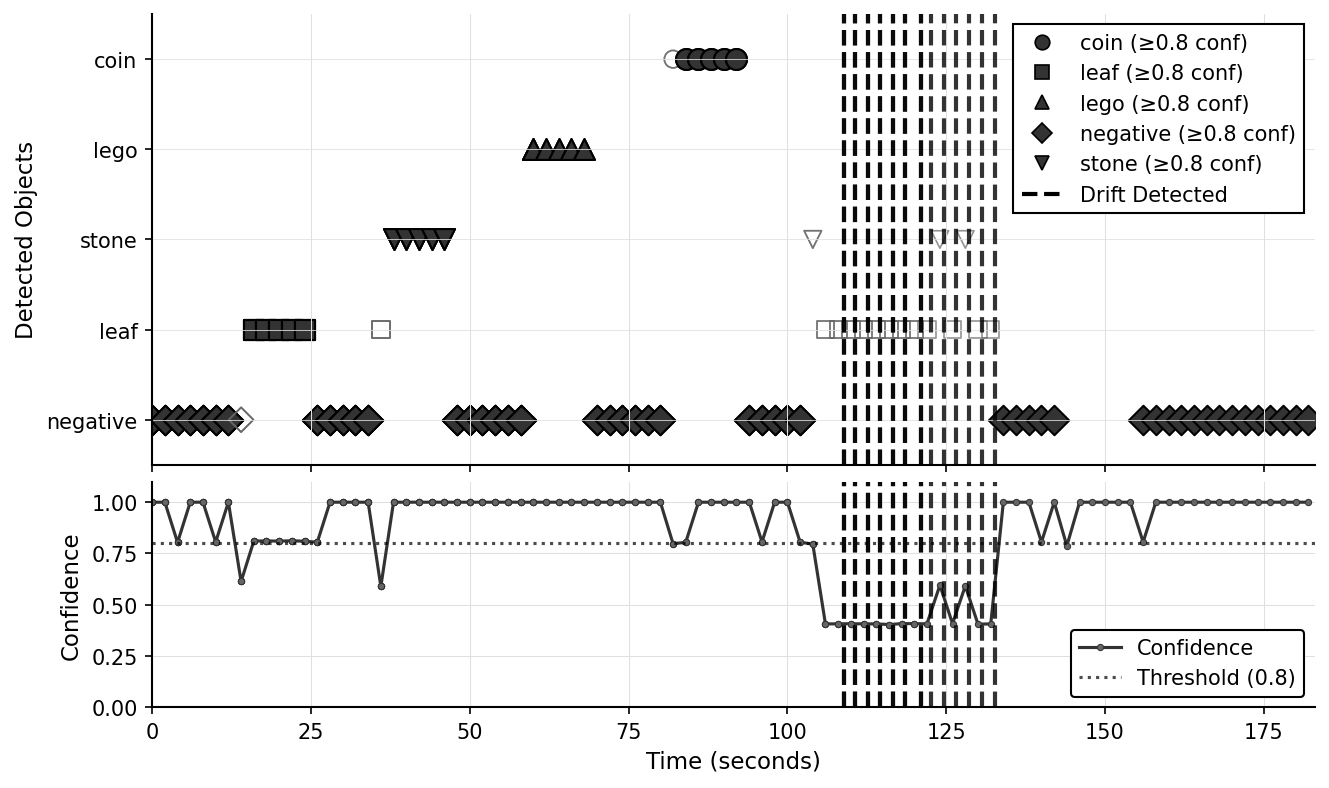
\includegraphics[width=.98\linewidth]{figs/evaluation//drift_ball_timeline.png}
  \caption[Drift Prediction Timeline for Scenario S2 (Single Drift)]{Prediction timeline and drift alarms for Scenario S2 (Single Drift). Visual encoding is the same as in Figure~\ref{fig:timeline-exp1_s1}. In this scenario, ``coin'' is a known class, and only ``ball'' represents a novel drift object.}
  \label{fig:timeline-exp2_s2}
\end{figure}

\begin{figure}[htbp]
  \centering
  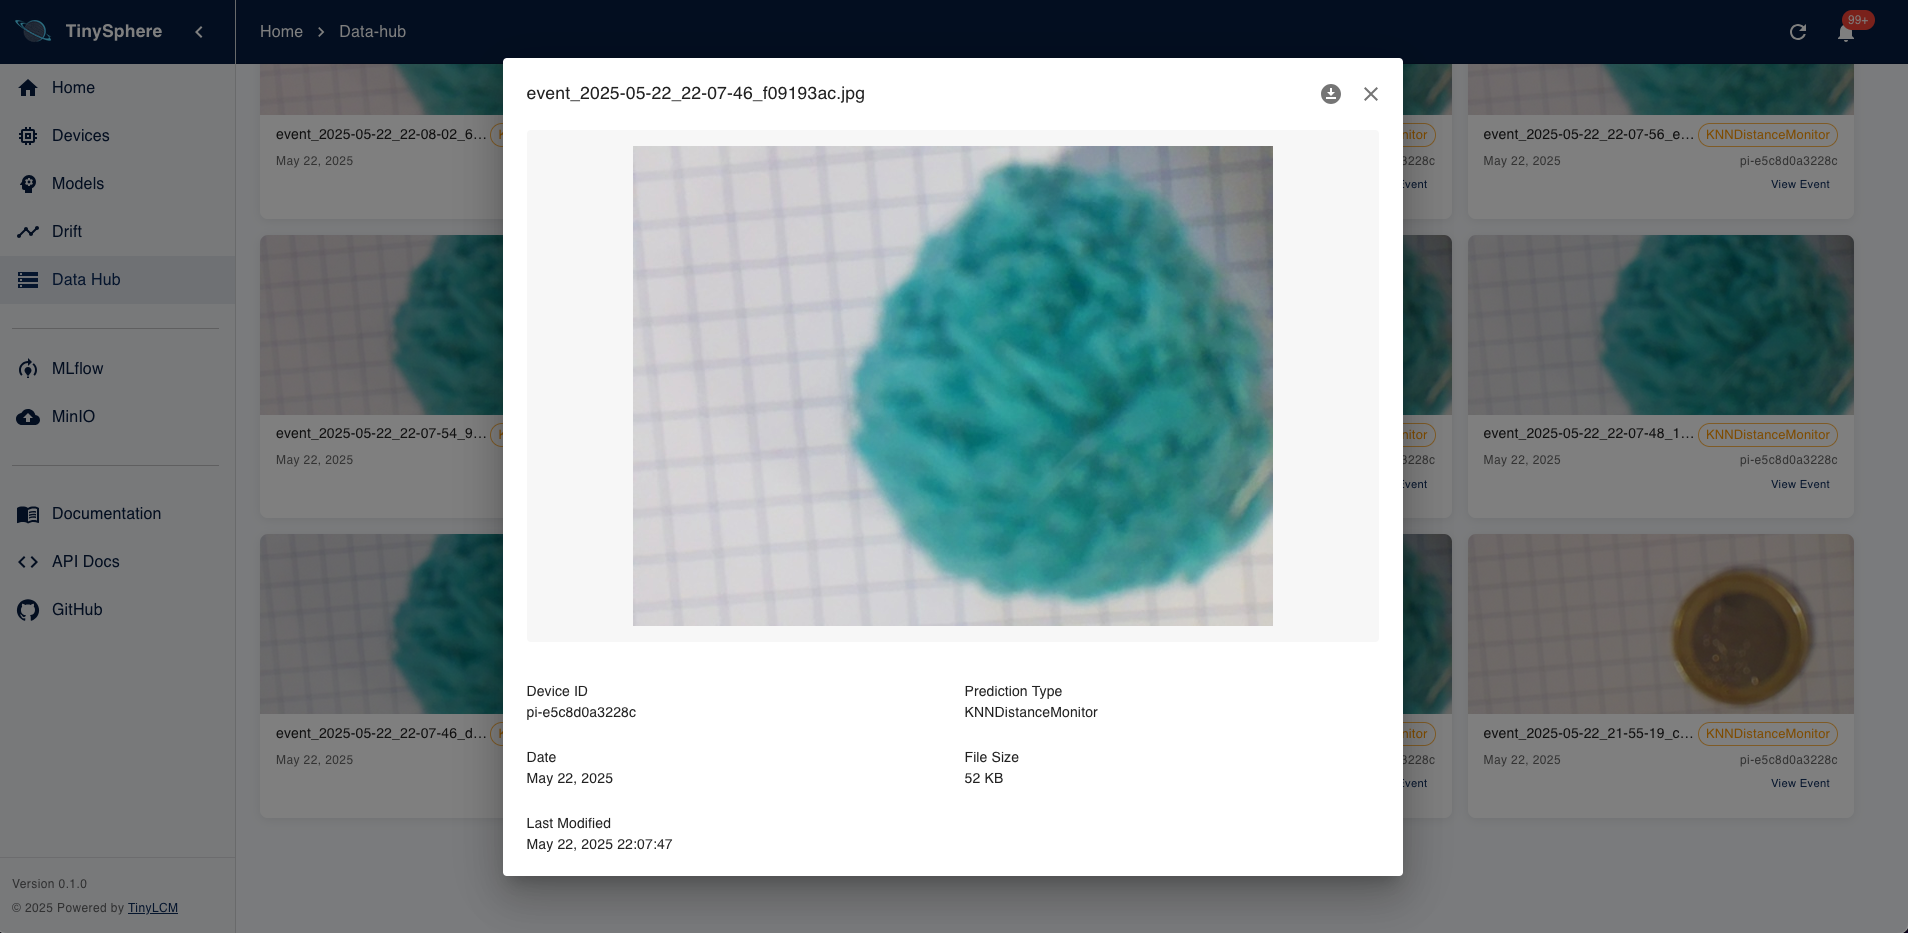
\includegraphics[width=0.59\linewidth]{figs/evaluation/drift_image_exp2_ball.png}
  \caption[Drift Image of Scenario 2 (Single Drift)]{Example of a drift-flagged image (object: ``ball'') from Scenario S2, where ``coin'' was a known class.}
  \label{fig:drift-image-ball-s2}
\end{figure}

\subsection{Quantitative Analysis and Hypothesis Testing (H$_3$)}
\label{ssec:phase2_quantitative_drift_metrics}

To provide a robust assessment beyond qualitative inspection, a quantitative analysis was performed. Each drift check operation was classified into a 2x2 confusion matrix. The results, along with the p-values from the Fisher's Exact Test used to evaluate H$_3$, are consolidated in Table~\ref{tab:drift_detection_combined_results}.

\begin{table}[htbp]
    \centering
    \caption[Quantitative Drift Detection Results and Hypothesis Test for H$_3$]{Summary of drift detection performance and results of the Fisher's Exact Test for H$_3$.}
    \label{tab:drift_detection_combined_results}
    \footnotesize
    \setlength{\tabcolsep}{4pt}
    \begin{tabularx}{\linewidth}{@{} X c c c c r @{}}
        \toprule
        \textbf{Scenario} & \textbf{TP} & \textbf{FN} & \textbf{FP} & \textbf{TN} & \textbf{$p$-value} \\
        \midrule
        S1: Dual Drift (coin \& ball) & 8 & 20 & 10 & 146 & $0.0016$ \\
        S2: Single Drift (ball) & 20 & 6 & 0 & 158 & $8.26\times10^{-22}$ \\
        \bottomrule
    \end{tabularx}
\end{table}

The Fisher's Exact Test for both scenarios yielded statistically significant p-values ($p < 0.05$), as shown in Table~\ref{tab:drift_detection_combined_results}. This confirms a strong, non-random association between the presentation of an untrained object and the triggering of a drift alarm in both cases. Based on this evidence, \textbf{H$_3$ is accepted}.

The acceptance of H$_3$ formally validates the core capability of the \gls{tinylcm} framework: it can detect statistical drift in a manner that is statistically significant. The system can reliably distinguish drift periods from non-drift periods.

However, a separate analysis of the system's sensitivity reveals further insights. The True Positive Rate (TPR) for S1 was 28.6\% (8 out of 28 drift events detected), and for S2, it was 76.9\% (20 out of 26 events detected). This discrepancy highlights a key finding: the system's performance is highly dependent on the nature of the drift and the behavior of the base model.

In Scenario S1, which included the ``coin'' as a second drift object, the sensitivity dropped, and the number of false positives increased. This suggests that the feature representation of the ``coin'' may be less distinct. Consequently, the k-NN distances were likely only marginally or inconsistently higher than the baseline, preventing the Page-Hinkley test from accumulating enough evidence to reliably trigger an alarm. A closer examination of the timeline in Figure~\ref{fig:timeline-exp2_s1} reveals that at the beginning of the ``ball's''s presentation, the base model repeatedly misclassified the novel object as ``lego'' with a high confidence score (approx. 0.8). According to the framework's configuration, the drift check is intentionally bypassed for any prediction exceeding this confidence threshold to save computational resources. Therefore, the poor initial performance of the base model directly masked the drift from the downstream \texttt{KNNDistanceMonitor}. The drift detection only commenced later when the base model's confidence for the misclassification dropped.


\section{Cross-Phase Discussion of Results}
\label{sec:cross_phase_discussion_results}

The empirical evaluation provides key insights into the capabilities and trade-offs of the \gls{tinylcm} framework on a resource-constrained device.

Phase 1 confirmed that \gls{tinylcm}, even with active drift detection, operates within the predefined resource budgets (H$_1$ and H$_2$ accepted). The latency overhead, while statistically significant, remained well below the 50\% threshold. The latency breakdown identified feature processing and \gls{knn} classification as the primary contributors, while the drift check mechanism itself added minimal direct overhead.

Phase 2 provided a quantitative validation of the core drift detection function. By demonstrating a statistically significant correlation between the presentation of untrained objects and the generation of alarms (H$_3$ accepted), the evaluation confirms that the \gls{knn}-based monitoring approach is fundamentally sound. The system is not merely guessing; it is responding to genuine statistical deviations in the feature space.

Synthesizing these findings reveals a central trade-off. \gls{tinylcm} successfully provides a statistically valid drift signal without violating strict performance constraints. However, the Phase 2 discussion highlights that the practical effectiveness of this detection is not constant. It varied significantly depending on the characteristics of the novel object. This implies that while the performance cost of the drift check is low and acceptable (Phase 1), the quality of the resulting detection (Phase 2) is highly dependent on system parameters (like the KNN distance threshold) and the nature of the drift itself. The framework thus offers a tunable, low-overhead mechanism, but achieving high sensitivity for diverse drift types requires careful parameterization and potentially more sophisticated distance metrics, representing a classic trade-off between resource cost, detection robustness, and sensitivity.

\section{Result-Level Threats to Validity}
\label{sec:result_level_threats_validity}

Beyond the general threats to validity inherent in the experimental design (discussed in Chapter~\ref{chp:Research_Design}, Section~\ref{ssec:evaluation_threats_to_validity}), the specific results obtained and their interpretation are subject to further considerations that may impact their generalizability or precision:

\begin{itemize}[noitemsep, topsep=0pt]
    \item \textit{Sensitivity to Drift Detection Parameters and Object Characteristics:} The quantitative results from Phase 2 demonstrated that the detector's sensitivity (TPR) varied significantly between scenarios (28.6\% vs. 76.9\%). This confirms that the framework's performance is highly sensitive to both its internal parameters (e.g., the Page-Hinkley test threshold) and the specific features of the drift object. The parameters were not exhaustively optimized, and the performance on more subtle drift types remains an open question.

    \item \textit{Specificity of ``Drift'' Objects:} The novel objects used (``coin'', ``ball'') were chosen to be visually distinct. While effective for validating the fundamental detection capability, this selection does not cover the full spectrum of concept drift. The framework's performance on more gradual changes or on new objects visually similar to known classes was not explicitly tested.

    \item \textit{Experimental Run Order and Potential Carry-over Effects:} As noted in the methodological reflection in Section~\ref{sec:phase1_results_overhead}, the non-randomized execution order of Phase 1 configurations presents a potential threat to internal validity regarding the precise resource differences observed between the two \gls{tinylcm} configurations.
\end{itemize}
Despite these limitations, the controlled experiments provide strong, quantitative evidence for the feasibility of \gls{tinylcm}'s core functionalities on resource-constrained hardware.


%!TEX root = thesis.tex

\chapter{Discussion}
\label{chp:Discussion}

This chapter synthesises the entire study and evaluates how the proposed TinyMLOps ecosystem answers the research questions. It links the empirical results to the wider literature, discusses limitations, and outlines avenues for future work.

~\\
\vfill
\minitoc
\clearpage


\section{Evaluating the TinyMLOps Ecosystem}
\label{sec:evaluating_ecosystem}

This section evaluates the effectiveness of the proposed \gls{tinymlops} ecosystem, encompassing \gls{tinylcm} and TinySphere, in enabling autonomous \gls{lcm}. This evaluation directly addresses the RQ3. The discussion will focus on the ecosystem's design philosophy, its architectural contributions to autonomous operations, its effectiveness across key \gls{lcm} phases, and a comparative analysis against existing solutions.

\subsection{Philosophy and Architectural Design}
\label{ssec:autonomy_first_philosophy}

A central design principle is the ``autonomy-first'' philosophy: the on-device component, \gls{tinylcm}, holds the primary intelligence for managing the model lifecycle.  
This mitigates the cloud-dependency seen in many \gls{tinyml} deployments and is essential for intermittently connected scenarios such as the Mars-rover case study.  \gls{tinylcm} therefore follows a data-centric pipeline with modular blocks for feature extraction, unsupervised drift detection (\texttt{KNNDistanceMonitor}), lightweight classification (\texttt{LightweightKNN}), and robust state management (\texttt{AdaptiveStateManager}).  The successful validation of autonomous drift detection confirms this approach.
  
While \gls{tinylcm} champions on-device self-sufficiency, the ecosystem design pragmatically acknowledges that certain advanced \gls{mlops} capabilities are impractical or overly resource-intensive for isolated, constrained devices. The TinySphere platform serves as an optional, server-side complement, designed to provide these enhanced functionalities without undermining \gls{tinylcm}'s core operational autonomy. This addresses the need for more powerful \gls{mlops} tools, a requirement often met by cloud services in existing literature \cite{banburyEdgeImpulseMLOps2023,alselekAgileAIFirmware2024}. The interaction between \gls{tinylcm} and TinySphere is governed by an opportunistic client-server model, where \gls{tinylcm} functions independently and attempts server communication only when connectivity is available and such interaction is deemed beneficial.

This dual-component architecture, balancing maximal on-device autonomy with optional centralized support, represents a pragmatic approach rather than a compromise. Purely autonomy for all conceivable \gls{mlops} tasks remains a formidable challenge, particularly under severe resource constraints. The literature review in Chapter~\ref{chp:Research_Results} indicated that many existing edge systems still maintain dependencies on cloud components for significant operational aspects. The proposed ecosystem's architecture, by offering a spectrum of operational modes, provides a flexible solution. It allows deployments to function effectively in completely disconnected environments, while also enabling them to leverage richer, server-assisted \gls{mlops} capabilities when connectivity permits. This adaptability makes the ecosystem potentially suitable for a broader range of use cases compared to solutions that are either exclusively device-centric or heavily reliant on continuous cloud integration.

\subsection{Effectiveness in Key Lifecycle Management Phases}
\label{ssec:effectiveness_lcm_phases}

The proposed \gls{tinymlops} ecosystem aims to support multiple phases of the \gls{ml} model lifecycle autonomously on the edge device.

\textbf{Deployment}\quad
While the primary focus of \gls{tinylcm} is on post-deployment \gls{lcm}, its initial setup and configuration, as detailed in Phase 2 of the exemplary operational workflow (Section~\ref{ssec:ecosystem_workflow} in Chapter~\ref{chp:Framework}), facilitate the deployment of an autonomous operational agent on the target device. The provision of configuration files and initial state artifacts allows for a structured instantiation of the \gls{tinylcm} pipeline. 

\textbf{Monitoring} \quad
A cornerstone of \gls{tinylcm}'s autonomous capabilities is its unsupervised drift detection mechanism. The \texttt{KNNDistanceMonitor}, employing the Page-Hinkley statistical test on  \gls{knn} distances within a PCA-transformed feature space, enables continuous monitoring for concept drift without requiring ground truth labels. The empirical evaluation in Chapter~\ref{chp:Evaluation} successfully validated this capability, demonstrating its functional efficacy in controlled laboratory settings. This is particularly significant for \gls{tinyml} scenarios where real-time, labeled data streams are often unavailable, a challenge highlighted in the framework design. 

\textbf{Adaptation} \quad
On-device adaptation is conceptually in place—an \texttt{HeuristicAdapter} quarantines anomalous samples, pseudo-labels them, and (optional after expert validation via TinySphere) updates the \texttt{LightweightKNN}.  

\textbf{Rollback} \quad
To ensure operational resilience, particularly in the context of potentially imperfect autonomous adaptations, \gls{tinylcm} incorporates the \texttt{AdaptiveStateManager}. This component is designed to version critical states, primarily the \texttt{LightweightKNN} classifier's reference set, and persist these snapshots to non-volatile storage. The use of an asynchronous worker thread for save operations, as illustrated in Chapter~\ref{chp:Framework} (Listing~\ref{lst:statemanager}), is a practical consideration, preventing the main inference pipeline from stalling. This rollback capability is vital for maintaining system stability and reliability, allowing the device to revert to a known-good state if an adaptation proves detrimental.

\subsection{Comparison with Existing TinyMLOps Solutions}
\label{ssec:comparison_existing_solutions}

\Gls{tinylcm} is designed to provide an end-to-end perspective for on-device operations, covering monitoring, adaptation, and state management locally. This contrasts with many platforms that, while targeting edge deployment, still rely heavily on cloud infrastructure for core \gls{mlops} tasks like continuous monitoring or model retraining. 
The focus on unsupervised drift detection within \gls{tinylcm} is another key differentiator. \Gls{tinylcm}'s \texttt{KNNDistanceMonitor} provides a mechanism for detecting changes in data distribution without such labels, a crucial capability for truly autonomous systems in label-scarce environments.

Furthermore, the integrated nature of the \gls{tinylcm} and TinySphere ecosystem offers a unique value proposition. TinySphere is not a generic \gls{mlops} backend merely retrofitted for \gls{tinyml}; it is conceptualized as a server-side platform specifically designed to understand, interact with, and augment the autonomous operations of \gls{tinylcm}-enabled devices. This synergy—supporting opportunistic communication, facilitating validation of on-device decisions, and providing \gls{tinyml}-aware fleet management—differs from approaches that might use general-purpose tools like MLflow in isolation or platforms that offer less specialized support for the nuances of autonomous edge device operations.

\section{Critical Examination of Research Findings}
\label{sec:critical_examination_findings}

This section critically examines the research findings presented throughout the thesis, synthesizing how they collectively address the posed research questions. It also discusses the broader significance of these findings and compares them against the claims made by the proposed framework and the existing body of literature.

\subsection{Addressing the Research Questions}
\label{ssec:addressing_rqs}

The research was structured around four key questions, and the findings from various chapters contribute to answering them in an interconnected manner, reflecting the iterative nature of the \gls{dsr} methodology employed.

\paragraph{RQ1: What system architectures, methodologies, and practices are employed to support \gls{tinyml} in resource-constrained embedded systems?}
This question was primarily addressed by the systematic literature analysis presented in Chapter~\ref{chp:Research_Results}. The findings revealed a predominance of Data-Centric and Client-Server architectural patterns. Methodologically, Centralized Training and Offline Learning for statically pre-trained models were common, though an increasing interest in decentralized and on-device learning was noted. Common hardware platforms often included more capable \glspl{mcu} and \glspl{sbc} for tasks like sensor-based analysis, computer vision, and audio processing. Findings are highlighted in Chapter~\ref{chp:Research_Results} (\ref{sec:RQ1_Results_SystemArchitecture}) These insights directly informed the design choices for the proposed ecosystem: \gls{tinylcm} adopts a data-centric pipeline architecture, and its interaction with TinySphere follows a client-server model, initially supporting centrally trained models but designed with future on-device adaptation in mind. The selection of the Raspberry Pi Zero 2W, an \gls{sbc}, for the empirical evaluation also aligns with the observed trend of using more capable, yet still constrained, hardware for complex \gls{tinyml} tasks.

\paragraph{RQ2: Which frameworks and strategies facilitate decentralized on-device \gls{mlops} while minimizing reliance on cloud infrastructure?}
Chapter~\ref{chp:Research_Results} also addressed this question by identifying and categorizing existing frameworks and strategies that support aspects of decentralized on-device \gls{mlops}, such as on-device learning, model adaptation, and \gls{ota} updates. Findings are highlighted in Chapter~\ref{chp:Research_Results} (\ref{sec:RQ2_Results_Frameworks}). The analysis highlighted a growing momentum towards greater on-device intelligence. However, it also revealed a degree of fragmentation, with many solutions focusing on specific aspects of \gls{mlops} rather than providing a comprehensive, integrated on-device \gls{lcm} solution. This identified gap underscored the need for a framework like \gls{tinylcm}, which aims for broader on-device \gls{lcm} coverage, and a \gls{tinyml}-aware server backend like TinySphere to support these autonomous devices in a cohesive manner.

\paragraph{RQ3: How can a \gls{tinymlops} framework be designed to enable effective on-device model \gls{lcm} in resource-constrained systems?}
This question is the central design challenge of the thesis and is primarily answered by the conceptual design of the \gls{tinylcm} and TinySphere ecosystem presented in Chapter~\ref{chp:Framework}. The proposed solution involves \gls{tinylcm}'s modular architecture with components for feature processing, lightweight classification, unsupervised drift detection, state management for rollbacks, and a conceptual mechanism for heuristic-based on-device adaptation. TinySphere complements this with server-side capabilities for data aggregation, validation, and fleet management. The effectiveness of this design in enabling on-device \gls{lcm} is partially demonstrated by the successful empirical validation of \gls{tinylcm}'s drift detection and its performance within resource constraints (Chapter~\ref{chp:Evaluation} ).

\paragraph{RQ4: How does deploying on-device TinyMLOps in decentralized embedded systems influence deployment complexity, resource consumption, and performance trade-offs?}
The empirical evaluation detailed in Chapter~\ref{chp:Evaluation} provides direct answers to this question regarding the \gls{tinylcm} framework.
Deployment Complexity: The exemplary workflow (Phase 2 in Section~\ref{ssec:ecosystem_workflow}) outlines a deployment process involving device preparation, automated installation via scripts, and configuration file management. While this process can be streamlined, it still entails multiple steps, indicating a moderate level of initial deployment complexity.
The evaluation confirmed that \gls{tinylcm} operates within acceptable resource limits on a Raspberry Pi Zero 2W. The inference latency overhead introduced by \gls{tinylcm} components was below the 50\% threshold relative to baseline \gls{tfl} inference (Hypothesis H$_1$ accepted). The latency breakdown revealed that feature extraction and \gls{knn} classification are the primary contributors to this overhead. The observed mean inference latency of approximately 420-436 ms (around 2.3 frames per second) is suitable for some near real-time applications but may be a limiting factor for others requiring faster responses. This highlights a fundamental trade-off: the valuable capability of on-device intelligence (specifically, unsupervised drift detection) comes at a quantifiable computational cost, which \gls{tinylcm} is designed to manage within the constraints of platforms like \glspl{sbc}.

The systematic progression from understanding the problem domain (RQ1, RQ2 via literature analysis), to designing an artifact (RQ3 via framework development), and finally to evaluating that artifact (RQ4 via empirical testing) clearly reflects the \gls{dsr} methodology outlined in Chapter~\ref{chp:Research_Design}. This structured approach ensures that the proposed framework is not only theoretically grounded but also practically assessed, with findings from each stage informing the next.

\subsection{Significance of the Findings}
\label{ssec:significance_findings}

The research findings carry several significant implications for the field of \gls{tinymlops}.
Firstly, the work contributes to advancing the feasibility of more autonomous \gls{tinyml} systems. The design of \gls{tinylcm}, demonstrates a practical pathway towards reducing the reliance of edge devices on continuous network connectivity and cloud-based intervention for core monitoring tasks. This is especially relevant for applications in remote or challenging environments, such as the motivating Mars rover scenario, where autonomy is paramount. By enabling devices to locally sense and react to changes in their operational context, this research helps extend the reach of data-driven methods to settings previously constrained by connectivity limitations.

Secondly, the \gls{tinylcm} framework offers a practical approach for on-device monitoring in label-scarce environments. The successful validation of its unsupervised drift detection mechanism provides a tangible tool for an important \gls{mlops} phase.

Thirdly, the conceptualization of TinySphere provides a blueprint for TinyML-centric server-side support. Instead of merely adapting generic cloud \gls{mlops} tools, TinySphere is envisioned as a platform specifically designed to interact with, manage, and augment fleets of autonomous \gls{tinyml} devices. This addresses a noted gap for server infrastructure that understands the unique data streams and operational modes of such edge systems.

Finally, the empirical performance benchmarks obtained from evaluating \gls{tinylcm} on a Raspberry Pi Zero 2W offer concrete data points for the research community and practitioners. These benchmarks provide valuable insights into the tangible costs and capabilities associated with implementing on-device \gls{mlops} features on representative \gls{sbc} hardware.

Beyond these direct technical contributions, the overarching significance lies in potentially enabling new classes of \gls{tinyml} applications or enhancing existing ones. As stated in the introduction, \gls{tinyml} aims to bring intelligence to the very edge, to devices limited by power, connectivity, or form factor. A framework that enhances the operational autonomy and resilience of these devices, by allowing them to manage their \gls{ml} models more self-sufficiently, directly supports this goal.

\subsection{Comparison with Broader Literature and Framework Claims}
\label{ssec:comparison_literature_claims}

The research presented in this thesis aligns with the broader trend identified in the literature (Chapter~\ref{chp:Research_Results}) towards greater on-device intelligence and more edge-native \gls{mlops} capabilities. The proposed ecosystem specifically endeavors to address certain gaps.

When evaluating the claims made for the framework in Chapter~\ref{chp:Framework} :

\begin{itemize}
    \item \textit{\gls{tinylcm} enables autonomous \gls{lcm}:} This claim is partially met. The empirical evaluation demonstrated autonomous unsupervised drift detection. The design includes mechanisms for state management and rollback. However, the on-device adaptation component, crucial for fully autonomous \gls{lcm}, remains conceptual and was not empirically validated for its autonomous learning capabilities.
    
    \item \textit{Minimal cloud reliance:} This claim is largely met for \gls{tinylcm}'s core operational loop, particularly for monitoring. Interaction with TinySphere is designed to be opportunistic, allowing \gls{tinylcm} to function independently.
    
    \item \textit{Suitable for resource-constrained devices:} The empirical evaluation was conducted on a Raspberry Pi Zero 2W. While this demonstrates feasibility on such platforms, the direct applicability and performance of the current Python-based \gls{tinylcm} implementation on more severely constrained \gls{mcu}s (typically programmed in C/C++) are not directly proven by this evaluation. While \gls{tfl} can target \gls{mcu}s, porting the entire \gls{tinylcm} Python framework would require significant effort and likely reimplementation. This distinction needs to be carefully considered when assessing suitability across the full spectrum of \gls{tinyml} hardware. 
\end{itemize}

\section{Limitations of the Research}
\label{sec:limitations_research}

While this research contributes to the field of \gls{tinymlops}, it is important to acknowledge its inherent limitations, which span the methodological approach, the design of the proposed framework, and the scope of its empirical evaluation.

The \gls{dsr} methodology, while well-suited for developing and evaluating novel artifacts such as the TinyMLOps ecosystem, has practical constraints within the confines of a thesis. The iterative design, implementation, and evaluation cycles may not achieve the same depth or breadth as a larger, long-term research project. For example, the initial exploration of the problem space could potentially have benefited from a wider range of inputs or alternative framings to further enrich the understanding of requirements. Furthermore, the literature review process, which combined \gls{sms} and \gls{slr} techniques as detailed in Chapter~\ref{chp:Research_Design}, is subject to the common limitations of such reviews. These include the potential for selection bias in the chosen databases or search terms, the risk of overlooking relevant grey literature, and the inherent subjectivity in the interpretation and synthesis of selected studies, despite efforts to maintain rigor through predefined protocols and criteria.

The conceptual design of the TinyMLOps ecosystem, also has limitations. The on-device heuristic adaptation mechanisms within \gls{tinylcm}, designed for autonomous learning and concept drift response, are largely conceptual at this stage. While the architectural groundwork and component interactions were defined, the specific algorithms for pseudo-label generation and their robust, resource-efficient implementation on diverse \glspl{mcu} were not fully realized or empirically tested. This means that the framework's capacity for fully autonomous, unsupervised adaptation in complex, real-world scenarios remains an area for substantial future development and validation. Similarly, TinySphere's capabilities for processing and validating data originating from these advanced on-device adaptations are, by extension, also based on this conceptual foundation. Although TinySphere integrates established MLOps tools like MLflow and provides a structured approach to TinyML-specific data, the complete end-to-end feedback loop involving sophisticated server-side validation of on-device heuristic learning and subsequent automated model refinement on the edge device has not been fully implemented and evaluated.

The empirical evaluation of the \gls{tinylcm} framework, as presented in Chapter~\ref{chp:Evaluation}, was conducted under controlled laboratory conditions using a Raspberry Pi Zero 2W as the target platform. While this setup allowed for reproducible measurements of performance overhead and a qualitative assessment of drift detection efficacy, its external validity is constrained. The results may not directly generalize to the wide variety of even more resource-constrained \glspl{mcu} or to different application domains with diverse data characteristics and operational demands. The specific ``drift'' objects used were visually distinct, and the framework's performance on more subtle or gradual concept drift types was not exhaustively tested. Additionally, while the performance overhead was found to be acceptable against predefined thresholds, the absolute latency on the Raspberry Pi Zero 2W might be too high for applications requiring very fast real-time responses.

%!TEX root = thesis.tex

\chapter{Conclusion}
\label{chp:Conclusion}

This thesis was dedicated to the conception, development, and evaluation of a novel ecosystem for the lifecycle management of machine learning models on severely resource-constrained embedded systems, known as \gls{tinyml}. Stemming from the observation that traditional \gls{mlops} approaches do not adequately address the specific challenges of \gls{tinyml} environments—particularly limited computational power, low memory, scarce energy budgets, and often unreliable network connectivity—a system was designed that aims for maximum on-device autonomy with optional, synergistic server-side support. The original motivation was to reduce dependence on cloud infrastructures, thereby expanding the applicability of \gls{tinyml} in scenarios where continuous cloud connectivity cannot be guaranteed, such as in the motivating context of an autonomous Mars rover mission.

This thesis offers several scientific contributions. The systematic literature analysis provided a detailed overview of the current research landscape in \gls{tinymlops}, highlighting the predominance of centralized training and offline learning, the rise of decentralized and on-device learning strategies, the fragmentation of existing solutions, and the lack of comprehensive, empirically validated end-to-end frameworks for autonomous on-device \gls{lcm}. This review underscored the need for the proposed integrated ecosystem. The core innovative contribution is the conceptual design of the \gls{tinymlops} ecosystem, encompassing \gls{tinylcm} and TinySphere. This design is guided by an ``autonomy-first'' philosophy, featuring a modular, data-centric pipeline architecture for \gls{tinylcm} that includes components for feature extraction, resource-efficient \gls{knn} classification, unsupervised drift detection using the \texttt{KNNDistanceMonitor} and the Page-Hinkley test, robust state management for versioning and rollbacks via the \texttt{AdaptiveStateManager}, and a conceptual mechanism for heuristic-based on-device adaptation involving the \texttt{HeuristicAdapter} and \texttt{QuarantineBuffer}. TinySphere is designed as a specialized, \gls{tinyml}-centric server platform that extends beyond generic \gls{mlops} tools by being tailored to process data from \gls{tinylcm} devices, support validation workflows, and enable comprehensive fleet management, all interacting via an opportunistic client-server model. The empirical validation of \gls{tinylcm} furnished concrete evidence of its feasibility and performance, providing quantitative benchmarks for latency and resource usage on representative \gls{sbc} hardware.

The findings of this research bear significant implications for both scientific inquiry and practical application. The work advances the development of more autonomous \gls{tinyml} systems, reducing their dependence on continuous network connectivity and cloud intervention, which is particularly relevant for applications in remote or challenging environments. The validated unsupervised drift detection mechanism in \gls{tinylcm} offers a tangible tool for a critical \gls{mlops} phase, addressing the common issue of unavailable real-time labels in many \gls{tinyml} deployments. The TinySphere concept provides a blueprint for server-side infrastructure specifically designed to interact with autonomous \gls{tinyml} devices, filling a gap in understanding and supporting their unique data streams and operational modes. The empirically determined performance benchmarks serve as valuable references for assessing the costs and capabilities of on-device \gls{mlops} functions. The tension between maximal on-device autonomy and the benefits of centralized \gls{mlops} is a central theme, and the proposed ecosystem attempts to strike a balance, aiming for an intelligent combination rather than an exclusive choice.
%!TEX root = thesis.tex

\chapter{Future Work}
\label{chp:Future_Work}

A central and urgent area for future work arises directly from the on-device adaptation mechanism of \gls{tinylcm}, which was conceptually designed in Chapter~\ref{chp:Framework} (Section~\ref{ssec:tinylcm_drift_adaptation}) and highlighted as a limitation in Chapter~\ref{chp:Discussion}. The ability of a \gls{tinyml} system to autonomously react to detected concept drifts and adapt its model is crucial for maintaining long-term performance and reliability. Future efforts in this domain should concentrate on several key aspects. Firstly, the development and implementation of efficient algorithms for pseudo-label generation is paramount. The heuristic rules and clustering approaches envisioned for the \texttt{HeuristicAdapter} to generate pseudo-labels for anomalous samples collected in the \texttt{QuarantineBuffer} must be meticulously elaborated and implemented in a resource-efficient manner. This necessitates research into lightweight clustering methods suitable for execution on \glspl{mcu} or \glspl{sbc} with limited memory and computational power. Secondly, a robust update of the on-device classifier is required. The mechanisms within the \texttt{AdaptiveHandler} for cautiously updating the \texttt{LightweightKNN} classifier with pseudo-labeled data must be refined, with strategies to prevent catastrophic forgetting and to control the integration of new information being particularly important. Lastly, rigorous empirical validation of the implemented adaptation mechanisms must be undertaken. This includes testing the effectiveness of adaptation to various types of concept drift (abrupt, gradual, recurrent), investigating the long-term stability of the learning process, and analyzing the impact on overall system performance.

In parallel with advancing \gls{tinylcm}'s on-device capabilities, the further development and evaluation of the TinySphere platform and its associated feedback loop are of considerable importance. Future work concerning TinySphere should encompass several directions. A primary focus will be the refinement of interfaces and data exchange mechanisms; the communication protocols and data formats for exchange between \gls{tinylcm} and TinySphere must be optimized to ensure efficiency, robustness, and security, particularly considering intermittent connectivity. Furthermore, the implementation of advanced analysis methods within TinySphere is necessary; it should be equipped with analytical tools to evaluate aggregated data from device fleets, potentially including the automatic detection of global drift patterns, comparative analysis of model performance across different devices and environments, or the identification of systematic error sources. Another key area is the robust implementation of the human-in-the-loop validation workflow. The process for validating on-device generated pseudo-labels by human experts, as outlined in Chapter~\ref{chp:Framework} (Section~\ref{ssec:tinysphere_capabilities}), must be fully implemented. Additionally, the drift classification could also be achived fully automated, by integration better models on server-side, combined with automated orchestration tools such as Airflow.

The empirical evaluation conducted in Chapter~\ref{chp:Evaluation} provided important initial results but is limited in scope. Thus, a significant expansion of this empirical evaluation is required to more comprehensively investigate the robustness and generalizability of the developed solutions. One critical aspect of this expansion is the investigation on more resource-constrained \glspl{mcu}. The evaluation of \gls{tinylcm} to date has been performed on a Raspberry Pi Zero 2W, a relatively capable \gls{sbc}. To demonstrate the framework's applicability to the lower spectrum of \gls{tinyml} hardware, porting and evaluating \gls{tinylcm}, or at least its core components, on typical \glspl{mcu} is essential. This will likely require reimplementation in C/C++, introducing new challenges regarding memory management, computation time optimization, and integration with bare-metal or \gls{rtos} environments. Such investigations would yield valuable insights into the scalability and actual minimum resource requirements of the approach. Furthermore, the applicability to more complex datasets and tasks, such as other sensor data (e.g., time series from accelerometers, audio data) and more demanding \gls{ml} assignments, should be explored. This requires the development of new, more challenging test scenarios and potentially the use of established benchmarking datasets for concept drift detection.

Beyond the core functionalities already addressed, an investigation of additional \gls{mlops} aspects would enhance the practical viability of the \gls{tinymlops} ecosystem. Security and data privacy in on-device operations and data synchronization are critical cross-cutting themes for trustworthy \gls{ai} systems. Future research in this area should address several facets. These include the development of robust mechanisms for secure model and software updates via \gls{ota}, covering \gls{ml} models, adaptation logic, and the \gls{tinylcm} firmware itself. Additionally, an investigation of the vulnerability of on-device models to malicious adversarial attacks and the development of lightweight defense strategies are needed. Finally, ensuring privacy-compliant data aggregation and analysis is essential; this means that the synchronization of data with TinySphere and its analysis must comply with data privacy requirements, for example, through anonymization or pseudonymization techniques, or the use of privacy-preserving machine learning methods. This beed done, \gls{fl} could be explored by enabling collaborative learning across devices without the need for constant data transmission to a central server. This would not only enhance energy efficiency but also improve data privacy by keeping sensitive data on the device. Another vital consideration is the energy efficiency of on-device learning and adaptation processes. Many \gls{tinyml} devices are battery-operated, making energy efficiency a dominant design factor. Future work must meticulously analyze and optimize the energy consumption of on-device learning and adaptation processes, as well as continuous drift monitoring. This could involve the development of energy-aware algorithms, adaptive sampling rates for monitoring, or the utilization of hardware accelerators.

Finally, although the Mars rover mission served as a motivating scenario, future work should investigate the potential application fields and transferability of the results of the developed \gls{tinymlops} ecosystem to other domains. Potential application fields include, but are not limited to, industrial condition monitoring and predictive maintenance, smart agriculture for optimized resource management, personalized medical technology and health monitoring, and autonomous systems in logistics or environmental monitoring. Investigating the specific requirements of these application fields and adapting the ecosystem would demonstrate its broader relevance and the impact potential of the research.

In summary, the present work has laid a solid foundation. The outlined future work aims to bridge the conceptual-empirical gap, enhance the generalizability and robustness of the solution, and integrate important cross-cutting themes such as security and energy efficiency to further increase the practical viability of the \gls{tinymlops} ecosystem.


%%%%%%%%%%%%%%%%%%%%%%%%%%%%%%%%%%%%%%%%%%%%%
%% Text: Appendix
%% If your thesis contains an appendix, uncomment the lines below. The
%% appendix file will be treated like ''ordinary'' chapters...

\printglossary[type=\acronymtype,title=Acronyms]

\appendix
%!TEX root = thesis.tex

\chapter{Appendix}

\section{Detailed AI Use Cases in TinyML Research}
\label{app:detailed-ai-use-cases}

\begin{figure}[htbp]
    \centering
    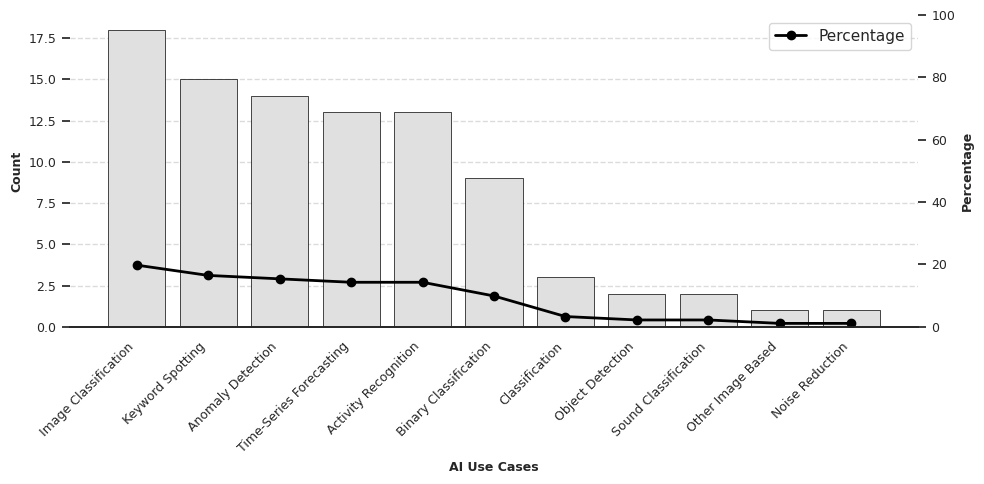
\includegraphics[width=0.98\textwidth]{figs/research_results/ai_use_case_detailed.png}
    \caption[Detailed AI Use Case Distribution]{Fine-grained distribution of AI use cases across the reviewed studies, showing the prevalence of specific applications such as image classification, keyword spotting, and anomaly detection.}
    \label{fig:detailed-ai-use-cases}
\end{figure}

\section{CI/CD Tactics and Optimization Techniques in TinyMLOps}
\label{app:cicd-optim-techniques}

\begin{table}[htbp]
    \centering
    \caption{CI/CD Tactics and Optimization Techniques in TinyMLOps}
    \label{tab:cicd-optim-techniques}
    \begin{tabularx}{\textwidth}{l l X}
        \toprule
        \textbf{Tactic / Technique} & \textbf{Category} & \textbf{Description} \\
        \midrule
        Full Model Update & CI/CD Tactic & Replaces the entire model on the device with a new version. Suitable for significant model changes or retraining. \\
        \midrule
        Partial Model Update & CI/CD Tactic & Updates only specific parts or layers of the model, reducing update size and deployment time. Useful for incremental improvements or fine-tuning. \\
        \midrule
        Automated Deployment & CI/CD Tactic & Automates the process of deploying new models to devices, ensuring efficient and consistent updates across fleets of devices. \\
        \midrule
        Automated Tests & CI/CD Tactic & Integrates automated testing into the CI/CD pipeline to validate model performance and system stability after updates. \\
        \midrule
        Quantization & Optimization Technique & Reduces model precision (e.g., from float32 to int8), decreasing model size and inference latency with minimal accuracy loss. \\
        \midrule
        Pruning & Optimization Technique & Removes less important weights or connections from the model, reducing model size and computational cost. \\
        \midrule
        Knowledge Distillation & Optimization Technique & Trains a smaller "student" model to mimic the behavior of a larger, more complex "teacher" model, transferring knowledge and improving efficiency. \\
        \midrule
        Feature Caching & Optimization Technique & Caches frequently used intermediate feature maps during inference to reduce redundant computations and improve latency. \\
        \midrule
        Adaptive Computation & Optimization Technique & Dynamically adjusts the computational workload based on input complexity or resource availability, optimizing energy consumption and latency. \\
        \midrule
        Test-Time Adaptation & Optimization Technique & Fine-tunes or adapts the model parameters during inference based on individual input samples or local data distributions, improving personalization and robustness to drift. \\
        \bottomrule
    \end{tabularx}
\end{table}
\clearpage

\section{H1 and H2 Evalauation Time Series Data}
\label{app:eval-data}

\begin{figure}[htbp]
    \centering
    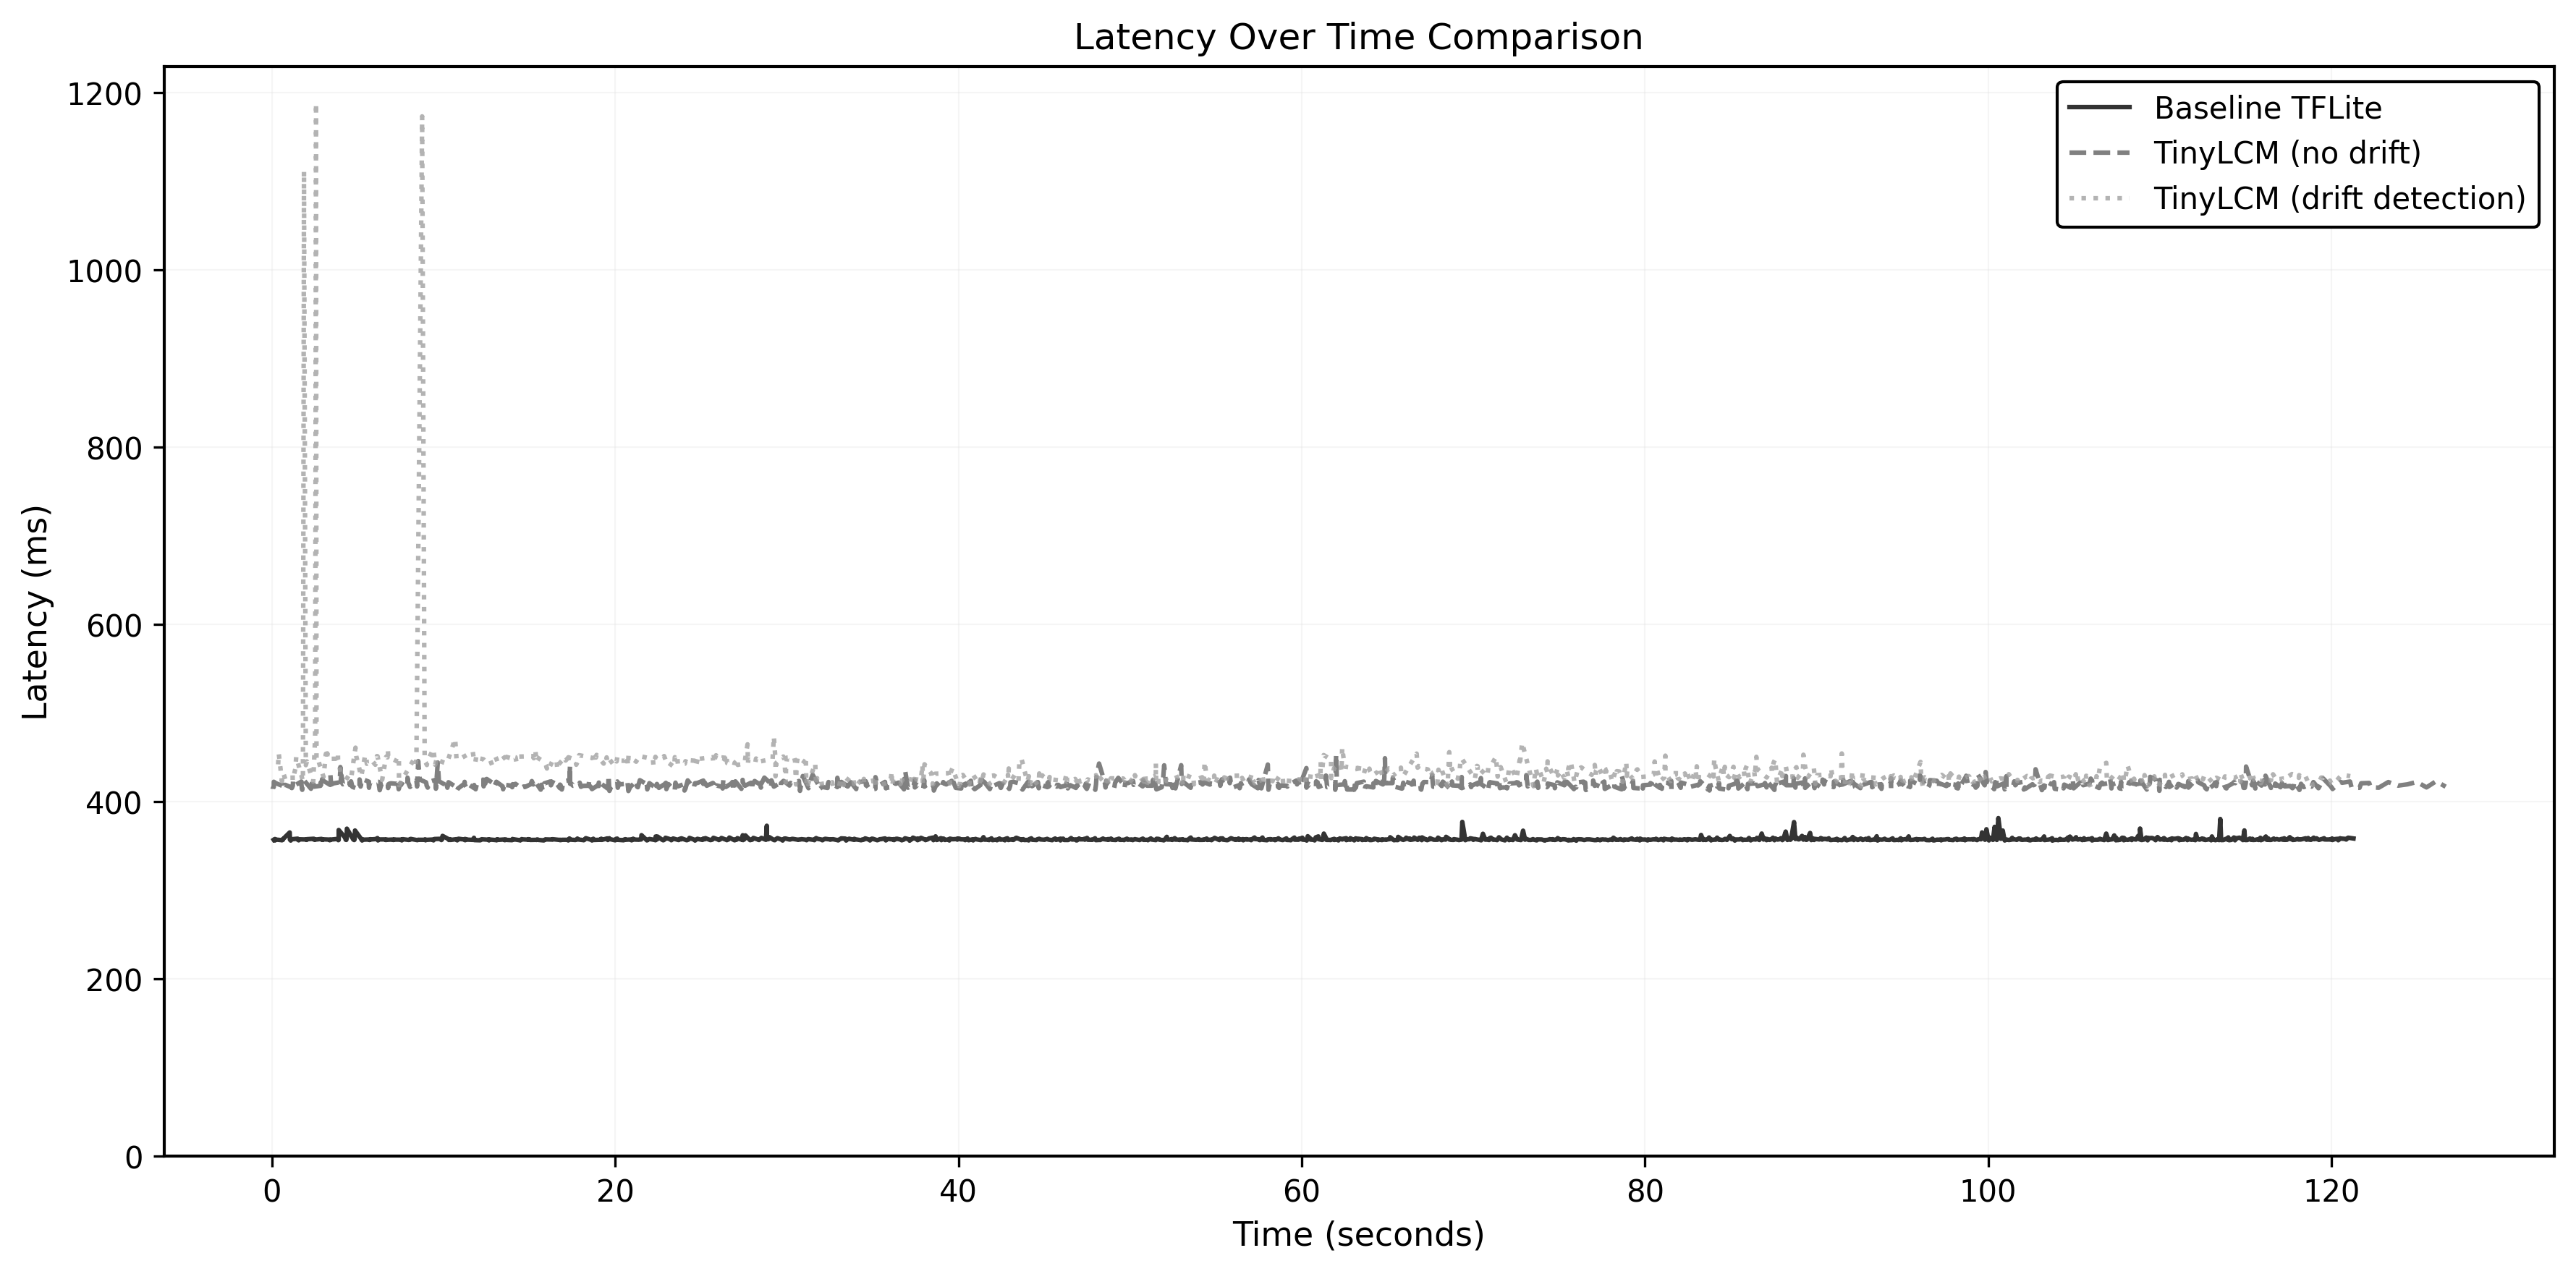
\includegraphics[width=0.98\textwidth]{figs/evaluation/latency_timeseries.png}
    \caption[Latency Comparison]{Time series diagram comparing the latency of the different approaches}
    \label{fig:latency-comparison}
\end{figure}

\begin{figure}[htbp]
    \centering
    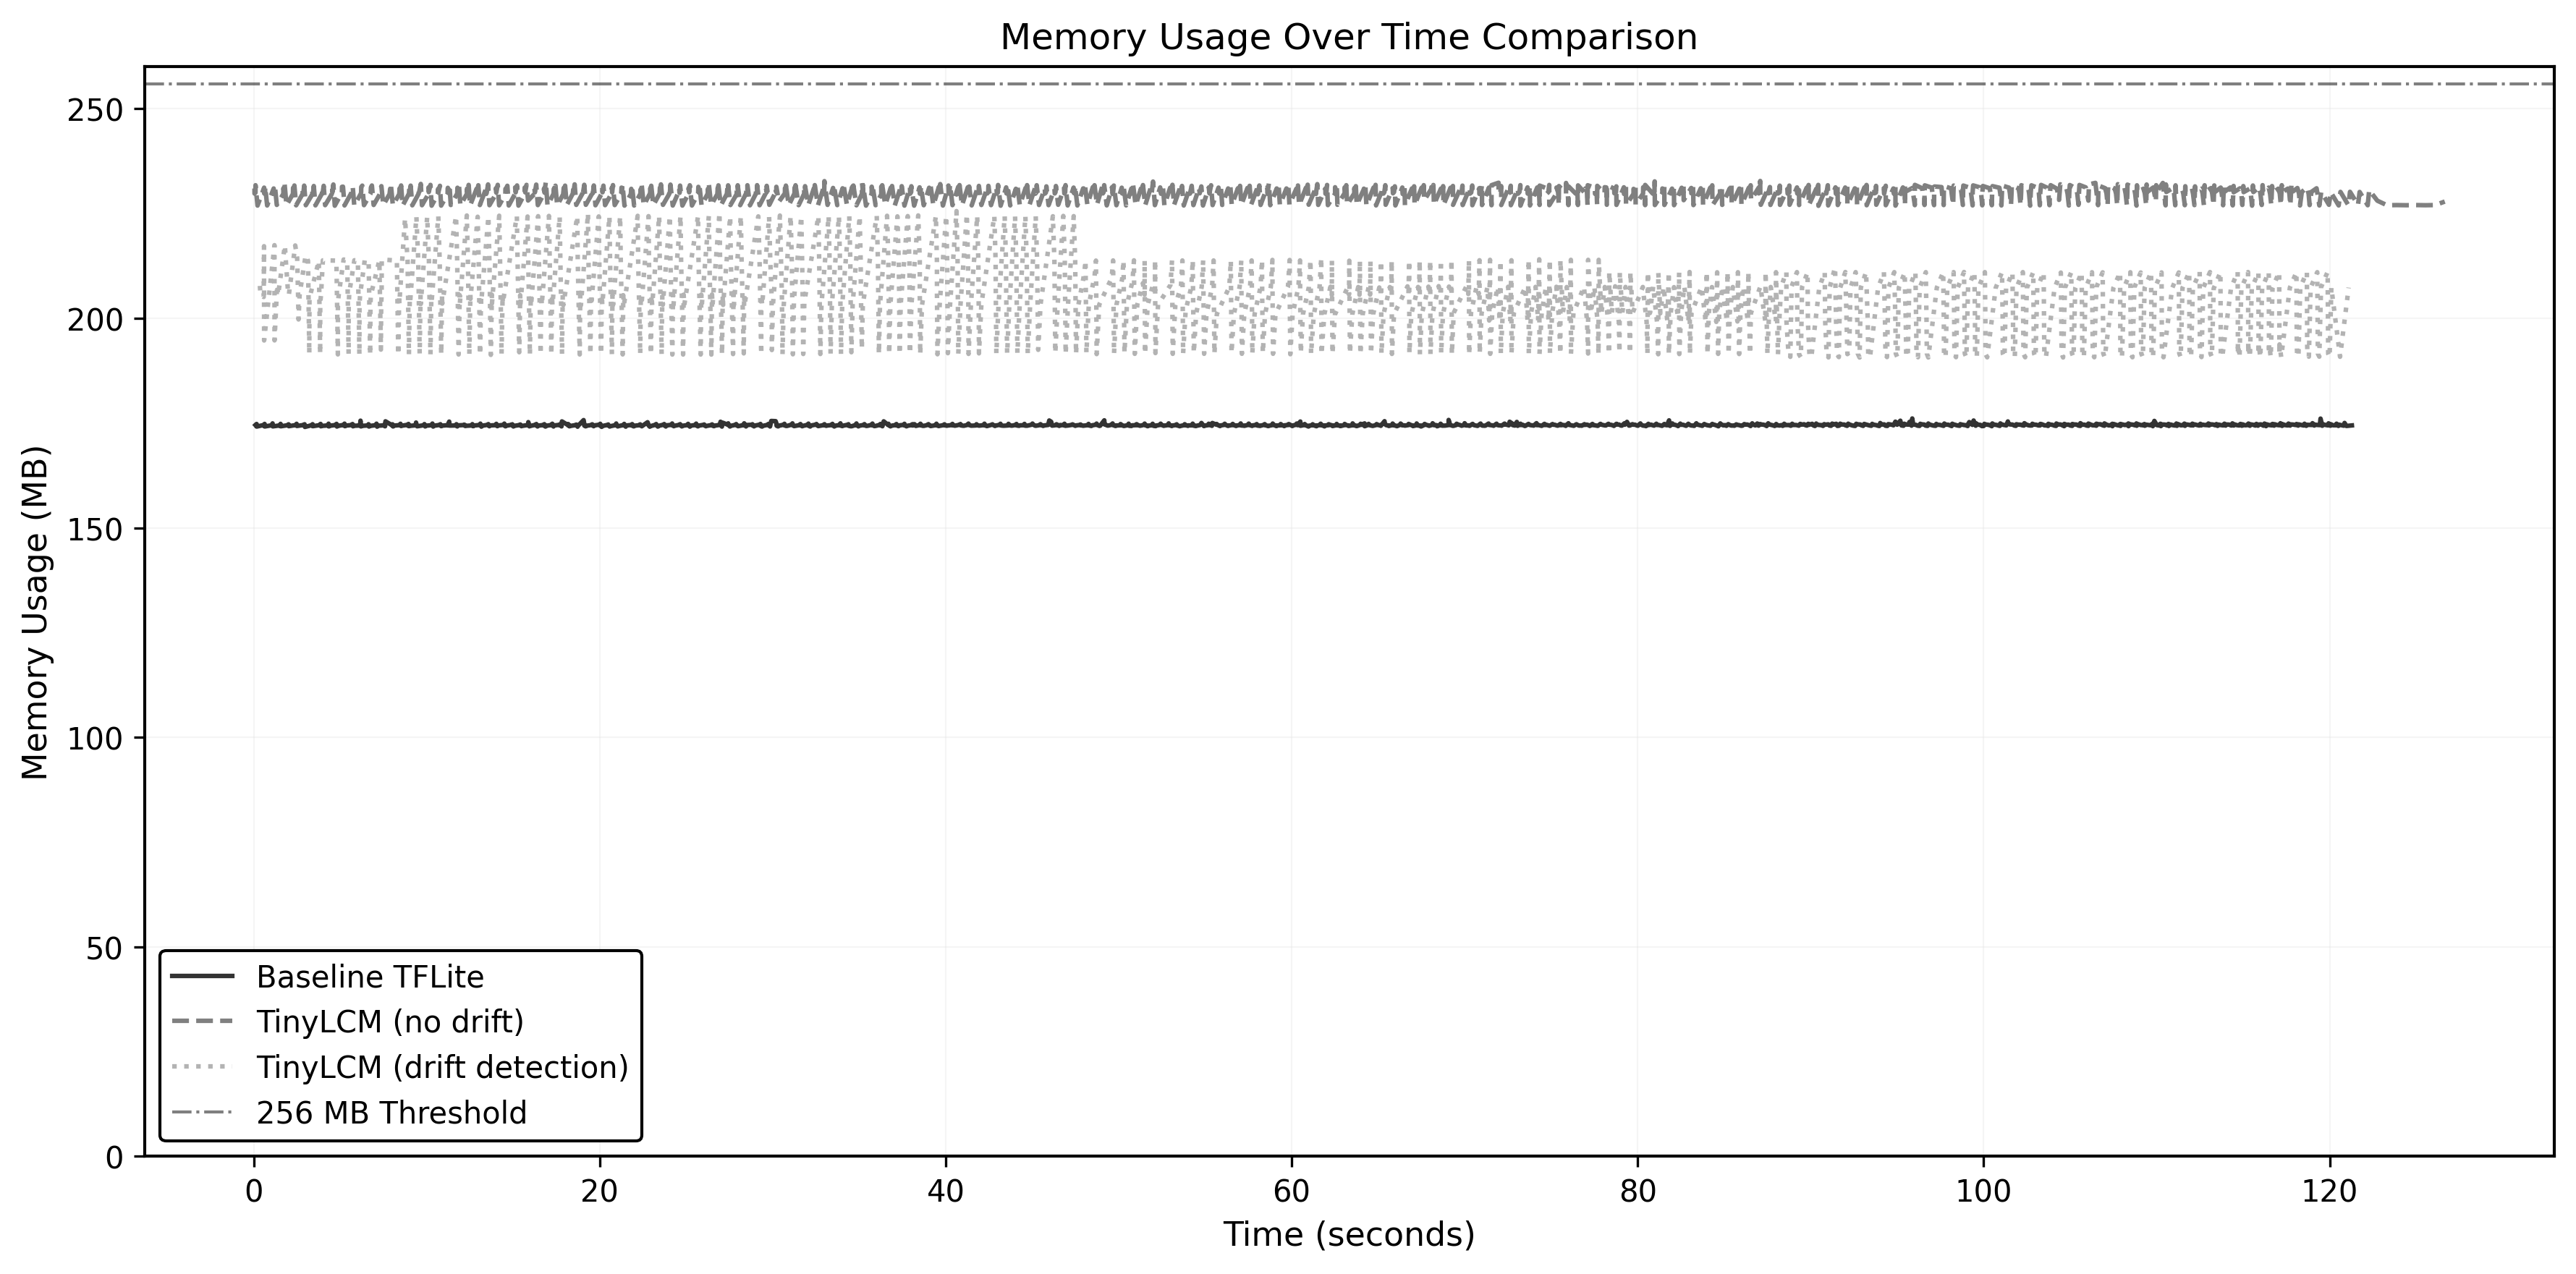
\includegraphics[width=0.98\textwidth]{figs/evaluation/memory_timeseries.png}
    \caption[Memory Comparison]{Time series diagram comparing memory usage of the different approaches}
    \label{fig:memory-comparison}
\end{figure}

\begin{figure}[htbp]
    \centering
    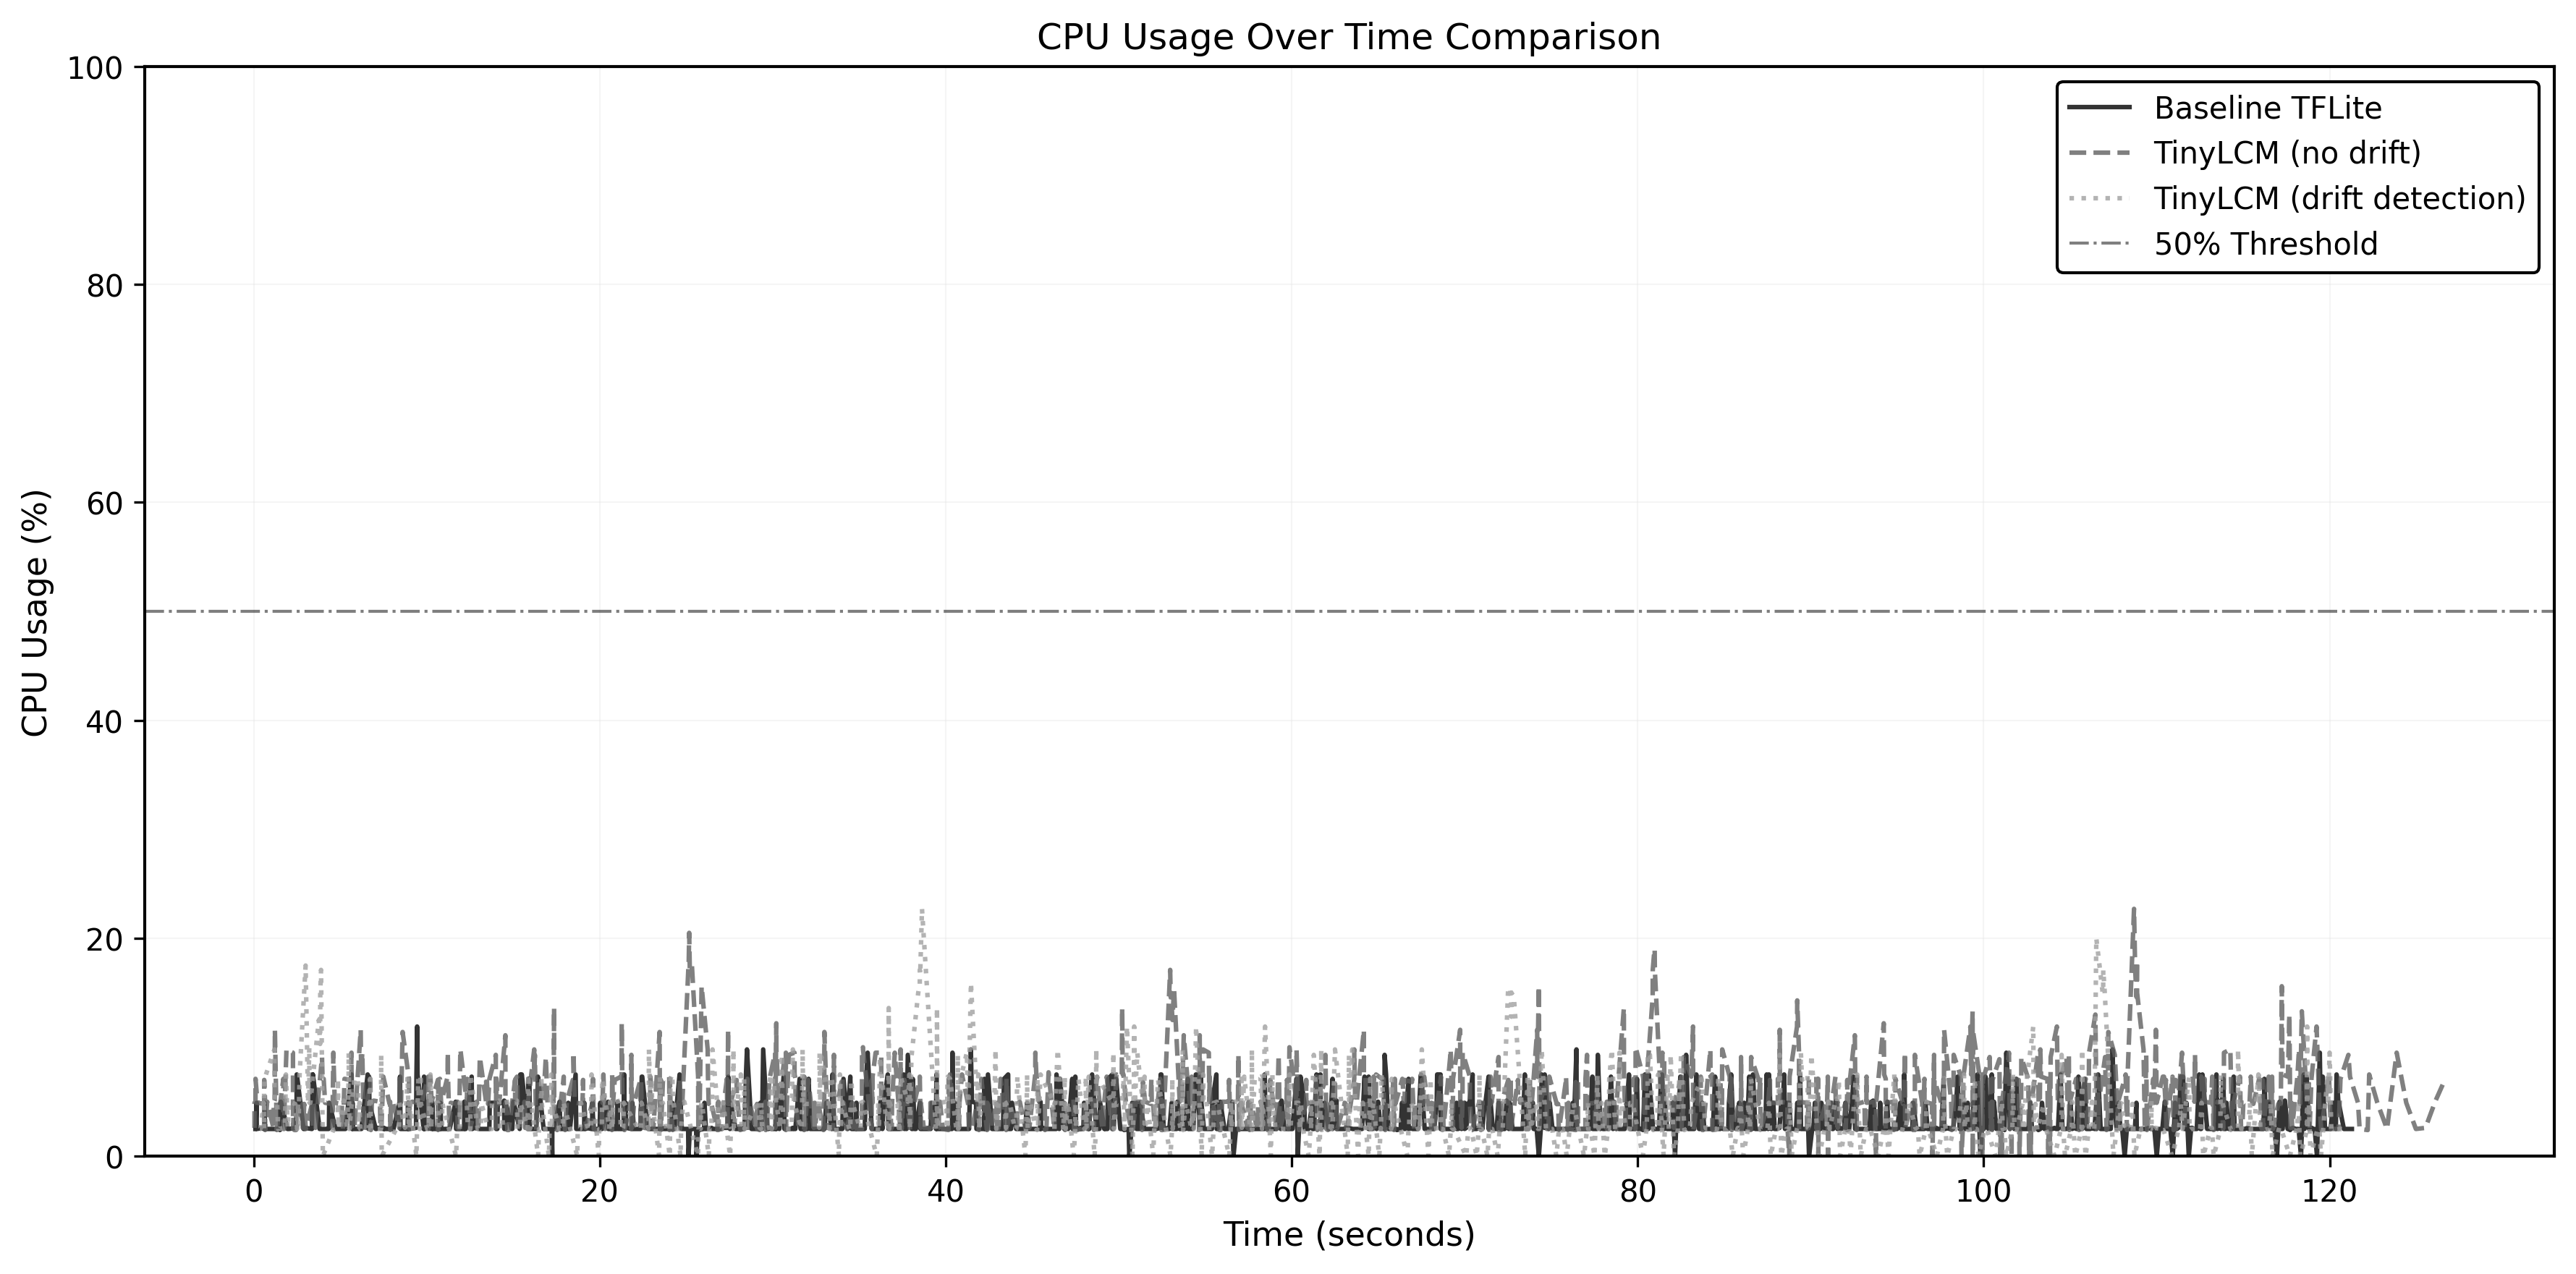
\includegraphics[width=0.98\textwidth]{figs/evaluation/cpu_timeseries.png}
    \caption[CPU Comparison]{Time series diagram comparing the CPU utilization of the different approaches.}
    \label{fig:cpu-comparison}
\end{figure}




%%%%%%%%%%%%%%%%%%%%%%%%%%%%%%%%%%%%%%%%%%%%%
%% Bibliography

%\nocite{*}
%\bibliographystyle{geralpha}
\bibliographystyle{plain}
\bibliography{thesis}
%\bibliography{bibtex}
\vfill
%\pagebreak

\end{document}
